\documentclass[%
 reprint,
%superscriptaddress,
%groupedaddress,
%unsortedaddress,
%runinaddress,
%frontmatterverbose, 
%preprint,
%showpacs,preprintnumbers,
%nofootinbib,
%nobibnotes,
%bibnotes,
 amsmath,amssymb,
 aps, prl
]{revtex4-1}

\usepackage{graphicx}% Include figure files
\usepackage{dcolumn}% Align table columns on decimal point
\usepackage{bm}% bold math
\usepackage{hyperref}% add hypertext capabilities
%\usepackage[mathlines]{lineno}% Enable numbering of text and display math
%\linenumbers\relax % Commence numbering lines

% --- LHCb specfic ----
\usepackage{ifthen} % for conditional statements
\newboolean{pdflatex}
\setboolean{pdflatex}{true} % False for eps figures 

\newboolean{articletitles}
\setboolean{articletitles}{true} % False removes titles in references

\newboolean{uprightparticles}
\setboolean{uprightparticles}{false} %True for upright particle symbols

%\newboolean{inbibliography}
%\setboolean{inbibliography}{false} %True once you enter the bibliography

\newboolean{wordcount}
\setboolean{wordcount}{true} % False for normal usage; true for wordcount.sh

\ifthenelse{\boolean{wordcount}}%
{\usepackage{bibentry} % For nobibliography command
 \usepackage{mciteplus} % combine multiple citations
 \usepackage{comment} % comment lines
 % Uncomment the lines below to exclude equations from the word count
 %\excludecomment{align*} % Remove align*
 %\excludecomment{align} % Remove align
 %\let\endalign\relax % Remove align
 %\excludecomment{equation*} % Remove equation* (does not work)
 %\excludecomment{equation} % Remove equation
 %\let\endequation\relax % Remove equation
 %\excludecomment{eqnarray*} % Remove eqnarray*
 %\excludecomment{eqnarray} % Remove eqnarray
 %\let\endeqnarray\relax % Remove eqnarray
 \excludecomment{acknowledgments} % Remove acknowledgments
 \let\endacknowledgments\relax % Remove acknowledgments
 \def\maketitle{} % Remove title and abstract
}{
}

\graphicspath{{./figs/}}
\DeclareGraphicsExtensions{.pdf,.PDF,png,.PNG}
\usepackage{xspace} 
\makeatletter
\gdef\@ptsize{0} % fix miniscule font definition from lhcb-symbols
\makeatother
\let\put\relax % avoid \put commands in a PRL paper 
% Remove the Acknowledgement heading for PRL
\makeatletter
\usepackage{suffix}
\let\latex@section\section
\WithSuffix\def\section*{\secdef\my@section{\latex@section*}}
\def\my@section[#1]#2{}
\makeatother

%%%%%%%%%%%%%%%%%%%%%%%%%%%%%%%%%%%%%%%%%%%%%%%%%%%%%%%%%%%%%%%%%%%%%%%%
%%%                                                                    %
%%% !!!!!!!!!!!!!!!!!!! DO NOT EDIT THIS FILE !!!!!!!!!!!!!!!!!!!!!!!! %
%%%                                                                    %
%%% THE EB MAY OVERWRITE IT TO REFLECT LATEST CHANGES IN THE TEMPLATE  %
%%%                                                                    %
%%% You may define your own macros and packages in main.tex or add     %
%%% additional local files                                             %
%%%%%%%%%%%%%%%%%%%%%%%%%%%%%%%%%%%%%%%%%%%%%%%%%%%%%%%%%%%%%%%%%%%%%%%%
%%% ======================================================================
%%% Purpose: Standard LHCb aliases
%%% Author: Originally Ulrik Egede, adapted by Tomasz Skwarnicki for templates,
%%% rewritten by Chris Parkes
%%% Maintainer : Ulrik Egede (2010 - 2012)
%%% Maintainer : Rolf Oldeman (2012 - 2014)
%%% Maintainer : Patrick Koppenburg (2018--2020)
%%% =======================================================================
%%% To use this file outside the normal LHCb document environment, the
%%% following should be added in a preamble (before \begin{document}
%%%
%%%\usepackage{ifthen} 
%%%\newboolean{uprightparticles}
%%%\setboolean{uprightparticles}{false} %Set true for upright particle symbols
\usepackage{xspace} 
\usepackage{upgreek}


%%%%%%%%%%%%%%%%%%%%%%%%%%%%%%%%%%%%%%%%%%%%%%%%%%%%%%%%%%%%
%%%
%%% The following is to ensure that the template automatically can process
%%% this file.
%%%
%%% Add comments with at least three %%% preceding.
%%% Add new sections with one % preceding
%%% Add new subsections with two %% preceding
%%%
%%% For upper greek letters, Xires and Xiresbar will be the particles without the charge
%%% States with charge are called Xiz and Xim  
%%%
%%%%%%%%%%%%%%%%%%%%%%%%%%%%%%%%%%%%%%%%%%%%%%%%%%%%%%%%%%%%

%%%%%%%%%%%%%
% Experiments
%%%%%%%%%%%%%
\def\lhcb   {\mbox{LHCb}\xspace}
\def\atlas  {\mbox{ATLAS}\xspace}
\def\cms    {\mbox{CMS}\xspace}
\def\alice  {\mbox{ALICE}\xspace}
\def\babar  {\mbox{BaBar}\xspace}
\def\belle  {\mbox{Belle}\xspace}
\def\belletwo {\mbox{Belle~II}\xspace}
\def\besiii {\mbox{BESIII}\xspace}
\def\cleo   {\mbox{CLEO}\xspace}
\def\cdf    {\mbox{CDF}\xspace}
\def\dzero  {\mbox{D0}\xspace}
\def\aleph  {\mbox{ALEPH}\xspace}
\def\delphi {\mbox{DELPHI}\xspace}
\def\opal   {\mbox{OPAL}\xspace}
\def\lthree {\mbox{L3}\xspace}
\def\sld    {\mbox{SLD}\xspace}
%%%\def\argus  {\mbox{ARGUS}\xspace}
%%%\def\uaone  {\mbox{UA1}\xspace}
%%%\def\uatwo  {\mbox{UA2}\xspace}
%%%\def\ux85 {\mbox{UX85}\xspace}
\def\cern {\mbox{CERN}\xspace}
\def\lhc    {\mbox{LHC}\xspace}
\def\lep    {\mbox{LEP}\xspace}
\def\tevatron {Tevatron\xspace}
\def\bfactories {\mbox{\B Factories}\xspace}
\def\bfactory   {\mbox{\B Factory}\xspace}
\def\upgradeone {\mbox{Upgrade~I}\xspace}
\def\upgradetwo {\mbox{Upgrade~II}\xspace}

%% LHCb sub-detectors and sub-systems

%%%\def\pu     {PU\xspace}
\def\velo   {VELO\xspace}
\def\rich   {RICH\xspace}
\def\richone {RICH1\xspace}
\def\richtwo {RICH2\xspace}
\def\ttracker {TT\xspace}
\def\intr   {IT\xspace}
\def\st     {ST\xspace}
\def\ot     {OT\xspace}
\def\herschel {\mbox{\textsc{HeRSCheL}}\xspace}
%%%\def\Tone   {T1\xspace}
%%%\def\Ttwo   {T2\xspace}
%%%\def\Tthree {T3\xspace}
%%%\def\Mone   {M1\xspace}
%%%\def\Mtwo   {M2\xspace}
%%%\def\Mthree {M3\xspace}
%%%\def\Mfour  {M4\xspace}
%%%\def\Mfive  {M5\xspace}
\def\spd    {SPD\xspace}
\def\presh  {PS\xspace}
\def\ecal   {ECAL\xspace}
\def\hcal   {HCAL\xspace}
%%%\def\bcm    {BCM\xspace}
\def\MagUp {\mbox{\em Mag\kern -0.05em Up}\xspace}
\def\MagDown {\mbox{\em MagDown}\xspace}

\def\ode    {ODE\xspace}
\def\daq    {DAQ\xspace}
\def\tfc    {TFC\xspace}
\def\ecs    {ECS\xspace}
\def\lone   {L0\xspace}
\def\hlt    {HLT\xspace}
\def\hltone {HLT1\xspace}
\def\hlttwo {HLT2\xspace}

%%% Upright (not slanted) Particles

\ifthenelse{\boolean{uprightparticles}}%
{\def\Palpha      {\ensuremath{\upalpha}\xspace}
 \def\Pbeta       {\ensuremath{\upbeta}\xspace}
 \def\Pgamma      {\ensuremath{\upgamma}\xspace}                 
 \def\Pdelta      {\ensuremath{\updelta}\xspace}                 
 \def\Pepsilon    {\ensuremath{\upepsilon}\xspace}                 
 \def\Pvarepsilon {\ensuremath{\upvarepsilon}\xspace}                 
 \def\Pzeta       {\ensuremath{\upzeta}\xspace}                 
 \def\Peta        {\ensuremath{\upeta}\xspace}
 \def\Ptheta      {\ensuremath{\uptheta}\xspace}                 
 \def\Pvartheta   {\ensuremath{\upvartheta}\xspace}                 
 \def\Piota       {\ensuremath{\upiota}\xspace}                 
 \def\Pkappa      {\ensuremath{\upkappa}\xspace}                 
 \def\Plambda     {\ensuremath{\uplambda}\xspace}                 
 \def\Pmu         {\ensuremath{\upmu}\xspace}                 
 \def\Pnu         {\ensuremath{\upnu}\xspace}                 
 \def\Pxi         {\ensuremath{\upxi}\xspace}                 
 \def\Ppi         {\ensuremath{\uppi}\xspace}                 
 \def\Pvarpi      {\ensuremath{\upvarpi}\xspace}                 
 \def\Prho        {\ensuremath{\uprho}\xspace}                 
 \def\Pvarrho     {\ensuremath{\upvarrho}\xspace}                 
 \def\Ptau        {\ensuremath{\uptau}\xspace}                 
 \def\Pupsilon    {\ensuremath{\upupsilon}\xspace}                 
 \def\Pphi        {\ensuremath{\upphi}\xspace}                 
 \def\Pvarphi     {\ensuremath{\upvarphi}\xspace}                 
 \def\Pchi        {\ensuremath{\upchi}\xspace}                 
 \def\Ppsi        {\ensuremath{\uppsi}\xspace}                 
 \def\Pomega      {\ensuremath{\upomega}\xspace}                 

 \def\PDelta      {\ensuremath{\Delta}\xspace}                 
 \def\PXi         {\ensuremath{\Xi}\xspace}                 
 \def\PLambda     {\ensuremath{\Lambda}\xspace}                 
 \def\PSigma      {\ensuremath{\Sigma}\xspace}                 
 \def\POmega      {\ensuremath{\Omega}\xspace}                 
 \def\PUpsilon    {\ensuremath{\Upsilon}\xspace}
 \let\oldPi\Pi
 \def\PPi         {\ensuremath{\oldPi}\xspace}                 
               

 \def\PA      {\ensuremath{\mathrm{A}}\xspace}                 
 \def\PB      {\ensuremath{\mathrm{B}}\xspace}                 
 \def\PC      {\ensuremath{\mathrm{C}}\xspace}                 
 \def\PD      {\ensuremath{\mathrm{D}}\xspace}                 
 \def\PE      {\ensuremath{\mathrm{E}}\xspace}                 
 \def\PF      {\ensuremath{\mathrm{F}}\xspace}                 
 \def\PG      {\ensuremath{\mathrm{G}}\xspace}                 
 \def\PH      {\ensuremath{\mathrm{H}}\xspace}                 
 \def\PI      {\ensuremath{\mathrm{I}}\xspace}                 
 \def\PJ      {\ensuremath{\mathrm{J}}\xspace}                 
 \def\PK      {\ensuremath{\mathrm{K}}\xspace}                 
 \def\PL      {\ensuremath{\mathrm{L}}\xspace}                 
 \def\PM      {\ensuremath{\mathrm{M}}\xspace}                 
 \def\PN      {\ensuremath{\mathrm{N}}\xspace}                 
 \def\PO      {\ensuremath{\mathrm{O}}\xspace}                 
 \def\PP      {\ensuremath{\mathrm{P}}\xspace}                 
 \def\PQ      {\ensuremath{\mathrm{Q}}\xspace}                 
 \def\PR      {\ensuremath{\mathrm{R}}\xspace}                 
 \def\PS      {\ensuremath{\mathrm{S}}\xspace}                 
 \def\PT      {\ensuremath{\mathrm{T}}\xspace}                 
 \def\PU      {\ensuremath{\mathrm{U}}\xspace}                 
 \def\PV      {\ensuremath{\mathrm{V}}\xspace}                 
 \def\PW      {\ensuremath{\mathrm{W}}\xspace}                 
 \def\PX      {\ensuremath{\mathrm{X}}\xspace}                 
 \def\PY      {\ensuremath{\mathrm{Y}}\xspace}                 
 \def\PZ      {\ensuremath{\mathrm{Z}}\xspace}                 
 \def\Pa      {\ensuremath{\mathrm{a}}\xspace}                 
 \def\Pb      {\ensuremath{\mathrm{b}}\xspace}                 
 \def\Pc      {\ensuremath{\mathrm{c}}\xspace}                 
 \def\Pd      {\ensuremath{\mathrm{d}}\xspace}                 
 \def\Pe      {\ensuremath{\mathrm{e}}\xspace}                 
 \def\Pf      {\ensuremath{\mathrm{f}}\xspace}                 
 \def\Pg      {\ensuremath{\mathrm{g}}\xspace}                 
 \def\Ph      {\ensuremath{\mathrm{h}}\xspace}                 
 \def\Pi      {\ensuremath{\mathrm{i}}\xspace}                 
 \def\Pj      {\ensuremath{\mathrm{j}}\xspace}                 
 \def\Pk      {\ensuremath{\mathrm{k}}\xspace}                 
 \def\Pl      {\ensuremath{\mathrm{l}}\xspace}                 
 \def\Pm      {\ensuremath{\mathrm{m}}\xspace}                 
 \def\Pn      {\ensuremath{\mathrm{n}}\xspace}                 
 \def\Po      {\ensuremath{\mathrm{o}}\xspace}                 
 \def\Pp      {\ensuremath{\mathrm{p}}\xspace}                 
 \def\Pq      {\ensuremath{\mathrm{q}}\xspace}                 
 \def\Pr      {\ensuremath{\mathrm{r}}\xspace}                 
 \def\Ps      {\ensuremath{\mathrm{s}}\xspace}                 
 \def\Pt      {\ensuremath{\mathrm{t}}\xspace}                 
 \def\Pu      {\ensuremath{\mathrm{u}}\xspace}                 
 \def\Pv      {\ensuremath{\mathrm{v}}\xspace}                 
 \def\Pw      {\ensuremath{\mathrm{w}}\xspace}                 
 \def\Px      {\ensuremath{\mathrm{x}}\xspace}                 
 \def\Py      {\ensuremath{\mathrm{y}}\xspace}                 
 \def\Pz      {\ensuremath{\mathrm{z}}\xspace}                 
 \def\thebaroffset{0.0em}
}
{\def\Palpha      {\ensuremath{\alpha}\xspace}
 \def\Pbeta       {\ensuremath{\beta}\xspace}
 \def\Pgamma      {\ensuremath{\gamma}\xspace}                 
 \def\Pdelta      {\ensuremath{\delta}\xspace}                 
 \def\Pepsilon    {\ensuremath{\epsilon}\xspace}                 
 \def\Pvarepsilon {\ensuremath{\varepsilon}\xspace}                 
 \def\Pzeta       {\ensuremath{\zeta}\xspace}                 
 \def\Peta        {\ensuremath{\eta}\xspace}                 
 \def\Ptheta      {\ensuremath{\theta}\xspace}                 
 \def\Pvartheta   {\ensuremath{\vartheta}\xspace}                 
 \def\Piota       {\ensuremath{\iota}\xspace}                 
 \def\Pkappa      {\ensuremath{\kappa}\xspace}                 
 \def\Plambda     {\ensuremath{\lambda}\xspace}                 
 \def\Pmu         {\ensuremath{\mu}\xspace}                 
 \def\Pnu         {\ensuremath{\nu}\xspace}                 
 \def\Pxi         {\ensuremath{\xi}\xspace}                 
 \def\Ppi         {\ensuremath{\pi}\xspace}                 
 \def\Pvarpi      {\ensuremath{\varpi}\xspace}                 
 \def\Prho        {\ensuremath{\rho}\xspace}                 
 \def\Pvarrho     {\ensuremath{\varrho}\xspace}                 
 \def\Ptau        {\ensuremath{\tau}\xspace}                 
 \def\Pupsilon    {\ensuremath{\upsilon}\xspace}                 
 \def\Pphi        {\ensuremath{\phi}\xspace}                 
 \def\Pvarphi     {\ensuremath{\varphi}\xspace}                 
 \def\Pchi        {\ensuremath{\chi}\xspace}                 
 \def\Ppsi        {\ensuremath{\psi}\xspace}                 
 \def\Pomega      {\ensuremath{\omega}\xspace}                 
 \mathchardef\PDelta="7101
 \mathchardef\PXi="7104
 \mathchardef\PLambda="7103
 \mathchardef\PSigma="7106
 \mathchardef\POmega="710A
 \mathchardef\PUpsilon="7107
 \mathchardef\PPi="7105
 \def\PA      {\ensuremath{A}\xspace}                 
 \def\PB      {\ensuremath{B}\xspace}                 
 \def\PC      {\ensuremath{C}\xspace}                 
 \def\PD      {\ensuremath{D}\xspace}                 
 \def\PE      {\ensuremath{E}\xspace}                 
 \def\PF      {\ensuremath{F}\xspace}                 
 \def\PG      {\ensuremath{G}\xspace}                 
 \def\PH      {\ensuremath{H}\xspace}                 
 \def\PI      {\ensuremath{I}\xspace}                 
 \def\PJ      {\ensuremath{J}\xspace}                 
 \def\PK      {\ensuremath{K}\xspace}                 
 \def\PL      {\ensuremath{L}\xspace}                 
 \def\PM      {\ensuremath{M}\xspace}                 
 \def\PN      {\ensuremath{N}\xspace}                 
 \def\PO      {\ensuremath{O}\xspace}                 
 \def\PP      {\ensuremath{P}\xspace}                 
 \def\PQ      {\ensuremath{Q}\xspace}                 
 \def\PR      {\ensuremath{R}\xspace}                 
 \def\PS      {\ensuremath{S}\xspace}                 
 \def\PT      {\ensuremath{T}\xspace}                 
 \def\PU      {\ensuremath{U}\xspace}                 
 \def\PV      {\ensuremath{V}\xspace}                 
 \def\PW      {\ensuremath{W}\xspace}                 
 \def\PX      {\ensuremath{X}\xspace}                 
 \def\PY      {\ensuremath{Y}\xspace}                 
 \def\PZ      {\ensuremath{Z}\xspace}                 
 \def\Pa      {\ensuremath{a}\xspace}                 
 \def\Pb      {\ensuremath{b}\xspace}                 
 \def\Pc      {\ensuremath{c}\xspace}                 
 \def\Pd      {\ensuremath{d}\xspace}                 
 \def\Pe      {\ensuremath{e}\xspace}                 
 \def\Pf      {\ensuremath{f}\xspace}                 
 \def\Pg      {\ensuremath{g}\xspace}                 
 \def\Ph      {\ensuremath{h}\xspace}                 
 \def\Pi      {\ensuremath{i}\xspace}                 
 \def\Pj      {\ensuremath{j}\xspace}                 
 \def\Pk      {\ensuremath{k}\xspace}                 
 \def\Pl      {\ensuremath{l}\xspace}                 
 \def\Pm      {\ensuremath{m}\xspace}                 
 \def\Pn      {\ensuremath{n}\xspace}                 
 \def\Po      {\ensuremath{o}\xspace}                 
 \def\Pp      {\ensuremath{p}\xspace}                 
 \def\Pq      {\ensuremath{q}\xspace}                 
 \def\Pr      {\ensuremath{r}\xspace}                 
 \def\Ps      {\ensuremath{s}\xspace}                 
 \def\Pt      {\ensuremath{t}\xspace}                 
 \def\Pu      {\ensuremath{u}\xspace}                 
 \def\Pv      {\ensuremath{v}\xspace}                 
 \def\Pw      {\ensuremath{w}\xspace}                 
 \def\Px      {\ensuremath{x}\xspace}                 
 \def\Py      {\ensuremath{y}\xspace}                 
 \def\Pz      {\ensuremath{z}\xspace}
 \def\thebaroffset{0.18em}
}
\newcommand{\offsetoverline}[2][\thebaroffset]{\kern #1\overline{\kern -#1 #2}}%

%%%%%%%%%%%%%%%%%%%%%%%%%%%%%%%%%%%%%%%%%%%%%%%
% Particles
\makeatletter
\ifcase \@ptsize \relax% 10pt
  \newcommand{\miniscule}{\@setfontsize\miniscule{4}{5}}% \tiny: 5/6
\or% 11pt
  \newcommand{\miniscule}{\@setfontsize\miniscule{5}{6}}% \tiny: 6/7
\or% 12pt
  \newcommand{\miniscule}{\@setfontsize\miniscule{5}{6}}% \tiny: 6/7
\fi
\makeatother


\DeclareRobustCommand{\optbar}[1]{\shortstack{{\miniscule (\rule[.5ex]{1.25em}{.18mm})}
  \\ [-.7ex] $#1$}}


%% Leptons

\let\emi\en
\def\electron   {{\ensuremath{\Pe}}\xspace}
\def\en         {{\ensuremath{\Pe^-}}\xspace}   % electron negative (\em is taken)
\def\ep         {{\ensuremath{\Pe^+}}\xspace}
\def\epm        {{\ensuremath{\Pe^\pm}}\xspace} 
\def\emp        {{\ensuremath{\Pe^\mp}}\xspace} 
\def\epem       {{\ensuremath{\Pe^+\Pe^-}}\xspace}
%%%\def\ee         {\ensuremath{\Pe^-\Pe^-}\xspace}

\def\muon       {{\ensuremath{\Pmu}}\xspace}
\def\mup        {{\ensuremath{\Pmu^+}}\xspace}
\def\mun        {{\ensuremath{\Pmu^-}}\xspace} % muon negative (\mum is taken)
\def\mupm       {{\ensuremath{\Pmu^\pm}}\xspace} 
\def\mump       {{\ensuremath{\Pmu^\mp}}\xspace} 
\def\mumu       {{\ensuremath{\Pmu^+\Pmu^-}}\xspace}

\def\tauon      {{\ensuremath{\Ptau}}\xspace}
\def\taup       {{\ensuremath{\Ptau^+}}\xspace}
\def\taum       {{\ensuremath{\Ptau^-}}\xspace}
\def\taupm      {{\ensuremath{\Ptau^\pm}}\xspace}
\def\taump      {{\ensuremath{\Ptau^\mp}}\xspace}
\def\tautau     {{\ensuremath{\Ptau^+\Ptau^-}}\xspace}

\def\lepton     {{\ensuremath{\ell}}\xspace}
\def\ellm       {{\ensuremath{\ell^-}}\xspace}
\def\ellp       {{\ensuremath{\ell^+}}\xspace}
\def\ellpm      {{\ensuremath{\ell^\pm}}\xspace}
\def\ellmp      {{\ensuremath{\ell^\mp}}\xspace}
\def\ellell     {\ensuremath{\ell^+ \ell^-}\xspace}

\def\neu        {{\ensuremath{\Pnu}}\xspace}
\def\neub       {{\ensuremath{\overline{\Pnu}}}\xspace}
%%%\def\nuenueb    {\ensuremath{\neu\neub}\xspace}
\def\neue       {{\ensuremath{\neu_e}}\xspace}
\def\neueb      {{\ensuremath{\neub_e}}\xspace}
%%%\def\neueneueb  {\ensuremath{\neue\neueb}\xspace}
\def\neum       {{\ensuremath{\neu_\mu}}\xspace}
\def\neumb      {{\ensuremath{\neub_\mu}}\xspace}
%%%\def\neumneumb  {\ensuremath{\neum\neumb}\xspace}
\def\neut       {{\ensuremath{\neu_\tau}}\xspace}
\def\neutb      {{\ensuremath{\neub_\tau}}\xspace}
%%%\def\neutneutb  {\ensuremath{\neut\neutb}\xspace}
\def\neul       {{\ensuremath{\neu_\ell}}\xspace}
\def\neulb      {{\ensuremath{\neub_\ell}}\xspace}
%%%\def\neulneulb  {\ensuremath{\neul\neulb}\xspace}

%% Gauge bosons and scalars

\def\g      {{\ensuremath{\Pgamma}}\xspace}
\def\H      {{\ensuremath{\PH^0}}\xspace}
\def\Hp     {{\ensuremath{\PH^+}}\xspace}
\def\Hm     {{\ensuremath{\PH^-}}\xspace}
\def\Hpm    {{\ensuremath{\PH^\pm}}\xspace}
\def\W      {{\ensuremath{\PW}}\xspace}
\def\Wp     {{\ensuremath{\PW^+}}\xspace}
\def\Wm     {{\ensuremath{\PW^-}}\xspace}
\def\Wpm    {{\ensuremath{\PW^\pm}}\xspace}
\def\Z      {{\ensuremath{\PZ}}\xspace}

%% Quarks

\def\quark     {{\ensuremath{\Pq}}\xspace}
\def\quarkbar  {{\ensuremath{\overline \quark}}\xspace}
\def\qqbar     {{\ensuremath{\quark\quarkbar}}\xspace}
\def\uquark    {{\ensuremath{\Pu}}\xspace}
\def\uquarkbar {{\ensuremath{\overline \uquark}}\xspace}
\def\uubar     {{\ensuremath{\uquark\uquarkbar}}\xspace}
\def\dquark    {{\ensuremath{\Pd}}\xspace}
\def\dquarkbar {{\ensuremath{\overline \dquark}}\xspace}
\def\ddbar     {{\ensuremath{\dquark\dquarkbar}}\xspace}
\def\squark    {{\ensuremath{\Ps}}\xspace}
\def\squarkbar {{\ensuremath{\overline \squark}}\xspace}
\def\ssbar     {{\ensuremath{\squark\squarkbar}}\xspace}
\def\cquark    {{\ensuremath{\Pc}}\xspace}
\def\cquarkbar {{\ensuremath{\overline \cquark}}\xspace}
\def\ccbar     {{\ensuremath{\cquark\cquarkbar}}\xspace}
\def\bquark    {{\ensuremath{\Pb}}\xspace}
\def\bquarkbar {{\ensuremath{\overline \bquark}}\xspace}
\def\bbbar     {{\ensuremath{\bquark\bquarkbar}}\xspace}
\def\tquark    {{\ensuremath{\Pt}}\xspace}
\def\tquarkbar {{\ensuremath{\overline \tquark}}\xspace}
\def\ttbar     {{\ensuremath{\tquark\tquarkbar}}\xspace}

%% Light mesons

\def\hadron {{\ensuremath{\Ph}}\xspace}
\def\pion   {{\ensuremath{\Ppi}}\xspace}
\def\piz    {{\ensuremath{\pion^0}}\xspace}
\def\pip    {{\ensuremath{\pion^+}}\xspace}
\def\pim    {{\ensuremath{\pion^-}}\xspace}
\def\pipm   {{\ensuremath{\pion^\pm}}\xspace}
\def\pimp   {{\ensuremath{\pion^\mp}}\xspace}

\def\rhomeson {{\ensuremath{\Prho}}\xspace}
\def\rhoz     {{\ensuremath{\rhomeson^0}}\xspace}
\def\rhop     {{\ensuremath{\rhomeson^+}}\xspace}
\def\rhom     {{\ensuremath{\rhomeson^-}}\xspace}
\def\rhopm    {{\ensuremath{\rhomeson^\pm}}\xspace}
\def\rhomp    {{\ensuremath{\rhomeson^\mp}}\xspace}

\def\kaon    {{\ensuremath{\PK}}\xspace}
%%% do NOT use ensuremath here, and keep indent
\def\Kbar    {{\ensuremath{\offsetoverline{\PK}}}\xspace}
\def\Kb      {{\ensuremath{\Kbar}}\xspace}
\def\KorKbar {\kern \thebaroffset\optbar{\kern -\thebaroffset \PK}{}\xspace}
\def\Kz      {{\ensuremath{\kaon^0}}\xspace}
\def\Kzb     {{\ensuremath{\Kbar{}^0}}\xspace}
\def\Kp      {{\ensuremath{\kaon^+}}\xspace}
\def\Km      {{\ensuremath{\kaon^-}}\xspace}
\def\Kpm     {{\ensuremath{\kaon^\pm}}\xspace}
\def\Kmp     {{\ensuremath{\kaon^\mp}}\xspace}
\def\KS      {{\ensuremath{\kaon^0_{\mathrm{S}}}}\xspace}
\def\Vzero   {{\ensuremath{V^0}}\xspace}
\def\KL      {{\ensuremath{\kaon^0_{\mathrm{L}}}}\xspace}
\def\Kstarz  {{\ensuremath{\kaon^{*0}}}\xspace}
\def\Kstarzb {{\ensuremath{\Kbar{}^{*0}}}\xspace}
\def\Kstar   {{\ensuremath{\kaon^*}}\xspace}
\def\Kstarb  {{\ensuremath{\Kbar{}^*}}\xspace}
\def\Kstarp  {{\ensuremath{\kaon^{*+}}}\xspace}
\def\Kstarm  {{\ensuremath{\kaon^{*-}}}\xspace}
\def\Kstarpm {{\ensuremath{\kaon^{*\pm}}}\xspace}
\def\Kstarmp {{\ensuremath{\kaon^{*\mp}}}\xspace}
\def\KorKbarz {\ensuremath{\KorKbar^0}\xspace}

\newcommand{\etaz}{\ensuremath{\Peta}\xspace}
\newcommand{\etapr}{\ensuremath{\Peta^{\prime}}\xspace}
\newcommand{\phiz}{\ensuremath{\Pphi}\xspace}
\newcommand{\omegaz}{\ensuremath{\Pomega}\xspace}

%% Charmed mesons

%%% do NOT use ensuremath here (and keep indent)
\def\Dbar    {{\ensuremath{\offsetoverline{\PD}}}\xspace}
\def\D       {{\ensuremath{\PD}}\xspace}
\def\Db      {{\ensuremath{\Dbar}}\xspace}
\def\DorDbar {\kern \thebaroffset\optbar{\kern -\thebaroffset \PD}\xspace}
\def\Dz      {{\ensuremath{\D^0}}\xspace}
\def\Dzb     {{\ensuremath{\Dbar{}^0}}\xspace}
\def\Dp      {{\ensuremath{\D^+}}\xspace}
\def\Dm      {{\ensuremath{\D^-}}\xspace}
\def\Dpm     {{\ensuremath{\D^\pm}}\xspace}
\def\Dmp     {{\ensuremath{\D^\mp}}\xspace}
\def\DpDm    {\ensuremath{\Dp {\kern -0.16em \Dm}}\xspace}
\def\Dstar   {{\ensuremath{\D^*}}\xspace}
\def\Dstarb  {{\ensuremath{\Dbar{}^*}}\xspace}
\def\Dstarz  {{\ensuremath{\D^{*0}}}\xspace}
\def\Dstarzb {{\ensuremath{\Dbar{}^{*0}}}\xspace}
\def\theDstarz{{\ensuremath{\D^{*}(2007)^{0}}}\xspace}
\def\theDstarzb{{\ensuremath{\Dbar^{*}(2007)^{0}}}\xspace}
\def\Dstarp  {{\ensuremath{\D^{*+}}}\xspace}
\def\Dstarm  {{\ensuremath{\D^{*-}}}\xspace}
\def\Dstarpm {{\ensuremath{\D^{*\pm}}}\xspace}
\def\Dstarmp {{\ensuremath{\D^{*\mp}}}\xspace}
\def\theDstarp{{\ensuremath{\D^{*}(2010)^{+}}}\xspace}
\def\theDstarm{{\ensuremath{\D^{*}(2010)^{-}}}\xspace}
\def\theDstarpm{{\ensuremath{\D^{*}(2010)^{\pm}}}\xspace}
\def\theDstarmp{{\ensuremath{\D^{*}(2010)^{\mp}}}\xspace}
\def\Ds      {{\ensuremath{\D^+_\squark}}\xspace}
\def\Dsp     {{\ensuremath{\D^+_\squark}}\xspace}
\def\Dsm     {{\ensuremath{\D^-_\squark}}\xspace}
\def\Dspm    {{\ensuremath{\D^{\pm}_\squark}}\xspace}
\def\Dsmp    {{\ensuremath{\D^{\mp}_\squark}}\xspace}
\def\Dss     {{\ensuremath{\D^{*+}_\squark}}\xspace}
\def\Dssp    {{\ensuremath{\D^{*+}_\squark}}\xspace}
\def\Dssm    {{\ensuremath{\D^{*-}_\squark}}\xspace}
\def\Dsspm   {{\ensuremath{\D^{*\pm}_\squark}}\xspace}
\def\Dssmp   {{\ensuremath{\D^{*\mp}_\squark}}\xspace}
\def\DporDsp {{\ensuremath{\D_{(\squark)}^+}}\xspace}
\def\DmorDsm {{\ensuremath{\D{}_{(\squark)}^-}}\xspace}
\def\DpmorDspm {{\ensuremath{\D{}_{(\squark)}^\pm}}\xspace}

%% Beauty mesons
\def\B       {{\ensuremath{\PB}}\xspace}
\def\Bbar    {{\ensuremath{\offsetoverline{\PB}}}\xspace}
\def\Bb      {{\ensuremath{\Bbar}}\xspace}
\def\BorBbar {\kern \thebaroffset\optbar{\kern -\thebaroffset \PB}\xspace}
\def\Bz      {{\ensuremath{\B^0}}\xspace}
\def\Bzb     {{\ensuremath{\Bbar{}^0}}\xspace}
\def\Bd      {{\ensuremath{\B^0}}\xspace}
\def\Bdb     {{\ensuremath{\Bbar{}^0}}\xspace}
\def\BdorBdbar {\kern \thebaroffset\optbar{\kern -\thebaroffset \Bd}\xspace}
\def\Bu      {{\ensuremath{\B^+}}\xspace}
\def\Bub     {{\ensuremath{\B^-}}\xspace}
\def\Bp      {{\ensuremath{\Bu}}\xspace}
\def\Bm      {{\ensuremath{\Bub}}\xspace}
\def\Bpm     {{\ensuremath{\B^\pm}}\xspace}
\def\Bmp     {{\ensuremath{\B^\mp}}\xspace}
\def\Bs      {{\ensuremath{\B^0_\squark}}\xspace}
\def\Bsb     {{\ensuremath{\Bbar{}^0_\squark}}\xspace}
\def\BsorBsbar {\kern \thebaroffset\optbar{\kern -\thebaroffset \Bs}\xspace}
\def\Bc      {{\ensuremath{\B_\cquark^+}}\xspace}
\def\Bcp     {{\ensuremath{\B_\cquark^+}}\xspace}
\def\Bcm     {{\ensuremath{\B_\cquark^-}}\xspace}
\def\Bcpm    {{\ensuremath{\B_\cquark^\pm}}\xspace}
\def\Bds     {{\ensuremath{\B_{(\squark)}^0}}\xspace}
\def\Bdsb    {{\ensuremath{\Bbar{}_{(\squark)}^0}}\xspace}
\def\BdorBs  {\Bds}
\def\BdorBsbar  {\Bdsb}

%% Onia

\def\jpsi     {{\ensuremath{{\PJ\mskip -3mu/\mskip -2mu\Ppsi}}}\xspace}
\def\psitwos  {{\ensuremath{\Ppsi{(2S)}}}\xspace}
\def\psiprpr  {{\ensuremath{\Ppsi(3770)}}\xspace}
\def\etac     {{\ensuremath{\Peta_\cquark}}\xspace}
\def\psires  {{\ensuremath{\Ppsi}}\xspace}
\def\chic     {{\ensuremath{\Pchi_\cquark}}\xspace}
\def\chiczero {{\ensuremath{\Pchi_{\cquark 0}}}\xspace}
\def\chicone  {{\ensuremath{\Pchi_{\cquark 1}}}\xspace}
\def\chictwo  {{\ensuremath{\Pchi_{\cquark 2}}}\xspace}
\def\chicJ    {{\ensuremath{\Pchi_{\cquark J}}}\xspace}
\def\Upsilonres  {{\ensuremath{\PUpsilon}}\xspace}
\def\Y#1S{\ensuremath{\PUpsilon{(#1S)}}\xspace}
\def\OneS  {{\Y1S}\xspace}
\def\TwoS  {{\Y2S}\xspace}
\def\ThreeS{{\Y3S}\xspace}
\def\FourS {{\Y4S}\xspace}
\def\FiveS {{\Y5S}\xspace}
\def\chib     {{\ensuremath{\Pchi_{b}}}\xspace}
\def\chibzero {{\ensuremath{\Pchi_{\bquark 0}}}\xspace}
\def\chibone  {{\ensuremath{\Pchi_{\bquark 1}}}\xspace}
\def\chibtwo  {{\ensuremath{\Pchi_{\bquark 2}}}\xspace}
\def\chibJ    {{\ensuremath{\Pchi_{\bquark J}}}\xspace}
\def\theX     {{\ensuremath{\Pchi_{c1}(3872)}}\xspace}

%% Light Baryons

\def\proton      {{\ensuremath{\Pp}}\xspace}
\def\antiproton  {{\ensuremath{\overline \proton}}\xspace}
\def\neutron     {{\ensuremath{\Pn}}\xspace}
\def\antineutron {{\ensuremath{\overline \neutron}}\xspace}
\def\Deltares    {{\ensuremath{\PDelta}}\xspace}
\def\Deltaresbar {{\ensuremath{\overline \Deltares}}\xspace}
%%% uds singlet
\def\Lz          {{\ensuremath{\PLambda}}\xspace}
\def\Lbar        {{\ensuremath{\offsetoverline{\PLambda}}}\xspace}
\def\LorLbar     {\kern \thebaroffset\optbar{\kern -\thebaroffset \PLambda}\xspace}
\def\Lambdares   {{\ensuremath{\PLambda}}\xspace}
\def\Lambdaresbar{{\ensuremath{\Lbar}}\xspace}
%%% uus, uds, dds
\def\Sigmares    {{\ensuremath{\PSigma}}\xspace}
\def\Sigmaz      {{\ensuremath{\Sigmares{}^0}}\xspace}
\def\Sigmap      {{\ensuremath{\Sigmares{}^+}}\xspace}
\def\Sigmam      {{\ensuremath{\Sigmares{}^-}}\xspace}
\def\Sigmaresbar {{\ensuremath{\offsetoverline{\Sigmares}}}\xspace}
\def\Sigmabarz   {{\ensuremath{\Sigmaresbar{}^0}}\xspace}
\def\Sigmabarp   {{\ensuremath{\Sigmaresbar{}^+}}\xspace}
\def\Sigmabarm   {{\ensuremath{\Sigmaresbar{}^-}}\xspace}
%%%  uss, dss
\def\Xires       {{\ensuremath{\PXi}}\xspace}
\def\Xiz         {{\ensuremath{\Xires^0}}\xspace}
\def\Xim         {{\ensuremath{\Xires^-}}\xspace}
\def\Xiresbar       {{\ensuremath{\offsetoverline{\Xires}}}\xspace}
\def\Xibarz      {{\ensuremath{\Xiresbar^0}}\xspace}
\def\Xibarp      {{\ensuremath{\Xiresbar^+}}\xspace}
%%%  sss
\def\Omegares    {{\ensuremath{\POmega}}\xspace}
\def\Omegaresbar {{\ensuremath{\offsetoverline{\POmega}}}\xspace}
\def\Omegam      {{\ensuremath{\Omegares^-}}\xspace}
\def\Omegabarp   {{\ensuremath{\Omegaresbar^+}}\xspace}

%% Charmed Baryons
\def\Lc          {{\ensuremath{\Lz^+_\cquark}}\xspace}
\def\Lcbar       {{\ensuremath{\Lbar{}^-_\cquark}}\xspace}
\def\Xic         {{\ensuremath{\Xires_\cquark}}\xspace}
\def\Xicz        {{\ensuremath{\Xires^0_\cquark}}\xspace}
\def\Xicp        {{\ensuremath{\Xires^+_\cquark}}\xspace}
\def\Xicbar      {{\ensuremath{\Xiresbar{}_\cquark}}\xspace}
\def\Xicbarz     {{\ensuremath{\Xiresbar{}_\cquark^0}}\xspace}
\def\Xicbarm     {{\ensuremath{\Xiresbar{}_\cquark^-}}\xspace}
\def\Omegac      {{\ensuremath{\Omegares^0_\cquark}}\xspace}
\def\Omegacbar   {{\ensuremath{\Omegaresbar{}_\cquark^0}}\xspace}
\def\Xicc        {{\ensuremath{\Xires_{\cquark\cquark}}}\xspace}
\def\Xiccbar     {{\ensuremath{\Xiresbar{}_{\cquark\cquark}}}\xspace}
\def\Xiccp       {{\ensuremath{\Xires^+_{\cquark\cquark}}}\xspace}
\def\Xiccpp      {{\ensuremath{\Xires^{++}_{\cquark\cquark}}}\xspace}
\def\Xiccbarm    {{\ensuremath{\Xiresbar{}_{\cquark\cquark}^-}}\xspace}
\def\Xiccbarmm   {{\ensuremath{\Xiresbar{}_{\cquark\cquark}^{--}}}\xspace}
\def\Omegacc     {{\ensuremath{\Omegares^+_{\cquark\cquark}}}\xspace}
\def\Omegaccbar  {{\ensuremath{\Omegaresbar{}_{\cquark\cquark}^-}}\xspace}
\def\Omegaccc    {{\ensuremath{\Omegares^{++}_{\cquark\cquark\cquark}}}\xspace}
\def\Omegacccbar {{\ensuremath{\Omegaresbar{}_{\cquark\cquark\cquark}^{--}}}\xspace}
%% Beauty Baryons

\def\Lb           {{\ensuremath{\Lz^0_\bquark}}\xspace}
\def\Lbbar        {{\ensuremath{\Lbar{}^0_\bquark}}\xspace}
\def\Sigmab       {{\ensuremath{\Sigmares_\bquark}}\xspace}
\def\Sigmabp      {{\ensuremath{\Sigmares_\bquark^+}}\xspace}
\def\Sigmabz      {{\ensuremath{\Sigmares_\bquark^0}}\xspace}
\def\Sigmabm      {{\ensuremath{\Sigmares_\bquark^-}}\xspace}
\def\Sigmabpm     {{\ensuremath{\Sigmares_\bquark^\pm}}\xspace}
\def\Sigmabbar    {{\ensuremath{\Sigmaresbar_\bquark}}\xspace}
\def\Sigmabbarp   {{\ensuremath{\Sigmaresbar_\bquark^+}}\xspace}
\def\Sigmabbarz   {{\ensuremath{\Sigmaresbar_\bquark^0}}\xspace}
\def\Sigmabbarm   {{\ensuremath{\Sigmaresbar_\bquark^-}}\xspace}
\def\Sigmabbarpm  {{\ensuremath{\Sigmaresbar_\bquark^-}}\xspace}
\def\Xib          {{\ensuremath{\Xires_\bquark}}\xspace}
\def\Xibz         {{\ensuremath{\Xires^0_\bquark}}\xspace}
\def\Xibm         {{\ensuremath{\Xires^-_\bquark}}\xspace}
\def\Xibbar       {{\ensuremath{\Xiresbar{}_\bquark}}\xspace}
\def\Xibbarz      {{\ensuremath{\Xiresbar{}_\bquark^0}}\xspace}
\def\Xibbarp      {{\ensuremath{\Xiresbar{}_\bquark^+}}\xspace}
\def\Omegab       {{\ensuremath{\Omegares^-_\bquark}}\xspace}
\def\Omegabbar    {{\ensuremath{\Omegaresbar{}_\bquark^+}}\xspace}

%%%%%%%%%%%%%%%%%%
% Physics symbols
%%%%%%%%%%%%%%%%%

%% Decays
\def\BF         {{\ensuremath{\mathcal{B}}}\xspace}
\def\BR         {\BF}
\def\BRvis      {{\ensuremath{\BR_{\mathrm{{vis}}}}}}
\newcommand{\decay}[2]{\ensuremath{#1\!\to #2}\xspace} 
\def\ra                 {\ensuremath{\rightarrow}\xspace}
\def\to                 {\ensuremath{\rightarrow}\xspace}

%% Lifetimes
\newcommand{\tauBs}{{\ensuremath{\tau_{\Bs}}}\xspace}
\newcommand{\tauBd}{{\ensuremath{\tau_{\Bd}}}\xspace}
\newcommand{\tauBz}{{\ensuremath{\tau_{\Bz}}}\xspace}
\newcommand{\tauBu}{{\ensuremath{\tau_{\Bp}}}\xspace}
\newcommand{\tauDp}{{\ensuremath{\tau_{\Dp}}}\xspace}
\newcommand{\tauDz}{{\ensuremath{\tau_{\Dz}}}\xspace}
\newcommand{\tauL}{{\ensuremath{\tau_{\mathrm{ L}}}}\xspace}
\newcommand{\tauH}{{\ensuremath{\tau_{\mathrm{ H}}}}\xspace}

%% Masses
\newcommand{\mBd}{{\ensuremath{m_{\Bd}}}\xspace}
\newcommand{\mBp}{{\ensuremath{m_{\Bp}}}\xspace}
\newcommand{\mBs}{{\ensuremath{m_{\Bs}}}\xspace}
\newcommand{\mBc}{{\ensuremath{m_{\Bc}}}\xspace}
\newcommand{\mLb}{{\ensuremath{m_{\Lb}}}\xspace}

%% EW theory, groups
\def\grpsuthree {{\ensuremath{\mathrm{SU}(3)}}\xspace}
\def\grpsutw    {{\ensuremath{\mathrm{SU}(2)}}\xspace}
\def\grpuone    {{\ensuremath{\mathrm{U}(1)}}\xspace}

\def\ssqtw   {{\ensuremath{\sin^{2}\!\theta_{\mathrm{W}}}}\xspace}
\def\csqtw   {{\ensuremath{\cos^{2}\!\theta_{\mathrm{W}}}}\xspace}
\def\stw     {{\ensuremath{\sin\theta_{\mathrm{W}}}}\xspace}
\def\ctw     {{\ensuremath{\cos\theta_{\mathrm{W}}}}\xspace}
\def\ssqtwef {{\ensuremath{{\sin}^{2}\theta_{\mathrm{W}}^{\mathrm{eff}}}}\xspace}
\def\csqtwef {{\ensuremath{{\cos}^{2}\theta_{\mathrm{W}}^{\mathrm{eff}}}}\xspace}
\def\stwef   {{\ensuremath{\sin\theta_{\mathrm{W}}^{\mathrm{eff}}}}\xspace}
\def\ctwef   {{\ensuremath{\cos\theta_{\mathrm{W}}^{\mathrm{eff}}}}\xspace}
\def\gv      {{\ensuremath{g_{\mbox{\tiny V}}}}\xspace}
\def\ga      {{\ensuremath{g_{\mbox{\tiny A}}}}\xspace}

\def\order   {{\ensuremath{\mathcal{O}}}\xspace}
\def\ordalph {{\ensuremath{\mathcal{O}(\alpha)}}\xspace}
\def\ordalsq {{\ensuremath{\mathcal{O}(\alpha^{2})}}\xspace}
\def\ordalcb {{\ensuremath{\mathcal{O}(\alpha^{3})}}\xspace}

%% QCD parameters
\newcommand{\as}{{\ensuremath{\alpha_s}}\xspace}
\newcommand{\MSb}{{\ensuremath{\overline{\mathrm{MS}}}}\xspace}
\newcommand{\lqcd}{{\ensuremath{\Lambda_{\mathrm{QCD}}}}\xspace}
\def\qsq       {{\ensuremath{q^2}}\xspace}

%% CKM, \boldmath \CP violation

\def\eps   {{\ensuremath{\varepsilon}}\xspace}
\def\epsK  {{\ensuremath{\varepsilon_K}}\xspace}
\def\epsB  {{\ensuremath{\varepsilon_B}}\xspace}
\def\epsp  {{\ensuremath{\varepsilon^\prime_K}}\xspace}

\def\CP                {{\ensuremath{C\!P}}\xspace}
\def\CPT               {{\ensuremath{C\!PT}}\xspace}
\def\T                 {{\ensuremath{T}}\xspace}

\def\rhobar {{\ensuremath{\overline \rho}}\xspace}
\def\etabar {{\ensuremath{\overline \eta}}\xspace}

\def\Vud  {{\ensuremath{V_{\uquark\dquark}^{\phantom{\ast}}}}\xspace}
\def\Vcd  {{\ensuremath{V_{\cquark\dquark}^{\phantom{\ast}}}}\xspace}
\def\Vtd  {{\ensuremath{V_{\tquark\dquark}^{\phantom{\ast}}}}\xspace}
\def\Vus  {{\ensuremath{V_{\uquark\squark}^{\phantom{\ast}}}}\xspace}
\def\Vcs  {{\ensuremath{V_{\cquark\squark}^{\phantom{\ast}}}}\xspace}
\def\Vts  {{\ensuremath{V_{\tquark\squark}^{\phantom{\ast}}}}\xspace}
\def\Vub  {{\ensuremath{V_{\uquark\bquark}^{\phantom{\ast}}}}\xspace}
\def\Vcb  {{\ensuremath{V_{\cquark\bquark}^{\phantom{\ast}}}}\xspace}
\def\Vtb  {{\ensuremath{V_{\tquark\bquark}^{\phantom{\ast}}}}\xspace}
\def\Vuds  {{\ensuremath{V_{\uquark\dquark}^\ast}}\xspace}
\def\Vcds  {{\ensuremath{V_{\cquark\dquark}^\ast}}\xspace}
\def\Vtds  {{\ensuremath{V_{\tquark\dquark}^\ast}}\xspace}
\def\Vuss  {{\ensuremath{V_{\uquark\squark}^\ast}}\xspace}
\def\Vcss  {{\ensuremath{V_{\cquark\squark}^\ast}}\xspace}
\def\Vtss  {{\ensuremath{V_{\tquark\squark}^\ast}}\xspace}
\def\Vubs  {{\ensuremath{V_{\uquark\bquark}^\ast}}\xspace}
\def\Vcbs  {{\ensuremath{V_{\cquark\bquark}^\ast}}\xspace}
\def\Vtbs  {{\ensuremath{V_{\tquark\bquark}^\ast}}\xspace}

%% Oscillations

\newcommand{\dm}{{\ensuremath{\Delta m}}\xspace}
\newcommand{\dms}{{\ensuremath{\Delta m_{\squark}}}\xspace}
\newcommand{\dmd}{{\ensuremath{\Delta m_{\dquark}}}\xspace}
\newcommand{\DG}{{\ensuremath{\Delta\Gamma}}\xspace}
\newcommand{\DGs}{{\ensuremath{\Delta\Gamma_{\squark}}}\xspace}
\newcommand{\DGd}{{\ensuremath{\Delta\Gamma_{\dquark}}}\xspace}
\newcommand{\Gs}{{\ensuremath{\Gamma_{\squark}}}\xspace}
\newcommand{\Gd}{{\ensuremath{\Gamma_{\dquark}}}\xspace}
\newcommand{\MBq}{{\ensuremath{M_{\B_\quark}}}\xspace}
\newcommand{\DGq}{{\ensuremath{\Delta\Gamma_{\quark}}}\xspace}
\newcommand{\Gq}{{\ensuremath{\Gamma_{\quark}}}\xspace}
\newcommand{\dmq}{{\ensuremath{\Delta m_{\quark}}}\xspace}
\newcommand{\GL}{{\ensuremath{\Gamma_{\mathrm{ L}}}}\xspace}
\newcommand{\GH}{{\ensuremath{\Gamma_{\mathrm{ H}}}}\xspace}
\newcommand{\DGsGs}{{\ensuremath{\Delta\Gamma_{\squark}/\Gamma_{\squark}}}\xspace}
\newcommand{\Delm}{{\mbox{$\Delta m $}}\xspace}
\newcommand{\ACP}{{\ensuremath{{\mathcal{A}}^{\CP}}}\xspace}
\newcommand{\Adir}{{\ensuremath{{\mathcal{A}}^{\mathrm{ dir}}}}\xspace}
\newcommand{\Amix}{{\ensuremath{{\mathcal{A}}^{\mathrm{ mix}}}}\xspace}
\newcommand{\ADelta}{{\ensuremath{{\mathcal{A}}^\Delta}}\xspace}
\newcommand{\phid}{{\ensuremath{\phi_{\dquark}}}\xspace}
\newcommand{\sinphid}{{\ensuremath{\sin\!\phid}}\xspace}
\newcommand{\phis}{{\ensuremath{\phi_{\squark}}}\xspace}
\newcommand{\betas}{{\ensuremath{\beta_{\squark}}}\xspace}
\newcommand{\sbetas}{{\ensuremath{\sigma(\beta_{\squark})}}\xspace}
\newcommand{\stbetas}{{\ensuremath{\sigma(2\beta_{\squark})}}\xspace}
\newcommand{\stphis}{{\ensuremath{\sigma(\phi_{\squark})}}\xspace}
\newcommand{\sinphis}{{\ensuremath{\sin\!\phis}}\xspace}

%% Tagging
\newcommand{\edet}{{\ensuremath{\varepsilon_{\mathrm{ det}}}}\xspace}
\newcommand{\erec}{{\ensuremath{\varepsilon_{\mathrm{ rec/det}}}}\xspace}
\newcommand{\esel}{{\ensuremath{\varepsilon_{\mathrm{ sel/rec}}}}\xspace}
\newcommand{\etrg}{{\ensuremath{\varepsilon_{\mathrm{ trg/sel}}}}\xspace}
\newcommand{\etot}{{\ensuremath{\varepsilon_{\mathrm{ tot}}}}\xspace}

\newcommand{\mistag}{\ensuremath{\omega}\xspace}
\newcommand{\wcomb}{\ensuremath{\omega^{\mathrm{comb}}}\xspace}
\newcommand{\etag}{{\ensuremath{\varepsilon_{\mathrm{tag}}}}\xspace}
\newcommand{\etagcomb}{{\ensuremath{\varepsilon_{\mathrm{tag}}^{\mathrm{comb}}}}\xspace}
\newcommand{\effeff}{\ensuremath{\varepsilon_{\mathrm{eff}}}\xspace}
\newcommand{\effeffcomb}{\ensuremath{\varepsilon_{\mathrm{eff}}^{\mathrm{comb}}}\xspace}
\newcommand{\efftag}{{\ensuremath{\etag(1-2\omega)^2}}\xspace}
\newcommand{\effD}{{\ensuremath{\etag D^2}}\xspace}

\newcommand{\etagprompt}{{\ensuremath{\varepsilon_{\mathrm{ tag}}^{\mathrm{Pr}}}}\xspace}
\newcommand{\etagLL}{{\ensuremath{\varepsilon_{\mathrm{ tag}}^{\mathrm{LL}}}}\xspace}

%% Key decay channels

\def\BdToKstmm    {\decay{\Bd}{\Kstarz\mup\mun}}
\def\BdbToKstmm   {\decay{\Bdb}{\Kstarzb\mup\mun}}

\def\BsToJPsiPhi  {\decay{\Bs}{\jpsi\phi}}
\def\BdToJPsiKst  {\decay{\Bd}{\jpsi\Kstarz}}
\def\BdbToJPsiKst {\decay{\Bdb}{\jpsi\Kstarzb}}

\def\BsPhiGam     {\decay{\Bs}{\phi \g}}
\def\BdKstGam     {\decay{\Bd}{\Kstarz \g}}

\def\BTohh        {\decay{\B}{\Ph^+ \Ph'^-}}
\def\BdTopipi     {\decay{\Bd}{\pip\pim}}
\def\BdToKpi      {\decay{\Bd}{\Kp\pim}}
\def\BsToKK       {\decay{\Bs}{\Kp\Km}}
\def\BsTopiK      {\decay{\Bs}{\pip\Km}}
\def\Cpipi        {\ensuremath{C_{\pip\pim}}\xspace}
\def\Spipi        {\ensuremath{S_{\pip\pim}}\xspace}
\def\CKK          {\ensuremath{C_{\Kp\Km}}\xspace}
\def\SKK          {\ensuremath{S_{\Kp\Km}}\xspace}
\def\ADGKK        {\ensuremath{A^{\DG}_{\Kp\Km}}\xspace}

%% Rare decays
\def\BdKstee  {\decay{\Bd}{\Kstarz\epem}}
\def\BdbKstee {\decay{\Bdb}{\Kstarzb\epem}}
\def\bsll     {\decay{\bquark}{\squark \ell^+ \ell^-}}
\def\AFB      {\ensuremath{A_{\mathrm{FB}}}\xspace}
\def\FL       {\ensuremath{F_{\mathrm{L}}}\xspace}
\def\AT#1     {\ensuremath{A_{\mathrm{T}}^{#1}}\xspace}           % 2
\def\btosgam  {\decay{\bquark}{\squark \g}}
\def\btodgam  {\decay{\bquark}{\dquark \g}}
\def\Bsmm     {\decay{\Bs}{\mup\mun}}
\def\Bdmm     {\decay{\Bd}{\mup\mun}}
\def\Bsee     {\decay{\Bs}{\epem}}
\def\Bdee     {\decay{\Bd}{\epem}}
\def\ctl       {\ensuremath{\cos{\theta_\ell}}\xspace}
\def\ctk       {\ensuremath{\cos{\theta_K}}\xspace}

%% Wilson coefficients and operators
\def\C#1      {\ensuremath{\mathcal{C}_{#1}}\xspace}                       % 9
\def\Cp#1     {\ensuremath{\mathcal{C}_{#1}^{'}}\xspace}                    % 7
\def\Ceff#1   {\ensuremath{\mathcal{C}_{#1}^{\mathrm{(eff)}}}\xspace}        % 9  
\def\Cpeff#1  {\ensuremath{\mathcal{C}_{#1}^{'\mathrm{(eff)}}}\xspace}       % 7
\def\Ope#1    {\ensuremath{\mathcal{O}_{#1}}\xspace}                       % 2
\def\Opep#1   {\ensuremath{\mathcal{O}_{#1}^{'}}\xspace}                    % 7

%% Charm

\def\xprime     {\ensuremath{x^{\prime}}\xspace}
\def\yprime     {\ensuremath{y^{\prime}}\xspace}
\def\ycp        {\ensuremath{y_{\CP}}\xspace}
\def\agamma     {\ensuremath{A_{\Gamma}}\xspace}
%%%\def\kpi        {\ensuremath{\PK\Ppi}\xspace}
%%%\def\kk         {\ensuremath{\PK\PK}\xspace}
%%%\def\dkpi       {\decay{\PD}{\PK\Ppi}}
%%%\def\dkk        {\decay{\PD}{\PK\PK}}
\def\dkpicf     {\decay{\Dz}{\Km\pip}}

%% QM
\newcommand{\bra}[1]{\ensuremath{\langle #1|}}             % {a}
\newcommand{\ket}[1]{\ensuremath{|#1\rangle}}              % {b}
\newcommand{\braket}[2]{\ensuremath{\langle #1|#2\rangle}} % {a}{b}

%%%%%%%%%%%%%%%%%%%%%%%%%%%%%%%%%%%%%%%%%%%%%%%%%%
% Units (these macros add a small space in front)
%%%%%%%%%%%%%%%%%%%%%%%%%%%%%%%%%%%%%%%%%%%%%%%%%%
\newcommand{\nospaceunit}[1]{\ensuremath{\text{#1}}}       
\newcommand{\aunit}[1]{\ensuremath{\text{\,#1}}}       
\newcommand{\unit}[1]{\aunit{#1}\xspace}                   % {kg}   

%% Energy and momentum 
\newcommand{\tev}{\aunit{Te\kern -0.1em V}\xspace}
\newcommand{\gev}{\aunit{Ge\kern -0.1em V}\xspace}
\newcommand{\mev}{\aunit{Me\kern -0.1em V}\xspace}
\newcommand{\kev}{\aunit{ke\kern -0.1em V}\xspace}
\newcommand{\ev}{\aunit{e\kern -0.1em V}\xspace}
\newcommand{\gevgev}{\ensuremath{\gev^2}\xspace} 
\newcommand{\mevc}{\ensuremath{\aunit{Me\kern -0.1em V\!/}c}\xspace}
\newcommand{\gevc}{\ensuremath{\aunit{Ge\kern -0.1em V\!/}c}\xspace}
\newcommand{\mevcc}{\ensuremath{\aunit{Me\kern -0.1em V\!/}c^2}\xspace}
\newcommand{\gevcc}{\ensuremath{\aunit{Ge\kern -0.1em V\!/}c^2}\xspace}
\newcommand{\gevgevcc}{\ensuremath{\gev^2\!/c^2}\xspace} % for \pt^2 in CEP
\newcommand{\gevgevcccc}{\ensuremath{\gev^2\!/c^4}\xspace} % for q^2

%% Distance and area (these macros add a small space)
\def\km   {\aunit{km}\xspace}
\def\m    {\aunit{m}\xspace}
\def\ma   {\ensuremath{\aunit{m}^2}\xspace}
\def\cm   {\aunit{cm}\xspace}
\def\cma  {\ensuremath{\aunit{cm}^2}\xspace}
\def\mm   {\aunit{mm}\xspace}
\def\mma  {\ensuremath{\aunit{mm}^2}\xspace}
\def\mum  {\ensuremath{\,\upmu\nospaceunit{m}}\xspace}
\def\muma {\ensuremath{\,\upmu\nospaceunit{m}^2}\xspace}
\def\nm   {\aunit{nm}\xspace}
\def\fm   {\aunit{fm}\xspace}
\def\barn{\aunit{b}\xspace}
%%%\def\barnhyph{\ensuremath{\mathrm{ -b}}
\def\mbarn{\aunit{mb}\xspace}
\def\mub{\ensuremath{\,\upmu\nospaceunit{b}}\xspace}
%%%\def\mbarnhyph{\ensuremath{\mathrm{ -mb}}
\def\nb {\aunit{nb}\xspace}
\def\invnb {\ensuremath{\nb^{-1}}\xspace}
\def\pb {\aunit{pb}\xspace}
\def\invpb {\ensuremath{\pb^{-1}}\xspace}
\def\fb   {\ensuremath{\aunit{fb}}\xspace}
\def\invfb   {\ensuremath{\fb^{-1}}\xspace}
\def\ab   {\ensuremath{\aunit{ab}}\xspace}
\def\invab   {\ensuremath{\ab^{-1}}\xspace}

%% Time 
\def\sec  {\ensuremath{\aunit{s}}\xspace}
\def\ms   {\ensuremath{\aunit{ms}}\xspace}
\def\mus  {\ensuremath{\,\upmu\nospaceunit{s}}\xspace}
\def\ns   {\ensuremath{\aunit{ns}}\xspace}
\def\ps   {\ensuremath{\aunit{ps}}\xspace}
\def\fs   {\aunit{fs}}

\def\mhz  {\ensuremath{\aunit{MHz}}\xspace}
\def\khz  {\ensuremath{\aunit{kHz}}\xspace}
\def\hz   {\ensuremath{\aunit{Hz}}\xspace}

\def\invps{\ensuremath{\ps^{-1}}\xspace}
\def\invns{\ensuremath{\ns^{-1}}\xspace}

\def\yr   {\aunit{yr}\xspace}
\def\hr   {\aunit{hr}\xspace}

%% Temperature
\def\degc {\ensuremath{^\circ}{\text{C}}\xspace}
\def\degk {\aunit{K}\xspace}

%% Material lengths, radiation
\def\Xrad {\ensuremath{X_0}\xspace}
\def\NIL{\ensuremath{\lambda_{\rm int}}\xspace}
\def\mip {MIP\xspace}
\def\neutroneq {\ensuremath{n_\nospaceunit{eq}}\xspace}
\def\neqcmcm {\ensuremath{\neutroneq/\nospaceunit{cm}^2}\xspace}
\def\kRad {\aunit{kRad}\xspace}
\def\MRad {\aunit{MRad}\xspace}
\def\ci {\aunit{Ci}\xspace}
\def\mci {\aunit{mCi}\xspace}

%% Uncertainties
\def\sx    {\ensuremath{\sigma_x}\xspace}    
\def\sy    {\ensuremath{\sigma_y}\xspace}   
\def\sz    {\ensuremath{\sigma_z}\xspace}    

\newcommand{\stat}{\aunit{(stat)}\xspace}
\newcommand{\syst}{\aunit{(syst)}\xspace}
\newcommand{\lumi}{\aunit{(lumi)}\xspace}

%% Maths

\def\order{{\ensuremath{\mathcal{O}}}\xspace}
\newcommand{\chisq}{\ensuremath{\chi^2}\xspace}
\newcommand{\chisqndf}{\ensuremath{\chi^2/\mathrm{ndf}}\xspace}
\newcommand{\chisqip}{\ensuremath{\chi^2_{\text{IP}}}\xspace}
\newcommand{\chisqfd}{\ensuremath{\chi^2_{\text{FD}}}\xspace}
\newcommand{\chisqvs}{\ensuremath{\chi^2_{\text{VS}}}\xspace}
\newcommand{\chisqvtx}{\ensuremath{\chi^2_{\text{vtx}}}\xspace}
\newcommand{\chisqvtxndf}{\ensuremath{\chi^2_{\text{vtx}}/\mathrm{ndf}}\xspace}

\def\deriv {\ensuremath{\mathrm{d}}}

\def\gsim{{~\raise.15em\hbox{$>$}\kern-.85em
          \lower.35em\hbox{$\sim$}~}\xspace}
\def\lsim{{~\raise.15em\hbox{$<$}\kern-.85em
          \lower.35em\hbox{$\sim$}~}\xspace}

\newcommand{\mean}[1]{\ensuremath{\left\langle #1 \right\rangle}} % {x}
\newcommand{\abs}[1]{\ensuremath{\left\|#1\right\|}} % {x}
\newcommand{\Real}{\ensuremath{\mathcal{R}e}\xspace}
\newcommand{\Imag}{\ensuremath{\mathcal{I}m}\xspace}

\def\PDF {PDF\xspace}

\def\sPlot{\mbox{\em sPlot}\xspace}
\def\sFit{\mbox{\em sFit}\xspace}
%%%\def\sWeight{\mbox{\em sWeight}\xspace}

%%%%%%%%%%%%%%%%%%%%%%%%%%%%%%%%%%%%%%%%%%%%%%%%%%
% Kinematics
%%%%%%%%%%%%%%%%%%%%%%%%%%%%%%%%%%%%%%%%%%%%%%%%%%

%% Energy, Momenta
\def\Ebeam {\ensuremath{E_{\mbox{\tiny BEAM}}}\xspace}
\def\sqs   {\ensuremath{\protect\sqrt{s}}\xspace}
\def\sqsnn {\ensuremath{\protect\sqrt{s_{\scriptscriptstyle\text{NN}}}}\xspace}
\def\pt         {\ensuremath{p_{\mathrm{T}}}\xspace}
\def\ptsq       {\ensuremath{p_{\mathrm{T}}^2}\xspace}
\def\ptot       {\ensuremath{p}\xspace}
\def\et         {\ensuremath{E_{\mathrm{T}}}\xspace}
\def\mt         {\ensuremath{M_{\mathrm{T}}}\xspace}
\def\dpp        {\ensuremath{\Delta p/p}\xspace}
\def\msq        {\ensuremath{m^2}\xspace}
\newcommand{\dedx}{\ensuremath{\mathrm{d}\hspace{-0.1em}E/\mathrm{d}x}\xspace}
%% PID
\def\dllkpi     {\ensuremath{\mathrm{DLL}_{\kaon\pion}}\xspace}
\def\dllppi     {\ensuremath{\mathrm{DLL}_{\proton\pion}}\xspace}
\def\dllepi     {\ensuremath{\mathrm{DLL}_{\electron\pion}}\xspace}
\def\dllmupi    {\ensuremath{\mathrm{DLL}_{\muon\pi}}\xspace}
%% Geometry
%%%\def\mphi       {\mbox{$\phi$}\xspace}
%%%\def\mtheta     {\mbox{$\theta$}\xspace}
%%%\def\ctheta     {\mbox{$\cos\theta$}\xspace}
%%%\def\stheta     {\mbox{$\sin\theta$}\xspace}
%%%\def\ttheta     {\mbox{$\tan\theta$}\xspace}

\def\degrees{\ensuremath{^{\circ}}\xspace}
\def\murad{\ensuremath{\,\upmu\nospaceunit{rad}}\xspace}
\def\mrad{\aunit{mrad}\xspace}
\def\rad{\aunit{rad}\xspace}

%% Accelerator
\def\betastar {\ensuremath{\beta^*}}
\newcommand{\lum} {\ensuremath{\mathcal{L}}\xspace}
\newcommand{\intlum}[1]{\ensuremath{\int\lum=#1}\xspace}  % {2 \,\invfb}

%%%%%%%%%%%%%%%%%%%%%%%%%%%%%%%%%%%%%%%%%%%%%%%%%%%%%%%%%%%%%%%%%%%%
% Software
%%%%%%%%%%%%%%%%%%%%%%%%%%%%%%%%%%%%%%%%%%%%%%%%%%%%%%%%%%%%%%%%%%%%

%% Programs
%%%\def\ansys      {\mbox{\textsc{Ansys}}\xspace}
\def\bcvegpy    {\mbox{\textsc{Bcvegpy}}\xspace}
\def\boole      {\mbox{\textsc{Boole}}\xspace}
\def\brunel     {\mbox{\textsc{Brunel}}\xspace}
\def\davinci    {\mbox{\textsc{DaVinci}}\xspace}
\def\dirac      {\mbox{\textsc{Dirac}}\xspace}
%%%\def\erasmus    {\mbox{\textsc{Erasmus}}\xspace}
\def\evtgen     {\mbox{\textsc{EvtGen}}\xspace}
\def\fewz       {\mbox{\textsc{Fewz}}\xspace}
\def\fluka      {\mbox{\textsc{Fluka}}\xspace}
\def\ganga      {\mbox{\textsc{Ganga}}\xspace}
%%%\def\garfield   {\mbox{\textsc{Garfield}}\xspace}
\def\gaudi      {\mbox{\textsc{Gaudi}}\xspace}
\def\gauss      {\mbox{\textsc{Gauss}}\xspace}
\def\geant      {\mbox{\textsc{Geant4}}\xspace}
\def\hepmc      {\mbox{\textsc{HepMC}}\xspace}
\def\herwig     {\mbox{\textsc{Herwig}}\xspace}
\def\moore      {\mbox{\textsc{Moore}}\xspace}
\def\neurobayes {\mbox{\textsc{NeuroBayes}}\xspace}
\def\photos     {\mbox{\textsc{Photos}}\xspace}
\def\powheg     {\mbox{\textsc{Powheg}}\xspace}
%%%\def\pyroot     {\mbox{\textsc{PyRoot}}\xspace}
\def\pythia     {\mbox{\textsc{Pythia}}\xspace}
\def\resbos     {\mbox{\textsc{ResBos}}\xspace}
\def\roofit     {\mbox{\textsc{RooFit}}\xspace}
\def\root       {\mbox{\textsc{Root}}\xspace}
\def\spice      {\mbox{\textsc{Spice}}\xspace}
%%%\def\tosca      {\mbox{\textsc{Tosca}}\xspace}
\def\tensorflow {\mbox{\textsc{TensorFlow}}\xspace}
\def\urania     {\mbox{\textsc{Urania}}\xspace}

%% Languages
\def\cpp        {\mbox{\textsc{C\raisebox{0.1em}{{\footnotesize{++}}}}}\xspace}
%%%\def\python     {\mbox{\textsc{Python}}\xspace}
\def\ruby       {\mbox{\textsc{Ruby}}\xspace}
\def\fortran    {\mbox{\textsc{Fortran}}\xspace}
\def\svn        {\mbox{\textsc{svn}}\xspace}
\def\git        {\mbox{\textsc{git}}\xspace}
\def\latex      {\mbox{\LaTeX}\xspace}

%% Data processing
\def\kbit          {\aunit{kbit}\xspace}
\def\kbps        {\aunit{kbit/s}\xspace}
\def\kbytes     {\aunit{kB}\xspace}
\def\kbyps      {\aunit{kB/s}\xspace}
\def\mbit          {\aunit{Mbit}\xspace}
\def\mbps        {\aunit{Mbit/s}\xspace}
\def\mbytes     {\aunit{MB}\xspace}
\def\mbyps      {\aunit{MB/s}\xspace}
\def\gbit          {\aunit{Gbit}\xspace}
\def\gbps        {\aunit{Gbit/s}\xspace}
\def\gbytes     {\aunit{GB}\xspace}
\def\gbyps      {\aunit{GB/s}\xspace}
\def\tbit          {\aunit{Tbit}\xspace}
\def\tbps        {\aunit{Tbit/s}\xspace}
\def\tbytes     {\aunit{TB}\xspace}
\def\tbyps      {\aunit{TB/s}\xspace}
\def\dst        {DST\xspace}

%%%%%%%%%%%%%%%%%%%%%%%%%%%
% Detector related
%%%%%%%%%%%%%%%%%%%%%%%%%%%

%% Detector technologies
\def\nonn {\ensuremath{\mathrm{{ \mathit{n^+}} \mbox{-} on\mbox{-}{ \mathit{n}}}}\xspace}
\def\ponn {\ensuremath{\mathrm{{ \mathit{p^+}} \mbox{-} on\mbox{-}{ \mathit{n}}}}\xspace}
\def\nonp {\ensuremath{\mathrm{{ \mathit{n^+}} \mbox{-} on\mbox{-}{ \mathit{p}}}}\xspace}
\def\cvd  {CVD\xspace}
\def\mwpc {MWPC\xspace}
\def\gem  {GEM\xspace}

%% Detector components, electronics
\def\tell1  {TELL1\xspace}
\def\ukl1   {UKL1\xspace}
\def\beetle {Beetle\xspace}
\def\otis   {OTIS\xspace}
\def\croc   {CROC\xspace}
\def\carioca {CARIOCA\xspace}
\def\dialog {DIALOG\xspace}
\def\sync   {SYNC\xspace}
\def\cardiac {CARDIAC\xspace}
\def\gol    {GOL\xspace}
\def\vcsel  {VCSEL\xspace}
\def\ttc    {TTC\xspace}
\def\ttcrx  {TTCrx\xspace}
\def\hpd    {HPD\xspace}
\def\pmt    {PMT\xspace}
\def\specs  {SPECS\xspace}
\def\elmb   {ELMB\xspace}
\def\fpga   {FPGA\xspace}
\def\plc    {PLC\xspace}
\def\rasnik {RASNIK\xspace}
\def\elmb   {ELMB\xspace}
\def\can    {CAN\xspace}
\def\lvds   {LVDS\xspace}
\def\ntc    {NTC\xspace}
\def\adc    {ADC\xspace}
\def\led    {LED\xspace}
\def\ccd    {CCD\xspace}
\def\hv     {HV\xspace}
\def\lv     {LV\xspace}
\def\pvss   {PVSS\xspace}
\def\cmos   {CMOS\xspace}
\def\fifo   {FIFO\xspace}
\def\ccpc   {CCPC\xspace}

%% Chemical symbols
\def\cfourften     {\ensuremath{\mathrm{ C_4 F_{10}}}\xspace}
\def\cffour        {\ensuremath{\mathrm{ CF_4}}\xspace}
\def\cotwo         {\ensuremath{\mathrm{ CO_2}}\xspace} 
\def\csixffouteen  {\ensuremath{\mathrm{ C_6 F_{14}}}\xspace} 
\def\mgftwo     {\ensuremath{\mathrm{ Mg F_2}}\xspace} 
\def\siotwo     {\ensuremath{\mathrm{ SiO_2}}\xspace} 

%%%%%%%%%%%%%%%
% Special Text 
%%%%%%%%%%%%%%%
\newcommand{\eg}{\mbox{\itshape e.g.}\xspace}
\newcommand{\ie}{\mbox{\itshape i.e.}\xspace}
\newcommand{\etal}{\mbox{\itshape et al.}\xspace}
\newcommand{\etc}{\mbox{\itshape etc.}\xspace}
\newcommand{\cf}{\mbox{\itshape cf.}\xspace}
\newcommand{\ffp}{\mbox{\itshape ff.}\xspace}
\newcommand{\vs}{\mbox{\itshape vs.}\xspace}
%%%%%%%%%%%%%%%
%% Helpful to align numbers in tables
%%%%%%%%%%%%%%%
\newcommand{\phz}{\phantom{0}}
%%%%%%%%%%%%%%%%%%%%%%%%%%%%%%%%%%%%%%%%%%%%%%%%%%%%%%%%%%%%%%%%%%%%%%%%
%%%                                                                    %
%%% !!!!!!!!!!!!!!!!!!! DO NOT EDIT THIS FILE !!!!!!!!!!!!!!!!!!!!!!!! %
%%%                                                                    %
%%% THE EB MAY OVERWRITE IT TO REFLECT LATEST CHANGES IN THE TEMPLATE  %
%%%                                                                    %
%%% You may define your own macros and packages in main.tex or add     %
%%% additional local files                                             %
%%%%%%%%%%%%%%%%%%%%%%%%%%%%%%%%%%%%%%%%%%%%%%%%%%%%%%%%%%%%%%%%%%%%%%%%

\usepackage{longtable} % only for template; not usually to be used in PAPERs
% --------------------

\begin{document}

\preprint{LHCb-PAPER-20XX-YYY}

\title{Template for writing LHCb papers}

\author{LHCb collaboration}
\affiliation{%
Authors are listed at the end of this Letter.}%

\date{\today}% It is always \today, today,
             %  but any date may be explicitly specified

\begin{abstract}
  Guidelines for the preparation of LHCb documents are given. This is
  a ``living'' document that should reflect our current practice. It
  is expected that these guidelines are implemented for papers
  before they go into the first collaboration wide review. Please
  contact the Editorial Board chair if you have suggestions for
  modifications.
  This is the title page for journal publications (PAPER).
  For a CONF note or ANA note, switch to the appropriate template 
  by uncommenting the corresponding line in the file \verb!main.tex!.  
\end{abstract}

\pacs{}% PACS, the Physics and Astronomy Classification Scheme.
%\keywords{Suggested keywords}%Use showkeys class option if keyword
                              %display desired
\maketitle

\input{introduction}

\input{principles}

\input{layout}

\input{typography}

\input{detector}

\input{figures}

\input{reference}

\section{Inclusion of supplementary material}
\label{sec:Supplementary}

Three types of supplementary material should be distinguished:
\begin{itemize}
\item{A regular appendix: lengthy equations or long tables are sometimes
better put in an appendix in order not to interrupt the main flow of a paper.
Appendices will appear in the final paper, on arXiv
and on the CDS record and should be considered integral
part of a paper, and are thus to be reviewed like the rest of the paper.
An example of an LHCb paper with an appendix is Ref.~\cite{LHCb-PAPER-2013-070}.
}
\item{Supplementary material for CDS: plots or tables that 
would make the paper exceed the page limit or are
not appropriate to include in the paper itself,
but are desirable to be shown in public
should be added to the paper drafts in an appendix, and
removed from the paper before submitting to arXiv or the journal.
See Appendix~\ref{sec:Supplementary-App} for further instructions.
Examples are: comparison plots of the new result with older results,
plots that illustrate cross-checks.
An example of an LHCb paper with supplementary material for CDS 
is Ref.~\cite{LHCb-PAPER-2013-035}.
Supplementary material for CDS cannot be referenced in the paper.
Supplementary material should be included in the draft paper to be
reviewed by the collaboration.
}
\item{Supplementary material for the paper. This is usually called ``supplemental material'', which distinguishes it from supplementary material for CDS only. Most journals allow
to submit files along with the paper that will not be part of the
text of the article, but will be stored on the journal server.
Examples are plain text files with numerical data corresponding to the plots
in the paper. 
The supplemental material should be cited in the paper by including a reference
which should say ``See supplemental material at [link] for [give brief description of material].''
The journal will insert a specific link for [link]. The arXiv version will usually include the supplemental material as part of the paper and so should not contain the words ``at [link]''.
Supplemental material should be included in the draft paper to be
reviewed by the collaboration.
An example of an LHCb paper with supplemental material 
is Ref.~\cite{LHCb-PAPER-2015-029}
}
\end{itemize}



\begin{acknowledgments}
\section*{Acknowledgements}
%
% These Acknowledgements valid from 3-May-2019
%
We express our gratitute to Elena Gonzalez Ferreiro for the co-mover model predictions and YanQing Ma for the NRQCD model predictions.
We express our gratitude to our colleagues in the CERN
accelerator departments for the excellent performance of the LHC. We
thank the technical and administrative staff at the LHCb
institutes.
We acknowledge support from CERN and from the national agencies:
CAPES, CNPq, FAPERJ and FINEP (Brazil); 
MOST and NSFC (China); 
CNRS/IN2P3 (France); 
BMBF, DFG and MPG (Germany); 
INFN (Italy); 
NWO (Netherlands); 
MNiSW and NCN (Poland); 
MCID/IFA (Romania); 
%MSHE (Russia); 
MICINN (Spain); 
SNSF and SER (Switzerland); 
NASU (Ukraine); 
STFC (United Kingdom); 
DOE NP and NSF (USA).
We acknowledge the computing resources that are provided by CERN, IN2P3
(France), KIT and DESY (Germany), INFN (Italy), SURF (Netherlands),
PIC (Spain), GridPP (United Kingdom), 
%RRCKI and Yandex LLC (Russia), 
CSCS (Switzerland), IFIN-HH (Romania), CBPF (Brazil),
and Polish WLCG (Poland).
We are indebted to the communities behind the multiple open-source
software packages on which we depend.
Individual groups or members have received support from
ARC and ARDC (Australia);
Key Research Program of Frontier Sciences of CAS, CAS PIFI, CAS CCEPP, 
Fundamental Research Funds for the Central Universities, 
and Sci. \& Tech. Program of Guangzhou (China);
Minciencias (Colombia);
EPLANET, Marie Sk\l{}odowska-Curie Actions, ERC and NextGenerationEU (European Union);
A*MIDEX, ANR, IPhU and Labex P2IO, and R\'{e}gion Auvergne-Rh\^{o}ne-Alpes (France);
%RFBR, RSF and Yandex LLC (Russia);
AvH Foundation (Germany);
ICSC (Italy); 
GVA, XuntaGal, GENCAT, Inditex, InTalent and Prog.~Atracci\'on Talento, CM (Spain);
SRC (Sweden);
the Leverhulme Trust, the Royal Society
 and UKRI (United Kingdom).
\end{acknowledgments}

% Produces the bibliography via BibTeX.
\ifthenelse{\boolean{wordcount}}%
{ \bibliographystyle{plain}
  \nobibliography{main,LHCb-PAPER,LHCb-CONF,LHCb-DP,LHCb-TDR}}
{\bibliography{main,LHCb-PAPER,LHCb-CONF,LHCb-DP,LHCb-TDR}}

% Words in appendix do not count for PRL word limit
\ifthenelse{\boolean{wordcount}}{}{%
  \clearpage
  %% ===============================================================================
% Purpose: appendix to the standard template: standard symbol alises from Ulrik
% Author: Tomasz Skwarnicki
% Created on: 2009-09-24
% ===============================================================================

%{\noindent\normalfont\bfseries\Large Appendices}
\section*{Appendices}

\appendix

\section{Standard References}
\label{sec:StandardReferences}
Below is a list of common references, as
well as a list of all \lhcb publications.
As they are already in prepared bib files, they can be used as simply as
\texttt{\textbackslash cite\{LHCb-DP-2008-001\}} to get the \lhcb detector paper.
The references are defined in the files \texttt{main.bib},  \texttt{LHCb-PAPER.bib},
\texttt{LHCb-CONF.bib}, \texttt{LHCb-DP.bib} \texttt{LHCb-TDR.bib} files, with obvious contents.
Each of these have their \texttt{LHCb-ZZZ-20XX-0YY} number as their cite code.
If you believe there is a problem with the formatting or
content of one of the entries, then get in contact with the Editorial
Board rather than just editing it in your local file,
since you are likely to need the latest version just before submitting the article.

%%%%%%%%%%%%%%%%%%%%%%%%%%%%%%%%%%
\newcommand{\showcite}[1]{\texttt{#1}~\cite{#1}}%
\newcommand{\revshowcite}[1]{\begin{minipage}{1cm}\cite{#1}\end{minipage}\texttt{#1}}%
%%%%%%%%%%%%%%%%%%%%%%%%%%%%%%%%%%
\begin{center}
  \begin{longtable}{ll}
\caption{\small Standard references.}\label{tab:Refs}
\endfirsthead
\multicolumn{2}{c}{ -- continued from previous page.}
\endhead
\endfoot
\endlastfoot
\hline
Description & \begin{minipage}{1cm}Ref.\end{minipage}\texttt{cite} code \\
\hline % standard physics papers
Lee, Weinberg, Zumino & \revshowcite{Lee:1967iu}  \\ % {Weinberg:1967} \\
Cabibbo, Kobayashi, Maskawa & \revshowcite{Cabibbo:1963yz,*Kobayashi:1973fv}  \\ % {Cabibbo:1963yz,*Kobayashi:1973fv} \\
Gell-Mann, Zweig & \revshowcite{GellMann:1964nj,*Zweig:352337}  \\ % {GellMann:1964nj,*Zweig:352337} \\
Baryon asymmetry \& SM \CP &  \revshowcite{Gavela:1994dt}  \\ % {Gavela:1994dt} \\
Baryon asymmetry \& SM \CP &  \revshowcite{Gavela:1993ts}  \\ % {Gavela:1993ts} \\
EW Baryogenesis \& \CP &  \revshowcite{Huet:1994jb}  \\ % {Huet:1994jb} \\
Dalitz Plot\footnote{Dalitz invented the method, Fabri added relativistic corrections.} & \revshowcite{Dalitz:1953cp,*Fabri:1954zz} \\
\hline % physics resources
PDG 2020  & \revshowcite{PDG2020} \\
PDG 2019  & \revshowcite{PDG2019} \\
PDG 2018 & \revshowcite{PDG2018} \\
PDG 2016 & \revshowcite{PDG2016}  \\ % {PDG2016} \\
PDG 2014 & \revshowcite{PDG2014}  \\ % {PDG2014} \\
HFlav 2018 & \revshowcite{HFLAV18}  \\ 
HFlav 2016 & \revshowcite{HFLAV16}  \\ 
HFlav (pre-2016)  & \revshowcite{Amhis:2014hma}  \\ 
CKMfitter group & \revshowcite{CKMfitter2005}  \\ % {CKMfitter2005} \\
CKMfitter group & \revshowcite{CKMfitter2015}  \\ % {CKMfitter2015} \\
UTfit (Standard Model/CKM) & \revshowcite{UTfit-UT}  \\ % {UTfit-UT} \\
UTfit (New Physics) & \revshowcite{UTfit-NP}  \\ % {UTfit-NP} \\
\hline % computing
\pythia & \revshowcite{Sjostrand:2007gs,*Sjostrand:2006za}  \\ 
\lhcb \pythia tuning & \revshowcite{LHCb-PROC-2010-056}  \\ % {LHCb-PROC-2010-056} \\
\evtgen & \revshowcite{Lange:2001uf}   \\ % {Lange:2001uf} \\
%\photos & \revshowcite{Golonka:2005pn}   \\ % {Golonka:2005pn} \\
\photos & \revshowcite{davidson2015photos}   \\ % {davidson2015photos} \\
\geant & \revshowcite{Allison:2006ve, *Agostinelli:2002hh}  \\ % {Allison:2006ve, *Agostinelli:2002hh} \\
\lhcb simulation & \revshowcite{LHCb-PROC-2011-006}  \\ % {LHCb-PROC-2011-006} \\
RapidSim & \revshowcite{Cowan:2016tnm}  \\ % {Cowan:2016tnm} \\
\dirac & \revshowcite{Tsaregorodtsev:2010zz,*BelleDIRAC}  \\ % {Tsaregorodtsev:2010zz, *BelleDIRAC}  \\
\hline % LHCb-specific
HLT2 topological trigger & \revshowcite{BBDT}  \\ % {BBDT} \\
Topological trigger reoptimization --- Run 2 & \revshowcite{LHCb-PROC-2015-018}\\
Turbo and real-time alignment --- Run 2 & \revshowcite{LHCb-PROC-2015-011}  \\
TisTos method & \revshowcite{LHCb-PUB-2014-039}  \\
Allen &  \revshowcite{Aaij:2019zbu}  \\
PIDCalib (for Run~1) & \revshowcite{LHCb-PUB-2016-021}  \\ % {LHCb-PUB-2016-021} \\
Ghost probability & \revshowcite{DeCian:2255039}  \\ % {DeCian:2255039}\\
Primary vertex reconstruction & \revshowcite{Kucharczyk:1756296} \\
DecayTreeFitter & \revshowcite{Hulsbergen:2005pu}  \\ % {Hulsbergen:2005pu} \\
SMOG & \revshowcite{FerroLuzzi:2005em}  \\ % {FerroLuzzi:2005em} \\
Run-2 tagging & \revshowcite{Fazzini:2018dyq}\\
OS \kaon, \muon, \electron and VS tagging & \revshowcite{LHCb-PAPER-2011-027}\\
OS charm tagging & \revshowcite{LHCb-PAPER-2015-027}\\
SS kaon tagging & \revshowcite{LHCb-PAPER-2015-056}\\
SS proton and pion tagging & \revshowcite{LHCb-PAPER-2016-039}\\
Reommendations for multiple candidates & \revshowcite{Koppenburg:2017zsh} \\
\multicolumn{2}{l}{See also Table~\ref{tab:LHCb-DPs} for LHCb performance references.}\\
\hline % selection
\sPlot & \revshowcite{Pivk:2004ty}  \\ % {Pivk:2004ty} \\
sFit & \revshowcite{Xie:2009rka}  \\ % {Xie:2009rka} \\
Punzi's optimization & \revshowcite{Punzi:2003bu}  \\ % {Punzi:2003bu} \\
BDT & \revshowcite{Breiman}  \\ % {Breiman} \\
BDT training & \revshowcite{AdaBoost}  \\ % {AdaBoost} \\
TMVA\footnote{Do not cite this instead of the actual reference for the MVA being used.}  & \revshowcite{Hocker:2007ht,*TMVA4}  \\ % {Hocker:2007ht,*TMVA4} \\
RooUnfold & \revshowcite{Adye:2011gm}  \\ % {Adye:2011gm} \\
scikit-learn & \revshowcite{Scikit-learn-paper}  \\ % {Scikit-learn-paper} \\
\textsc{Laura}$^{++}$ & \revshowcite{Back:2017zqt}  \\ % {Back:2017zqt} \\
\texttt{hep\_ml} & \revshowcite{Rogozhnikov:2016bdp}  \\ % {Rogozhnikov:2016bdp} \\
\texttt{root\_numpy} & \revshowcite{root-numpy}  \\
\texttt{GammaCombo}\footnote{Always cite this along with Ref.~\cite{LHCb-PAPER-2016-032} as {\tt\textbackslash{}cite\{GammaCombo,*LHCb-PAPER-2016-032\}} (unless {\tt LHCb-PAPER-2016-032} is cited elsewhere).} & \revshowcite{GammaCombo}  \\
\tensorflow & \revshowcite{tensorflow2015-whitepaper}  \\ % {tensorflow2015-whitepaper} \\
\hline % Fits
Crystal Ball function\footnote{A valid alternative for most papers where the normalisation is not critical is to use the expression``Gaussian function with a low-mass power-law tail'' or ``Gaussian function with power-law tails''. In that case, no citation is needed} & \revshowcite{Skwarnicki:1986xj}  \\ % {Skwarnicki:1986xj} \\
Hypatia function & \revshowcite{Santos:2013gra}  \\ % {Santos:2013gra}\\
Modified Novosibirsk function & \revshowcite{Ikeda:1999aq} \\
Bukin function & \revshowcite{Bukin:2007} \\
Wilks' theorem & \revshowcite{Wilks:1938dza}  \\ % {Wilks:1938dza}\\
CL$_s$ method & \revshowcite{CLs}  \\ % {CLs} \\
BLUE method & \revshowcite{Nisius:2020jmf}  \\ 
Bootstrapping & \revshowcite{efron:1979}  \\ % {efron:1979} \\
Blatt--Weisskopf barrier & \revshowcite{Blatt:1952ije}  \\ % {Blatt:1952ije} \\
\hline % LHC
$f_s/f_d$ at 7--8\tev & \revshowcite{fsfd}  \\ % {fsfd} \\
LHC beam energy uncertainty  & \revshowcite{PhysRevAccelBeams.20.081003}  \\ % {PhysRevAccelBeams.20.081003}\\
\hline
\end{longtable}
%  \end{tabular}
\end{center}

\begin{center}
\begin{longtable}{ll}
\caption{\small LHCb detector performance papers.}\label{tab:LHCb-DPs}
\endfirsthead
\multicolumn{2}{c}{ -- continued from previous page.}
\endhead
\endfoot
\endlastfoot
\hline
    \hline
    \texttt{LHCb-DP} number & Title \\
    \hline
    \showcite{LHCb-DP-2021-005} &  {\small TBD}\\
    \showcite{LHCb-DP-2021-004} &  {\small TBD}\\
    \showcite{LHCb-DP-2021-003} &  {\small TBD}\\
    \showcite{LHCb-DP-2021-002} &  {\small Centrality determination in heavy-ion collisions with the LHCb detector}\\
    \showcite{LHCb-DP-2021-001} &  {\small TBD}\\
    \showcite{LHCb-DP-2020-003} &  {\small TBD}\\
    \showcite{LHCb-DP-2020-002} &  {\small TBD}\\
    \showcite{LHCb-DP-2020-001} &  {\small TBD}\\
    \showcite{LHCb-DP-2019-006} &  {\small TBD}\\
    \showcite{LHCb-DP-2019-005} &  {\small TBD}\\
    \showcite{LHCb-DP-2019-004} &  {\small Diphoton discrimination}\\
    \showcite{LHCb-DP-2019-003} &  {\small Electron reconstruction efficiency}\\
    \showcite{LHCb-DP-2019-002} &  {\small Real-Time analysis}\\
    \showcite{LHCb-DP-2019-001} &  {\small Run~2 trigger performance}\\
    \showcite{LHCb-DP-2018-004} &  {\small ReDecay}\\
    \showcite{LHCb-DP-2018-003} &  {\small Radiation damage in TT}\\
    \showcite{LHCb-DP-2018-002} &  {\small VeLo material map using SMOG}\\
    \showcite{LHCb-DP-2018-001} &  {\small PIDCalib for Run 2 (use Ref.~\cite{LHCb-PUB-2016-021} for Run~1)} \\
    \showcite{LHCb-DP-2017-001} &  {\small Performance of the Outer Tracker --- Run 2}\\
    \showcite{LHCb-DP-2016-003} &  {\small HeRSCheL} \\
    \showcite{LHCb-DP-2016-001} &  {\small TESLA project --- Run 2} \\
    \showcite{LHCb-DP-2014-002} &  {\small LHCb detector performance} \\
    \showcite{LHCb-DP-2014-001} &  {\small Performance of the LHCb Vertex Locator} \\
%    \showcite{LHCb-DP-2013-004} &  {\small Performance of the LHCb calorimeters} \\
    \showcite{LHCb-DP-2013-003} &  {\small Performance of the LHCb Outer Tracker --- Run 1} \\
    \showcite{LHCb-DP-2013-002} &  {\small Measurement of the track reconstruction efficiency at LHCb} \\
    \showcite{LHCb-DP-2013-001} &  {\small Performance of the muon identification at LHCb} \\
    \showcite{LHCb-DP-2012-005} &  {\small Radiation damage in the LHCb Vertex Locator} \\
    \showcite{LHCb-DP-2012-004} &  {\small The \lhcb trigger and its performance in 2011} \\
    \showcite{LHCb-DP-2012-003} &  {\small Performance of the \lhcb RICH detector at the LHC} \\
    \showcite{LHCb-DP-2012-002} &  {\small Performance of the LHCb muon system} \\
    \showcite{LHCb-DP-2012-001} &  {\small Radiation hardness of the LHCb Outer Tracker} \\
    \showcite{LHCb-DP-2011-002} &  {\small Simulation of machine induced background \dots} \\
    \showcite{LHCb-DP-2011-001} &  {\small Performance of the LHCb muon system with cosmic rays} \\
    \showcite{LHCb-DP-2010-001} &  {\small First spatial alignment of the LHCb VELO \dots} \\
    \showcite{LHCb-DP-2008-001} &  {\small \lhcb detector} \\
    \hline
  \end{longtable}
\end{center}

\begin{center}
\begin{longtable}{ll}
\caption{\small LHCb TDRs.}\label{tab:LHCb-TDRs}
\endfirsthead
\multicolumn{2}{c}{ -- continued from previous page.}
\endhead
\endfoot
\endlastfoot
    \hline
    \texttt{LHCb-TDR} number & Title \\
    \hline
    \showcite{LHCb-TDR-023} & {\small Framework TDR for LHCb Upgrade II} \\
    \showcite{LHCb-TDR-022} & {\small PLUME} \\
    \showcite{LHCb-TDR-021} & {\small Allen} \\
    \showcite{LHCb-TDR-020} & {\small SMOG Upgrade} \\
    \showcite{LHCb-TDR-018} & {\small Upgrade computing model} \\
    \showcite{LHCb-PII-Physics} & {\small Phase-II upgrade physics case} \\
    \showcite{LHCb-PII-EoI} & {\small Expression of interest for Phase-II upgrade} \\
    \showcite{LHCb-TDR-017} & {\small Upgrade software and computing} \\
    \showcite{LHCb-TDR-016} & {\small Trigger and online upgrade} \\
    \showcite{LHCb-TDR-015} & {\small Tracker upgrade} \\
    \showcite{LHCb-TDR-014} & {\small PID upgrade} \\
    \showcite{LHCb-TDR-013} & {\small VELO upgrade} \\
    \showcite{LHCb-TDR-012} & {\small Framework TDR for the upgrade} \\
    \showcite{LHCb-TDR-011} & {\small Computing} \\
    \showcite{LHCb-TDR-010} & {\small Trigger} \\
    \showcite{LHCb-TDR-009} & {\small Reoptimized detector} \\
    \showcite{LHCb-TDR-008} & {\small Inner Tracker} \\
    \showcite{LHCb-TDR-007} & {\small Online, DAQ, ECS} \\
    \showcite{LHCb-TDR-006} & {\small Outer Tracker} \\
    \showcite{LHCb-TDR-005} & {\small VELO} \\
    \showcite{LHCb-TDR-004} & {\small Muon system} \\
    \showcite{LHCb-TDR-003} & {\small RICH} \\
    \showcite{LHCb-TDR-002} & {\small Calorimeters} \\
    \showcite{LHCb-TDR-001} & {\small Magnet} \\
    \hline
  \end{longtable}
\end{center}

{\tiny\begin{center}
%  \begin{tabular}{l|l}
\begin{longtable}{lllll}
\caption{\small
  LHCb-PAPERs (which have their identifier as their cite code).
  DNE: Does not exist.
}
\label{tab:LHCb-PAPERs}
\endfirsthead
\multicolumn{5}{c}{ -- continued from previous page.}
\endhead
\endfoot
\endlastfoot
\showcite{LHCb-PAPER-2022-020}  &
\showcite{LHCb-PAPER-2022-019}  &
\showcite{LHCb-PAPER-2022-018}  &
\showcite{LHCb-PAPER-2022-017}  &
\showcite{LHCb-PAPER-2022-016} \\
\showcite{LHCb-PAPER-2022-015}  &
\showcite{LHCb-PAPER-2022-014}  &
\showcite{LHCb-PAPER-2022-013}  &
\showcite{LHCb-PAPER-2022-012}  &
\showcite{LHCb-PAPER-2022-011}  \\
\showcite{LHCb-PAPER-2022-010}  &
\showcite{LHCb-PAPER-2022-009}  &
\showcite{LHCb-PAPER-2022-008}  &
\showcite{LHCb-PAPER-2022-007}  &
\showcite{LHCb-PAPER-2022-006} \\
\showcite{LHCb-PAPER-2022-005}  &
\showcite{LHCb-PAPER-2022-004}  &
\showcite{LHCb-PAPER-2022-003}  &
\showcite{LHCb-PAPER-2022-002}  &
\showcite{LHCb-PAPER-2022-001}  \\
\showcite{LHCb-PAPER-2021-053}  &
\showcite{LHCb-PAPER-2021-052}  &
\showcite{LHCb-PAPER-2021-051} \\
\showcite{LHCb-PAPER-2021-050}  &
\showcite{LHCb-PAPER-2021-049}  &
\showcite{LHCb-PAPER-2021-048}  &
\showcite{LHCb-PAPER-2021-047}  &
\showcite{LHCb-PAPER-2021-046} \\
\showcite{LHCb-PAPER-2021-045}  &
\showcite{LHCb-PAPER-2021-044}  &
\showcite{LHCb-PAPER-2021-043}  &
\showcite{LHCb-PAPER-2021-042}  &
\showcite{LHCb-PAPER-2021-041} \\
\showcite{LHCb-PAPER-2021-040}  &
\showcite{LHCb-PAPER-2021-039}  &
\showcite{LHCb-PAPER-2021-038}  &
\showcite{LHCb-PAPER-2021-037}  &
\showcite{LHCb-PAPER-2021-036} \\
\showcite{LHCb-PAPER-2021-035}  &
\showcite{LHCb-PAPER-2021-034}  &
\showcite{LHCb-PAPER-2021-033}  &
\showcite{LHCb-PAPER-2021-032}  &
\showcite{LHCb-PAPER-2021-031} \\
\showcite{LHCb-PAPER-2021-030}  &
\showcite{LHCb-PAPER-2021-029}  &
\showcite{LHCb-PAPER-2021-028}  &
\showcite{LHCb-PAPER-2021-027}  &
\showcite{LHCb-PAPER-2021-026} \\
\showcite{LHCb-PAPER-2021-025}  &
\showcite{LHCb-PAPER-2021-024}  &
\showcite{LHCb-PAPER-2021-023}  &
\showcite{LHCb-PAPER-2021-022}  &
\showcite{LHCb-PAPER-2021-021} \\
\showcite{LHCb-PAPER-2021-020}  &
\showcite{LHCb-PAPER-2021-019}  &
\showcite{LHCb-PAPER-2021-018}  &
\showcite{LHCb-PAPER-2021-017}  &
\showcite{LHCb-PAPER-2021-016} \\
\showcite{LHCb-PAPER-2021-015}  &
\showcite{LHCb-PAPER-2021-014}  &
\showcite{LHCb-PAPER-2021-013}  &
\showcite{LHCb-PAPER-2021-012}  &
\showcite{LHCb-PAPER-2021-011} \\
\showcite{LHCb-PAPER-2021-010}  &
\showcite{LHCb-PAPER-2021-009}  &
\showcite{LHCb-PAPER-2021-008}  &
\showcite{LHCb-PAPER-2021-007}  &
\showcite{LHCb-PAPER-2021-006} \\
\showcite{LHCb-PAPER-2021-005}  &
\showcite{LHCb-PAPER-2021-004}  &
\showcite{LHCb-PAPER-2021-003}  &
\showcite{LHCb-PAPER-2021-002}  &
\showcite{LHCb-PAPER-2021-001} \\
\showcite{LHCb-PAPER-2020-048}  &
\showcite{LHCb-PAPER-2020-047}  &
\showcite{LHCb-PAPER-2020-046}  \\
\showcite{LHCb-PAPER-2020-045}  &
\showcite{LHCb-PAPER-2020-044}  &
\showcite{LHCb-PAPER-2020-043}  &
\showcite{LHCb-PAPER-2020-042}  &
\showcite{LHCb-PAPER-2020-041} \\
\showcite{LHCb-PAPER-2020-040}  &
\showcite{LHCb-PAPER-2020-039}  &
\showcite{LHCb-PAPER-2020-038}  &
\showcite{LHCb-PAPER-2020-037}  &
\showcite{LHCb-PAPER-2020-036} \\
\showcite{LHCb-PAPER-2020-035}  &
\showcite{LHCb-PAPER-2020-034}  &
\showcite{LHCb-PAPER-2020-033}  &
\showcite{LHCb-PAPER-2020-032}  &
\showcite{LHCb-PAPER-2020-031} \\
\showcite{LHCb-PAPER-2020-030}  &
\showcite{LHCb-PAPER-2020-029}  &
\showcite{LHCb-PAPER-2020-028}  &
\showcite{LHCb-PAPER-2020-027}  &
\showcite{LHCb-PAPER-2020-026} \\
\showcite{LHCb-PAPER-2020-025}  &
\showcite{LHCb-PAPER-2020-024}  &
\showcite{LHCb-PAPER-2020-023}  &
\showcite{LHCb-PAPER-2020-022}  &
\showcite{LHCb-PAPER-2020-021} \\
\showcite{LHCb-PAPER-2020-020}  &
\showcite{LHCb-PAPER-2020-019}  &
\showcite{LHCb-PAPER-2020-018}  &
\showcite{LHCb-PAPER-2020-017}  &
\showcite{LHCb-PAPER-2020-016} \\
\showcite{LHCb-PAPER-2020-015}  &
\showcite{LHCb-PAPER-2020-014}  &
\showcite{LHCb-PAPER-2020-013}  &
\showcite{LHCb-PAPER-2020-012}  &
\showcite{LHCb-PAPER-2020-011} \\
\showcite{LHCb-PAPER-2020-010}  &
\showcite{LHCb-PAPER-2020-009}  &
\showcite{LHCb-PAPER-2020-008}  &
\showcite{LHCb-PAPER-2020-007}  &
\showcite{LHCb-PAPER-2020-006} \\
\showcite{LHCb-PAPER-2020-005}  &
\showcite{LHCb-PAPER-2020-004}  &
\showcite{LHCb-PAPER-2020-003}  &
\showcite{LHCb-PAPER-2020-002}  &
\showcite{LHCb-PAPER-2020-001} \\
\hline
\showcite{LHCb-PAPER-2019-046} \\
\showcite{LHCb-PAPER-2019-045}  &
\showcite{LHCb-PAPER-2019-044}  &
\showcite{LHCb-PAPER-2019-043}  &
\showcite{LHCb-PAPER-2019-042}  &
\showcite{LHCb-PAPER-2019-041} \\
\showcite{LHCb-PAPER-2019-040}  &
\showcite{LHCb-PAPER-2019-039}  &
\showcite{LHCb-PAPER-2019-038}  &
\showcite{LHCb-PAPER-2019-037}  &
\showcite{LHCb-PAPER-2019-036} \\
\showcite{LHCb-PAPER-2019-035}  &
\showcite{LHCb-PAPER-2019-034}  &
\showcite{LHCb-PAPER-2019-033}  &
\showcite{LHCb-PAPER-2019-032}  &
\showcite{LHCb-PAPER-2019-031} \\
\showcite{LHCb-PAPER-2019-030}  &
\showcite{LHCb-PAPER-2019-029}  &
\showcite{LHCb-PAPER-2019-028}  &
\showcite{LHCb-PAPER-2019-027}  &
\showcite{LHCb-PAPER-2019-026} \\
\showcite{LHCb-PAPER-2019-025}  &
\showcite{LHCb-PAPER-2019-024}  &
\showcite{LHCb-PAPER-2019-023}  &
\showcite{LHCb-PAPER-2019-022}  &
\showcite{LHCb-PAPER-2019-021} \\
\showcite{LHCb-PAPER-2019-020}  &
\showcite{LHCb-PAPER-2019-019}  &
\showcite{LHCb-PAPER-2019-018}  &
\showcite{LHCb-PAPER-2019-017}  &
\showcite{LHCb-PAPER-2019-016} \\
\showcite{LHCb-PAPER-2019-015}  &
\showcite{LHCb-PAPER-2019-014}  &
\showcite{LHCb-PAPER-2019-013}  &
\showcite{LHCb-PAPER-2019-012}  &
\showcite{LHCb-PAPER-2019-011} \\
\showcite{LHCb-PAPER-2019-010}  &
\showcite{LHCb-PAPER-2019-009}  &
\showcite{LHCb-PAPER-2019-008}  &
\showcite{LHCb-PAPER-2019-007}  &
\showcite{LHCb-PAPER-2019-006} \\
\showcite{LHCb-PAPER-2019-005}  &
\showcite{LHCb-PAPER-2019-004}  &
\showcite{LHCb-PAPER-2019-003}  &
\showcite{LHCb-PAPER-2019-002}  &
\showcite{LHCb-PAPER-2019-001} \\
\hline
\showcite{LHCb-PAPER-2018-051} \\
\showcite{LHCb-PAPER-2018-050}  &
\showcite{LHCb-PAPER-2018-049}  &
\showcite{LHCb-PAPER-2018-048}  &
\showcite{LHCb-PAPER-2018-047}  &
\showcite{LHCb-PAPER-2018-046} \\
\showcite{LHCb-PAPER-2018-045}  &
\showcite{LHCb-PAPER-2018-044}  &
\showcite{LHCb-PAPER-2018-043}  &
\showcite{LHCb-PAPER-2018-042}  &
\showcite{LHCb-PAPER-2018-041} \\
\showcite{LHCb-PAPER-2018-040}  &
\showcite{LHCb-PAPER-2018-039}  &
\showcite{LHCb-PAPER-2018-038}  &
\showcite{LHCb-PAPER-2018-037}  &
\showcite{LHCb-PAPER-2018-036} \\
\showcite{LHCb-PAPER-2018-035}  &
\showcite{LHCb-PAPER-2018-034}  &
\showcite{LHCb-PAPER-2018-033}  &
\showcite{LHCb-PAPER-2018-032}  &
\showcite{LHCb-PAPER-2018-031} \\
\showcite{LHCb-PAPER-2018-030}  &
\showcite{LHCb-PAPER-2018-029}  &
\showcite{LHCb-PAPER-2018-028}  &
\showcite{LHCb-PAPER-2018-027}  &
\showcite{LHCb-PAPER-2018-026} \\
\showcite{LHCb-PAPER-2018-025}  &
\showcite{LHCb-PAPER-2018-024}  &
\showcite{LHCb-PAPER-2018-023}  &
\showcite{LHCb-PAPER-2018-022}  &
\showcite{LHCb-PAPER-2018-021} \\
\showcite{LHCb-PAPER-2018-020}  &
\showcite{LHCb-PAPER-2018-019}  &
\showcite{LHCb-PAPER-2018-018}  &
\showcite{LHCb-PAPER-2018-017}  &
\showcite{LHCb-PAPER-2018-016} \\
\showcite{LHCb-PAPER-2018-015}  &
\showcite{LHCb-PAPER-2018-014}  &
\showcite{LHCb-PAPER-2018-013}  &
\showcite{LHCb-PAPER-2018-012}  &
\showcite{LHCb-PAPER-2018-011} \\
\showcite{LHCb-PAPER-2018-010}  &
\showcite{LHCb-PAPER-2018-009}  &
\showcite{LHCb-PAPER-2018-008}  &
\showcite{LHCb-PAPER-2018-007}  &
\showcite{LHCb-PAPER-2018-006} \\
\showcite{LHCb-PAPER-2018-005}  &
\showcite{LHCb-PAPER-2018-004}  &
\showcite{LHCb-PAPER-2018-003}  &
\showcite{LHCb-PAPER-2018-002}  &
\showcite{LHCb-PAPER-2018-001} \\
\hline 
\showcite{LHCb-PAPER-2017-050}  &
\showcite{LHCb-PAPER-2017-049}  &
\showcite{LHCb-PAPER-2017-048}  &
\showcite{LHCb-PAPER-2017-047}  &
\showcite{LHCb-PAPER-2017-046} \\
\showcite{LHCb-PAPER-2017-045}  &
\showcite{LHCb-PAPER-2017-044}  &
\showcite{LHCb-PAPER-2017-043}  &
\showcite{LHCb-PAPER-2017-042}  &
\showcite{LHCb-PAPER-2017-041} \\
\showcite{LHCb-PAPER-2017-040}  &
\showcite{LHCb-PAPER-2017-039}  &
\showcite{LHCb-PAPER-2017-038}  &
\showcite{LHCb-PAPER-2017-037}  &
\showcite{LHCb-PAPER-2017-036} \\
\showcite{LHCb-PAPER-2017-035}  &
\showcite{LHCb-PAPER-2017-034}  &
\showcite{LHCb-PAPER-2017-033}  &
\showcite{LHCb-PAPER-2017-032}  &
\showcite{LHCb-PAPER-2017-031} \\
\showcite{LHCb-PAPER-2017-030}  &
\showcite{LHCb-PAPER-2017-029}  &
\showcite{LHCb-PAPER-2017-028}  &
\showcite{LHCb-PAPER-2017-027}  &
\showcite{LHCb-PAPER-2017-026} \\
\showcite{LHCb-PAPER-2017-025}  &
\showcite{LHCb-PAPER-2017-024}  &
\showcite{LHCb-PAPER-2017-023}  &
\showcite{LHCb-PAPER-2017-022}  &
\showcite{LHCb-PAPER-2017-021} \\
\showcite{LHCb-PAPER-2017-020}  &
\showcite{LHCb-PAPER-2017-019}  &
\showcite{LHCb-PAPER-2017-018}  &
\showcite{LHCb-PAPER-2017-017}  &
\showcite{LHCb-PAPER-2017-016} \\
\showcite{LHCb-PAPER-2017-015}  &
\showcite{LHCb-PAPER-2017-014}  &
\showcite{LHCb-PAPER-2017-013}  &
\showcite{LHCb-PAPER-2017-012}  &
\showcite{LHCb-PAPER-2017-011} \\
\showcite{LHCb-PAPER-2017-010}  &
\showcite{LHCb-PAPER-2017-009}  &
\showcite{LHCb-PAPER-2017-008}  &
\showcite{LHCb-PAPER-2017-007}  &
\showcite{LHCb-PAPER-2017-006} \\
\showcite{LHCb-PAPER-2017-005}  &
\showcite{LHCb-PAPER-2017-004}  &
\showcite{LHCb-PAPER-2017-003}  &
\showcite{LHCb-PAPER-2017-002}  &
\showcite{LHCb-PAPER-2017-001} \\
\hline 
\showcite{LHCb-PAPER-2016-065}  &
\showcite{LHCb-PAPER-2016-064}  &
\showcite{LHCb-PAPER-2016-063}  &
\showcite{LHCb-PAPER-2016-062}  &
\showcite{LHCb-PAPER-2016-061} \\
\showcite{LHCb-PAPER-2016-060}  &
\showcite{LHCb-PAPER-2016-059}  &
\showcite{LHCb-PAPER-2016-058}  &
\showcite{LHCb-PAPER-2016-057}  &
\showcite{LHCb-PAPER-2016-056} \\
\showcite{LHCb-PAPER-2016-055}  &
\showcite{LHCb-PAPER-2016-054}  &
\showcite{LHCb-PAPER-2016-053}  &
\showcite{LHCb-PAPER-2016-052}  &
\showcite{LHCb-PAPER-2016-051} \\
\showcite{LHCb-PAPER-2016-050}  &
\showcite{LHCb-PAPER-2016-049}  &
\showcite{LHCb-PAPER-2016-048}  &
\showcite{LHCb-PAPER-2016-047}  &
\showcite{LHCb-PAPER-2016-046} \\
\showcite{LHCb-PAPER-2016-045}  &
\showcite{LHCb-PAPER-2016-044}  &
\showcite{LHCb-PAPER-2016-043}  &
\showcite{LHCb-PAPER-2016-042}  &
\showcite{LHCb-PAPER-2016-041} \\
\showcite{LHCb-PAPER-2016-040}  &
\showcite{LHCb-PAPER-2016-039}  &
\showcite{LHCb-PAPER-2016-038}  &
\showcite{LHCb-PAPER-2016-037}  &
\showcite{LHCb-PAPER-2016-036} \\
\showcite{LHCb-PAPER-2016-035}  &
\showcite{LHCb-PAPER-2016-034}  &
\showcite{LHCb-PAPER-2016-033}  &
\showcite{LHCb-PAPER-2016-032}  &
\showcite{LHCb-PAPER-2016-031} \\
\showcite{LHCb-PAPER-2016-030}  &
\showcite{LHCb-PAPER-2016-029}  &
\showcite{LHCb-PAPER-2016-028}  &
\showcite{LHCb-PAPER-2016-027}  &
\showcite{LHCb-PAPER-2016-026} \\
\showcite{LHCb-PAPER-2016-025}  &
\showcite{LHCb-PAPER-2016-024}  &
\showcite{LHCb-PAPER-2016-023}  &
\showcite{LHCb-PAPER-2016-022}  &
\showcite{LHCb-PAPER-2016-021} \\
\showcite{LHCb-PAPER-2016-020}  &
\showcite{LHCb-PAPER-2016-019}  &
\showcite{LHCb-PAPER-2016-018}  &
\showcite{LHCb-PAPER-2016-017}  &
\showcite{LHCb-PAPER-2016-016} \\
\showcite{LHCb-PAPER-2016-015}  &
\showcite{LHCb-PAPER-2016-014}  &
\showcite{LHCb-PAPER-2016-013}  &
\showcite{LHCb-PAPER-2016-012}  &
\showcite{LHCb-PAPER-2016-011} \\
\showcite{LHCb-PAPER-2016-010}  &
\showcite{LHCb-PAPER-2016-009}  &
\showcite{LHCb-PAPER-2016-008}  &
\showcite{LHCb-PAPER-2016-007}  &
\showcite{LHCb-PAPER-2016-006} \\
\showcite{LHCb-PAPER-2016-005}  &
\showcite{LHCb-PAPER-2016-004}  &
\showcite{LHCb-PAPER-2016-003}  &
\showcite{LHCb-PAPER-2016-002}  &
\showcite{LHCb-PAPER-2016-001} \\
\hline
\showcite{LHCb-PAPER-2015-060}  &
\showcite{LHCb-PAPER-2015-059}  &
\showcite{LHCb-PAPER-2015-058}  &
\showcite{LHCb-PAPER-2015-057}  &
\showcite{LHCb-PAPER-2015-056} \\
\showcite{LHCb-PAPER-2015-055}  &
\showcite{LHCb-PAPER-2015-054}  &
\showcite{LHCb-PAPER-2015-053}  &
\showcite{LHCb-PAPER-2015-052}  &
\showcite{LHCb-PAPER-2015-051} \\
\showcite{LHCb-PAPER-2015-050}  &
\showcite{LHCb-PAPER-2015-049}  &
\showcite{LHCb-PAPER-2015-048}  &
\showcite{LHCb-PAPER-2015-047}  &
\showcite{LHCb-PAPER-2015-046} \\
\showcite{LHCb-PAPER-2015-045}  &
\showcite{LHCb-PAPER-2015-044}  &
\showcite{LHCb-PAPER-2015-043}  &
\showcite{LHCb-PAPER-2015-042}  &
\showcite{LHCb-PAPER-2015-041} \\
\showcite{LHCb-PAPER-2015-040}  &
\showcite{LHCb-PAPER-2015-039}  &
\showcite{LHCb-PAPER-2015-038}  &
\showcite{LHCb-PAPER-2015-037}  &
\showcite{LHCb-PAPER-2015-036} \\
\showcite{LHCb-PAPER-2015-035}  &
\showcite{LHCb-PAPER-2015-034}  &
\showcite{LHCb-PAPER-2015-033}  &
\showcite{LHCb-PAPER-2015-032}  &
\showcite{LHCb-PAPER-2015-031} \\
\showcite{LHCb-PAPER-2015-030}  &
\showcite{LHCb-PAPER-2015-029}  &
\showcite{LHCb-PAPER-2015-028}  &
\showcite{LHCb-PAPER-2015-027}  &
\showcite{LHCb-PAPER-2015-026} \\
\showcite{LHCb-PAPER-2015-025}  &
\showcite{LHCb-PAPER-2015-024}  &
\showcite{LHCb-PAPER-2015-023}  &
\showcite{LHCb-PAPER-2015-022}  &
\showcite{LHCb-PAPER-2015-021} \\
\showcite{LHCb-PAPER-2015-020}  &
\showcite{LHCb-PAPER-2015-019}  &
\showcite{LHCb-PAPER-2015-018}  &
\showcite{LHCb-PAPER-2015-017}  &
\showcite{LHCb-PAPER-2015-016} \\
\showcite{LHCb-PAPER-2015-015}  &
\showcite{LHCb-PAPER-2015-014}  &
\showcite{LHCb-PAPER-2015-013}  &
\showcite{LHCb-PAPER-2015-012}  &
\showcite{LHCb-PAPER-2015-011} \\
\showcite{LHCb-PAPER-2015-010}  &
\showcite{LHCb-PAPER-2015-009}  &
\showcite{LHCb-PAPER-2015-008}  &
\showcite{LHCb-PAPER-2015-007}  &
\showcite{LHCb-PAPER-2015-006} \\
\showcite{LHCb-PAPER-2015-005}  &
\showcite{LHCb-PAPER-2015-004}  &
\showcite{LHCb-PAPER-2015-003}  &
\showcite{LHCb-PAPER-2015-002}  &
\showcite{LHCb-PAPER-2015-001} \\
\hline 
\showcite{LHCb-PAPER-2014-070}  &
\showcite{LHCb-PAPER-2014-069}  &
\showcite{LHCb-PAPER-2014-068}  &
\showcite{LHCb-PAPER-2014-067}  &
\showcite{LHCb-PAPER-2014-066} \\
\showcite{LHCb-PAPER-2014-065}  &
\showcite{LHCb-PAPER-2014-064}  &
\showcite{LHCb-PAPER-2014-063}  &
\showcite{LHCb-PAPER-2014-062}  &
\showcite{LHCb-PAPER-2014-061} \\
\showcite{LHCb-PAPER-2014-060}  &
\showcite{LHCb-PAPER-2014-059}  &
\showcite{LHCb-PAPER-2014-058}  &
\showcite{LHCb-PAPER-2014-057}  &
\showcite{LHCb-PAPER-2014-056} \\
\showcite{LHCb-PAPER-2014-055}  &
\showcite{LHCb-PAPER-2014-054}  &
\showcite{LHCb-PAPER-2014-053}  &
\showcite{LHCb-PAPER-2014-052}  &
\showcite{LHCb-PAPER-2014-051} \\
\showcite{LHCb-PAPER-2014-050}  &
\showcite{LHCb-PAPER-2014-049}  &
\showcite{LHCb-PAPER-2014-048}  &
\showcite{LHCb-PAPER-2014-047}  &
\showcite{LHCb-PAPER-2014-046} \\
\showcite{LHCb-PAPER-2014-045}  &
\showcite{LHCb-PAPER-2014-044}  &
\showcite{LHCb-PAPER-2014-043}  &
\showcite{LHCb-PAPER-2014-042}  &
\showcite{LHCb-PAPER-2014-041} \\
\showcite{LHCb-PAPER-2014-040}  &
\showcite{LHCb-PAPER-2014-039}  &
\showcite{LHCb-PAPER-2014-038}  &
\showcite{LHCb-PAPER-2014-037}  &
\showcite{LHCb-PAPER-2014-036} \\
\showcite{LHCb-PAPER-2014-035}  &
\showcite{LHCb-PAPER-2014-034}  &
\showcite{LHCb-PAPER-2014-033}  &
\showcite{LHCb-PAPER-2014-032}  &
\showcite{LHCb-PAPER-2014-031} \\
\showcite{LHCb-PAPER-2014-030}  &
\showcite{LHCb-PAPER-2014-029}  &
\showcite{LHCb-PAPER-2014-028}  &
\showcite{LHCb-PAPER-2014-027}  &
\showcite{LHCb-PAPER-2014-026} \\
\showcite{LHCb-PAPER-2014-025}  &
\showcite{LHCb-PAPER-2014-024}  &
\showcite{LHCb-PAPER-2014-023}  &
\showcite{LHCb-PAPER-2014-022}  &
\showcite{LHCb-PAPER-2014-021} \\
\showcite{LHCb-PAPER-2014-020}  &
\showcite{LHCb-PAPER-2014-019}  &
\showcite{LHCb-PAPER-2014-018}  &
\showcite{LHCb-PAPER-2014-017}  &
\showcite{LHCb-PAPER-2014-016} \\
\showcite{LHCb-PAPER-2014-015}  &
\showcite{LHCb-PAPER-2014-014}  &
\showcite{LHCb-PAPER-2014-013}  &
\showcite{LHCb-PAPER-2014-012}  &
\showcite{LHCb-PAPER-2014-011} \\
\showcite{LHCb-PAPER-2014-010}  &
\showcite{LHCb-PAPER-2014-009}  &
\showcite{LHCb-PAPER-2014-008}  &
\showcite{LHCb-PAPER-2014-007}  &
\showcite{LHCb-PAPER-2014-006} \\
\showcite{LHCb-PAPER-2014-005}  &
\showcite{LHCb-PAPER-2014-004}  &
\showcite{LHCb-PAPER-2014-003}  &
\showcite{LHCb-PAPER-2014-002}  &
\showcite{LHCb-PAPER-2014-001} \\
\hline 
\showcite{LHCb-PAPER-2013-070}  &
\showcite{LHCb-PAPER-2013-069}  &
\showcite{LHCb-PAPER-2013-068}  &
\showcite{LHCb-PAPER-2013-067}  &
\showcite{LHCb-PAPER-2013-066} \\
\showcite{LHCb-PAPER-2013-065}  &
\showcite{LHCb-PAPER-2013-064}  &
\showcite{LHCb-PAPER-2013-063}  &
\showcite{LHCb-PAPER-2013-062}  &
\showcite{LHCb-PAPER-2013-061} \\
\showcite{LHCb-PAPER-2013-060}  &
\showcite{LHCb-PAPER-2013-059}  &
\showcite{LHCb-PAPER-2013-058}  &
\showcite{LHCb-PAPER-2013-057}  &
\showcite{LHCb-PAPER-2013-056} \\
\showcite{LHCb-PAPER-2013-055}  &
\showcite{LHCb-PAPER-2013-054}  &
\showcite{LHCb-PAPER-2013-053}  &
\showcite{LHCb-PAPER-2013-052}  &
\showcite{LHCb-PAPER-2013-051} \\
\showcite{LHCb-PAPER-2013-050}  &
\showcite{LHCb-PAPER-2013-049}  &
\showcite{LHCb-PAPER-2013-048}  &
\showcite{LHCb-PAPER-2013-047}  &
\showcite{LHCb-PAPER-2013-046} \\
\showcite{LHCb-PAPER-2013-045}  &
\showcite{LHCb-PAPER-2013-044}  &
\showcite{LHCb-PAPER-2013-043}  &
\showcite{LHCb-PAPER-2013-042}  &
\showcite{LHCb-PAPER-2013-041} \\
\showcite{LHCb-PAPER-2013-040}  &
\showcite{LHCb-PAPER-2013-039}  &
\showcite{LHCb-PAPER-2013-038}  &
\showcite{LHCb-PAPER-2013-037}  &
\showcite{LHCb-PAPER-2013-036} \\
\showcite{LHCb-PAPER-2013-035}  &
\showcite{LHCb-PAPER-2013-034}  &
\showcite{LHCb-PAPER-2013-033}  &
\showcite{LHCb-PAPER-2013-032}  &
\showcite{LHCb-PAPER-2013-031} \\
\showcite{LHCb-PAPER-2013-030}  &
\showcite{LHCb-PAPER-2013-029}  &
\showcite{LHCb-PAPER-2013-028}  &
\showcite{LHCb-PAPER-2013-027}  &
\showcite{LHCb-PAPER-2013-026} \\
\showcite{LHCb-PAPER-2013-025}  &
\showcite{LHCb-PAPER-2013-024}  &
\showcite{LHCb-PAPER-2013-023}  &
\showcite{LHCb-PAPER-2013-022}  &
\showcite{LHCb-PAPER-2013-021} \\
\showcite{LHCb-PAPER-2013-020}  &
\showcite{LHCb-PAPER-2013-019}  &
\showcite{LHCb-PAPER-2013-018}  &
\showcite{LHCb-PAPER-2013-017}  &
\showcite{LHCb-PAPER-2013-016} \\
\showcite{LHCb-PAPER-2013-015}  &
\showcite{LHCb-PAPER-2013-014}  &
\showcite{LHCb-PAPER-2013-013}  &
\showcite{LHCb-PAPER-2013-012}  &
\showcite{LHCb-PAPER-2013-011} \\
\showcite{LHCb-PAPER-2013-010}  &
\showcite{LHCb-PAPER-2013-009}  &
\showcite{LHCb-PAPER-2013-008}  &
\showcite{LHCb-PAPER-2013-007}  &
\showcite{LHCb-PAPER-2013-006} \\
\showcite{LHCb-PAPER-2013-005}  &
\showcite{LHCb-PAPER-2013-004}  &
\showcite{LHCb-PAPER-2013-003}  &
\showcite{LHCb-PAPER-2013-002}  &
\showcite{LHCb-PAPER-2013-001} \\
\hline
\showcite{LHCb-PAPER-2012-057}  &
\showcite{LHCb-PAPER-2012-056} \\
\showcite{LHCb-PAPER-2012-055}  &
\showcite{LHCb-PAPER-2012-054}  &
\showcite{LHCb-PAPER-2012-053}  &
\showcite{LHCb-PAPER-2012-052}  &
\showcite{LHCb-PAPER-2012-051} \\
\showcite{LHCb-PAPER-2012-050}  &
\showcite{LHCb-PAPER-2012-049}  &
\showcite{LHCb-PAPER-2012-048}  &
\showcite{LHCb-PAPER-2012-047}  &
\showcite{LHCb-PAPER-2012-046} \\
\showcite{LHCb-PAPER-2012-045}  &
\showcite{LHCb-PAPER-2012-044}  &
\showcite{LHCb-PAPER-2012-043}  &
\showcite{LHCb-PAPER-2012-042}  &
\showcite{LHCb-PAPER-2012-041} \\
\showcite{LHCb-PAPER-2012-040}  &
\showcite{LHCb-PAPER-2012-039}  &
\showcite{LHCb-PAPER-2012-038}  &
\showcite{LHCb-PAPER-2012-037}  &
\showcite{LHCb-PAPER-2012-036} \\
\showcite{LHCb-PAPER-2012-035}  &
\showcite{LHCb-PAPER-2012-034}  &
\showcite{LHCb-PAPER-2012-033}  &
\showcite{LHCb-PAPER-2012-032}  &
\showcite{LHCb-PAPER-2012-031} \\
\showcite{LHCb-PAPER-2012-030}  &
\showcite{LHCb-PAPER-2012-029}  &
\showcite{LHCb-PAPER-2012-028}  &
\showcite{LHCb-PAPER-2012-027}  &
\showcite{LHCb-PAPER-2012-026} \\
\showcite{LHCb-PAPER-2012-025}  &
\showcite{LHCb-PAPER-2012-024}  &
\showcite{LHCb-PAPER-2012-023}  &
\showcite{LHCb-PAPER-2012-022}  &
\showcite{LHCb-PAPER-2012-021} \\
\showcite{LHCb-PAPER-2012-020}  &
\showcite{LHCb-PAPER-2012-019}  &
\showcite{LHCb-PAPER-2012-018}  &
\showcite{LHCb-PAPER-2012-017}  &
\showcite{LHCb-PAPER-2012-016} \\
\showcite{LHCb-PAPER-2012-015}  &
\showcite{LHCb-PAPER-2012-014}  &
\showcite{LHCb-PAPER-2012-013}  &
\showcite{LHCb-PAPER-2012-012}  &
\showcite{LHCb-PAPER-2012-011} \\
\showcite{LHCb-PAPER-2012-010}  &
\showcite{LHCb-PAPER-2012-009}  &
\showcite{LHCb-PAPER-2012-008}  &
\showcite{LHCb-PAPER-2012-007}  &
\showcite{LHCb-PAPER-2012-006} \\
\showcite{LHCb-PAPER-2012-005}  &
\showcite{LHCb-PAPER-2012-004}  &
\showcite{LHCb-PAPER-2012-003}  &
\showcite{LHCb-PAPER-2012-002}  &
\showcite{LHCb-PAPER-2012-001} \\
\hline
\showcite{LHCb-PAPER-2011-045}  &
\showcite{LHCb-PAPER-2011-044}  &
\showcite{LHCb-PAPER-2011-043}  &
\showcite{LHCb-PAPER-2011-042}  &
\showcite{LHCb-PAPER-2011-041} \\
\showcite{LHCb-PAPER-2011-040}  &
{\tt LHCb-PAPER-2011-039}\footnote{LHCb-PAPER-2011-039 does not exist.} &
\showcite{LHCb-PAPER-2011-038}  &
\showcite{LHCb-PAPER-2011-037}  &
\showcite{LHCb-PAPER-2011-036} \\
\showcite{LHCb-PAPER-2011-035}  &
\showcite{LHCb-PAPER-2011-034}  &
\showcite{LHCb-PAPER-2011-033}  &
\showcite{LHCb-PAPER-2011-032}  &
\showcite{LHCb-PAPER-2011-031} \\
\showcite{LHCb-PAPER-2011-030}  &
\showcite{LHCb-PAPER-2011-029}  &
\showcite{LHCb-PAPER-2011-028}  &
\showcite{LHCb-PAPER-2011-027}  &
\showcite{LHCb-PAPER-2011-026} \\
\showcite{LHCb-PAPER-2011-025}  &
\showcite{LHCb-PAPER-2011-024}  &
\showcite{LHCb-PAPER-2011-023}  &
\showcite{LHCb-PAPER-2011-022}  &
\showcite{LHCb-PAPER-2011-021} \\
\showcite{LHCb-PAPER-2011-020}  &
\showcite{LHCb-PAPER-2011-019}  &
\showcite{LHCb-PAPER-2011-018}  &
\showcite{LHCb-PAPER-2011-017}  &
\showcite{LHCb-PAPER-2011-016} \\
\showcite{LHCb-PAPER-2011-015}  &
\showcite{LHCb-PAPER-2011-014}  &
\showcite{LHCb-PAPER-2011-013}  &
\showcite{LHCb-PAPER-2011-012}  &
\showcite{LHCb-PAPER-2011-011} \\
\showcite{LHCb-PAPER-2011-010}  &
\showcite{LHCb-PAPER-2011-009}  &
\showcite{LHCb-PAPER-2011-008}  &
\showcite{LHCb-PAPER-2011-007}  &
\showcite{LHCb-PAPER-2011-006} \\
\showcite{LHCb-PAPER-2011-005}  &
\showcite{LHCb-PAPER-2011-004}  &
\showcite{LHCb-PAPER-2011-003}  &
\showcite{LHCb-PAPER-2011-002}  &
\showcite{LHCb-PAPER-2011-001} \\
\hline
\showcite{LHCb-PAPER-2010-002}  &
\showcite{LHCb-PAPER-2010-001} \\
\hline
%  \end{tabular}
\end{longtable}
\end{center}}

{\tiny\begin{center}
\begin{longtable}{lllll}
\caption{\small
  LHCb-CONFs (which have their identifier as their cite code).
  Most CONF notes have been superseded by a paper and are thus retired.
  This is indicated in the bibtex entry. Do not cite retired CONF notes.
   DNE: Does not exist.
}
\label{tab:LHCb-CONFs}
\endfirsthead
\multicolumn{5}{c}{ -- continued from previous page.}
\endhead
\endfoot
\endlastfoot
\hline
\showcite{LHCb-CONF-2021-005}  &
\showcite{LHCb-CONF-2021-004}  &
\showcite{LHCb-CONF-2021-003}  &
\showcite{LHCb-CONF-2021-002}  &
\showcite{LHCb-CONF-2021-001} \\
\hline
\showcite{LHCb-CONF-2020-003}  &
\showcite{LHCb-CONF-2020-002}  &
\showcite{LHCb-CONF-2020-001} \\
\hline
\showcite{LHCb-CONF-2019-005}  &
\showcite{LHCb-CONF-2019-004}  &
\showcite{LHCb-CONF-2019-003}  &
\showcite{LHCb-CONF-2019-002}  &
\showcite{LHCb-CONF-2019-001} \\
\hline
\showcite{LHCb-CONF-2018-006} \\
\showcite{LHCb-CONF-2018-005}  &
\showcite{LHCb-CONF-2018-004}  &
\showcite{LHCb-CONF-2018-003}  &
\showcite{LHCb-CONF-2018-002}\footnote{If you cite
the gamma combination, always also cite the latest gamma paper as
\texttt{\textbackslash{}cite\{LHCb-PAPER-2013-020,*LHCb-CONF-2018-002\}}
(unless you cite LHCb-PAPER-2013-020 separately too).}  &
\showcite{LHCb-CONF-2018-001} \\
\hline
\showcite{LHCb-CONF-2017-005}  &
\showcite{LHCb-CONF-2017-004}  &
\showcite{LHCb-CONF-2017-003}  &
\showcite{LHCb-CONF-2017-002}  &
\showcite{LHCb-CONF-2017-001} \\
\hline
\showcite{LHCb-CONF-2016-018}  &
\showcite{LHCb-CONF-2016-016} \\
\showcite{LHCb-CONF-2016-015}  &
\showcite{LHCb-CONF-2016-014}  &
\showcite{LHCb-CONF-2016-013}  &
\showcite{LHCb-CONF-2016-012}  &
\showcite{LHCb-CONF-2016-011} \\
\showcite{LHCb-CONF-2016-010}  &
\showcite{LHCb-CONF-2016-009}  &
\showcite{LHCb-CONF-2016-008}  &
\showcite{LHCb-CONF-2016-007}  &
\showcite{LHCb-CONF-2016-006} \\
\showcite{LHCb-CONF-2016-005}  &
\showcite{LHCb-CONF-2016-004}  &
\showcite{LHCb-CONF-2016-003}  &
\showcite{LHCb-CONF-2016-002}  &
\showcite{LHCb-CONF-2016-001} \\
\hline
\showcite{LHCb-CONF-2015-005}  &
\showcite{LHCb-CONF-2015-004}  &
\showcite{LHCb-CONF-2015-003}  &
\showcite{LHCb-CONF-2015-002}  &
\showcite{LHCb-CONF-2015-001} \\
\hline
\showcite{LHCb-CONF-2014-004}  &
\showcite{LHCb-CONF-2014-003}  &
\showcite{LHCb-CONF-2014-002}  &
\showcite{LHCb-CONF-2014-001} \\
\hline
\showcite{LHCb-CONF-2013-013}  &
\showcite{LHCb-CONF-2013-012}  &
\showcite{LHCb-CONF-2013-011} \\
\showcite{LHCb-CONF-2013-010}  &
\showcite{LHCb-CONF-2013-009}  &
\showcite{LHCb-CONF-2013-008}  &
\showcite{LHCb-CONF-2013-007}  &
\showcite{LHCb-CONF-2013-006} \\
\showcite{LHCb-CONF-2013-005}  &
\showcite{LHCb-CONF-2013-004}  &
\showcite{LHCb-CONF-2013-003}  &
\showcite{LHCb-CONF-2013-002}  &
\showcite{LHCb-CONF-2013-001} \\
\hline
\showcite{LHCb-CONF-2012-034}  &
\showcite{LHCb-CONF-2012-033}  &
\showcite{LHCb-CONF-2012-032}  &
\showcite{LHCb-CONF-2012-031} \\
\showcite{LHCb-CONF-2012-030}  &
\showcite{LHCb-CONF-2012-029}  &
\showcite{LHCb-CONF-2012-028}  &
\showcite{LHCb-CONF-2012-027}  &
\showcite{LHCb-CONF-2012-026} \\
\showcite{LHCb-CONF-2012-025}  &
\showcite{LHCb-CONF-2012-024}  &
\showcite{LHCb-CONF-2012-023}  &
\showcite{LHCb-CONF-2012-022}  &
\showcite{LHCb-CONF-2012-021} \\
\showcite{LHCb-CONF-2012-020}  &
\showcite{LHCb-CONF-2012-019}  &
\showcite{LHCb-CONF-2012-018}  &
\showcite{LHCb-CONF-2012-017}  &
\showcite{LHCb-CONF-2012-016} \\
\showcite{LHCb-CONF-2012-015}  &
\showcite{LHCb-CONF-2012-014}  &
\showcite{LHCb-CONF-2012-013}  &
\showcite{LHCb-CONF-2012-012}  &
\showcite{LHCb-CONF-2012-011} \\
\showcite{LHCb-CONF-2012-010}  &
\showcite{LHCb-CONF-2012-009}  &
\showcite{LHCb-CONF-2012-008}  &
\showcite{LHCb-CONF-2012-007}  &
\showcite{LHCb-CONF-2012-006} \\
\showcite{LHCb-CONF-2012-005}  &
\showcite{LHCb-CONF-2012-004}  &
\showcite{LHCb-CONF-2012-003}  &
\showcite{LHCb-CONF-2012-002}  &
\showcite{LHCb-CONF-2012-001} \\
\hline
\showcite{LHCb-CONF-2011-062}  &
\showcite{LHCb-CONF-2011-061} \\
\showcite{LHCb-CONF-2011-060}  &
\showcite{LHCb-CONF-2011-059}  &
\showcite{LHCb-CONF-2011-058}  &
\showcite{LHCb-CONF-2011-057}  &
\showcite{LHCb-CONF-2011-056} \\
\showcite{LHCb-CONF-2011-055}  &
\showcite{LHCb-CONF-2011-054}  &
\showcite{LHCb-CONF-2011-053}  &
\showcite{LHCb-CONF-2011-052}  &
\showcite{LHCb-CONF-2011-051} \\
\showcite{LHCb-CONF-2011-050}  &
\showcite{LHCb-CONF-2011-049}  &
\showcite{LHCb-CONF-2011-048}  &
\showcite{LHCb-CONF-2011-047}  &
\showcite{LHCb-CONF-2011-046} \\
\showcite{LHCb-CONF-2011-045}  &
\showcite{LHCb-CONF-2011-044}  &
\showcite{LHCb-CONF-2011-043}  &
\showcite{LHCb-CONF-2011-042}  &
\showcite{LHCb-CONF-2011-041} \\
\showcite{LHCb-CONF-2011-040}  &
\showcite{LHCb-CONF-2011-039}  &
\showcite{LHCb-CONF-2011-038}  &
\showcite{LHCb-CONF-2011-037}  &
\showcite{LHCb-CONF-2011-036} \\
\showcite{LHCb-CONF-2011-035}  &
\showcite{LHCb-CONF-2011-034}  &
\showcite{LHCb-CONF-2011-033}  &
\texttt{LHCb-CONF-2011-032} DNE &
\showcite{LHCb-CONF-2011-031} \\
\showcite{LHCb-CONF-2011-030}  &
\showcite{LHCb-CONF-2011-029}  &
\showcite{LHCb-CONF-2011-028}  &
\showcite{LHCb-CONF-2011-027}  &
\showcite{LHCb-CONF-2011-026} \\
\showcite{LHCb-CONF-2011-025}  &
\showcite{LHCb-CONF-2011-024}  &
\showcite{LHCb-CONF-2011-023}  &
\showcite{LHCb-CONF-2011-022}  &
\showcite{LHCb-CONF-2011-021} \\
\showcite{LHCb-CONF-2011-020}  &
\showcite{LHCb-CONF-2011-019}  &
\showcite{LHCb-CONF-2011-018}  &
\showcite{LHCb-CONF-2011-017}  &
\showcite{LHCb-CONF-2011-016} \\
\showcite{LHCb-CONF-2011-015}  &
\showcite{LHCb-CONF-2011-014}  &
\showcite{LHCb-CONF-2011-013}  &
\showcite{LHCb-CONF-2011-012}  &
\showcite{LHCb-CONF-2011-011} \\
\showcite{LHCb-CONF-2011-010}  &
\showcite{LHCb-CONF-2011-009}  &
\showcite{LHCb-CONF-2011-008}  &
\showcite{LHCb-CONF-2011-007}  &
\showcite{LHCb-CONF-2011-006} \\
\showcite{LHCb-CONF-2011-005}  &
\showcite{LHCb-CONF-2011-004}  &
\showcite{LHCb-CONF-2011-003}  &
\showcite{LHCb-CONF-2011-002}  &
\showcite{LHCb-CONF-2011-001} \\
\hline
\showcite{LHCb-CONF-2010-014}  &
\showcite{LHCb-CONF-2010-013}  &
\showcite{LHCb-CONF-2010-012}  &
\showcite{LHCb-CONF-2010-011} \\
\showcite{LHCb-CONF-2010-010}  &
\showcite{LHCb-CONF-2010-009}  &
\showcite{LHCb-CONF-2010-008} \\
\multicolumn{5}{c}{Earlier documents in {\tt LHCb-CONF} series are actually proceedings.} \\
\hline
%  \end{tabular}
\end{longtable}
\end{center}}

\section{Standard symbols}

As explained in Sect.~\ref{sec:typography} this appendix contains standard
typesetting of symbols, particle names, units etc.\ in \lhcb
documents.

In the file \texttt{lhcb-symbols-def.tex}, which is included, a
large number of symbols is defined. While they can lead to quicker
typing, the main reason is to ensure a uniform notation within a
document and between different \lhcb documents. If a symbol
like \texttt{\textbackslash CP} to typeset \CP violation is available
for a unit, particle name, process or whatever, it should be used.  If
you do not agree with the notation you should ask to get the
definition in \texttt{lhcb-symbols-def.tex} changed rather than just
ignoring it.

All the main particles have been given symbols. The \B mesons are thus
named \Bp, \Bd, \Bs, and \Bc. There is no need to go into math mode to
use particle names, thus saving the typing of many \$ signs. By
default particle names are typeset in italic type to agree with the
PDG preference. To get roman particle
names you can just change
\texttt{\textbackslash setboolean\{uprightparticles\}\{false\}}
to \texttt{true} at the top of this template.

There is a large number of units typeset that ensures the correct use
of fonts, capitals and spacing. As an example we have
$\mBs=5366.3\pm0.6\mevcc$. Note that \mum is typeset with an upright
$\upmu$, even if the particle names have slanted Greek letters.

A set of useful symbols are defined for working groups. More of these
symbols can be included later. As an example in the Rare Decay group
we have several different analyses looking for a measurement of
\Cpeff7 and \Opep7.

% This is an automatically generated appendix to template.tex. 
% When included it will show all the symbols defined in lhcb-symbols-def.tex.
%
% To regenerate with the latest definitions run the script python listsymbols.py

\section{List of all symbols}
\label{sec:listofsymbols}
\subsection{Experiments}
\begin{tabular*}{\linewidth}{@{\extracolsep{\fill}}l@{\extracolsep{0.5cm}}l@{\extracolsep{\fill}}l@{\extracolsep{0.5cm}}l@{\extracolsep{\fill}}l@{\extracolsep{0.5cm}}l}
\texttt{\textbackslash lhcb} & \lhcb & \texttt{\textbackslash atlas} & \atlas & \texttt{\textbackslash cms} & \cms \\
\texttt{\textbackslash alice} & \alice & \texttt{\textbackslash babar} & \babar & \texttt{\textbackslash belle} & \belle \\
\texttt{\textbackslash belletwo} & \belletwo & \texttt{\textbackslash besiii} & \besiii & \texttt{\textbackslash cleo} & \cleo \\
\texttt{\textbackslash cdf} & \cdf & \texttt{\textbackslash dzero} & \dzero & \texttt{\textbackslash aleph} & \aleph \\
\texttt{\textbackslash delphi} & \delphi & \texttt{\textbackslash opal} & \opal & \texttt{\textbackslash lthree} & \lthree \\
\texttt{\textbackslash sld} & \sld & \texttt{\textbackslash cern} & \cern & \texttt{\textbackslash lhc} & \lhc \\
\texttt{\textbackslash lep} & \lep & \texttt{\textbackslash tevatron} & \tevatron & \texttt{\textbackslash bfactories} & \bfactories \\
\texttt{\textbackslash bfactory} & \bfactory & \texttt{\textbackslash upgradeone} & \upgradeone & \texttt{\textbackslash upgradetwo} & \upgradetwo \\
\end{tabular*}

\subsubsection{LHCb sub-detectors and sub-systems}
\begin{tabular*}{\linewidth}{@{\extracolsep{\fill}}l@{\extracolsep{0.5cm}}l@{\extracolsep{\fill}}l@{\extracolsep{0.5cm}}l@{\extracolsep{\fill}}l@{\extracolsep{0.5cm}}l}
\texttt{\textbackslash velo} & \velo & \texttt{\textbackslash rich} & \rich & \texttt{\textbackslash richone} & \richone \\
\texttt{\textbackslash richtwo} & \richtwo & \texttt{\textbackslash ttracker} & \ttracker & \texttt{\textbackslash intr} & \intr \\
\texttt{\textbackslash st} & \st & \texttt{\textbackslash ot} & \ot & \texttt{\textbackslash herschel} & \herschel \\
\texttt{\textbackslash spd} & \spd & \texttt{\textbackslash presh} & \presh & \texttt{\textbackslash ecal} & \ecal \\
\texttt{\textbackslash hcal} & \hcal & \texttt{\textbackslash MagUp} & \MagUp & \texttt{\textbackslash MagDown} & \MagDown \\
\texttt{\textbackslash ode} & \ode & \texttt{\textbackslash daq} & \daq & \texttt{\textbackslash tfc} & \tfc \\
\texttt{\textbackslash ecs} & \ecs & \texttt{\textbackslash lone} & \lone & \texttt{\textbackslash hlt} & \hlt \\
\texttt{\textbackslash hltone} & \hltone & \texttt{\textbackslash hlttwo} & \hlttwo &  \\
\end{tabular*}

\subsection{Particles}
\subsubsection{Leptons}
\begin{tabular*}{\linewidth}{@{\extracolsep{\fill}}l@{\extracolsep{0.5cm}}l@{\extracolsep{\fill}}l@{\extracolsep{0.5cm}}l@{\extracolsep{\fill}}l@{\extracolsep{0.5cm}}l}
\texttt{\textbackslash electron} & \electron & \texttt{\textbackslash en} & \en & \texttt{\textbackslash ep} & \ep \\
\texttt{\textbackslash epm} & \epm & \texttt{\textbackslash emp} & \emp & \texttt{\textbackslash epem} & \epem \\
\texttt{\textbackslash muon} & \muon & \texttt{\textbackslash mup} & \mup & \texttt{\textbackslash mun} & \mun \\
\texttt{\textbackslash mupm} & \mupm & \texttt{\textbackslash mump} & \mump & \texttt{\textbackslash mumu} & \mumu \\
\texttt{\textbackslash tauon} & \tauon & \texttt{\textbackslash taup} & \taup & \texttt{\textbackslash taum} & \taum \\
\texttt{\textbackslash taupm} & \taupm & \texttt{\textbackslash taump} & \taump & \texttt{\textbackslash tautau} & \tautau \\
\texttt{\textbackslash lepton} & \lepton & \texttt{\textbackslash ellm} & \ellm & \texttt{\textbackslash ellp} & \ellp \\
\texttt{\textbackslash ellpm} & \ellpm & \texttt{\textbackslash ellmp} & \ellmp & \texttt{\textbackslash ellell} & \ellell \\
\texttt{\textbackslash neu} & \neu & \texttt{\textbackslash neub} & \neub & \texttt{\textbackslash neue} & \neue \\
\texttt{\textbackslash neueb} & \neueb & \texttt{\textbackslash neum} & \neum & \texttt{\textbackslash neumb} & \neumb \\
\texttt{\textbackslash neut} & \neut & \texttt{\textbackslash neutb} & \neutb & \texttt{\textbackslash neul} & \neul \\
\texttt{\textbackslash neulb} & \neulb &  \\
\end{tabular*}

\subsubsection{Gauge bosons and scalars}
\begin{tabular*}{\linewidth}{@{\extracolsep{\fill}}l@{\extracolsep{0.5cm}}l@{\extracolsep{\fill}}l@{\extracolsep{0.5cm}}l@{\extracolsep{\fill}}l@{\extracolsep{0.5cm}}l}
\texttt{\textbackslash g} & \g & \texttt{\textbackslash H} & \H & \texttt{\textbackslash Hp} & \Hp \\
\texttt{\textbackslash Hm} & \Hm & \texttt{\textbackslash Hpm} & \Hpm & \texttt{\textbackslash W} & \W \\
\texttt{\textbackslash Wp} & \Wp & \texttt{\textbackslash Wm} & \Wm & \texttt{\textbackslash Wpm} & \Wpm \\
\texttt{\textbackslash Z} & \Z &  \\
\end{tabular*}

\subsubsection{Quarks}
\begin{tabular*}{\linewidth}{@{\extracolsep{\fill}}l@{\extracolsep{0.5cm}}l@{\extracolsep{\fill}}l@{\extracolsep{0.5cm}}l@{\extracolsep{\fill}}l@{\extracolsep{0.5cm}}l}
\texttt{\textbackslash quark} & \quark & \texttt{\textbackslash quarkbar} & \quarkbar & \texttt{\textbackslash qqbar} & \qqbar \\
\texttt{\textbackslash uquark} & \uquark & \texttt{\textbackslash uquarkbar} & \uquarkbar & \texttt{\textbackslash uubar} & \uubar \\
\texttt{\textbackslash dquark} & \dquark & \texttt{\textbackslash dquarkbar} & \dquarkbar & \texttt{\textbackslash ddbar} & \ddbar \\
\texttt{\textbackslash squark} & \squark & \texttt{\textbackslash squarkbar} & \squarkbar & \texttt{\textbackslash ssbar} & \ssbar \\
\texttt{\textbackslash cquark} & \cquark & \texttt{\textbackslash cquarkbar} & \cquarkbar & \texttt{\textbackslash ccbar} & \ccbar \\
\texttt{\textbackslash bquark} & \bquark & \texttt{\textbackslash bquarkbar} & \bquarkbar & \texttt{\textbackslash bbbar} & \bbbar \\
\texttt{\textbackslash tquark} & \tquark & \texttt{\textbackslash tquarkbar} & \tquarkbar & \texttt{\textbackslash ttbar} & \ttbar \\
\end{tabular*}

\subsubsection{Light mesons}
\begin{tabular*}{\linewidth}{@{\extracolsep{\fill}}l@{\extracolsep{0.5cm}}l@{\extracolsep{\fill}}l@{\extracolsep{0.5cm}}l@{\extracolsep{\fill}}l@{\extracolsep{0.5cm}}l}
\texttt{\textbackslash hadron} & \hadron & \texttt{\textbackslash pion} & \pion & \texttt{\textbackslash piz} & \piz \\
\texttt{\textbackslash pip} & \pip & \texttt{\textbackslash pim} & \pim & \texttt{\textbackslash pipm} & \pipm \\
\texttt{\textbackslash pimp} & \pimp & \texttt{\textbackslash rhomeson} & \rhomeson & \texttt{\textbackslash rhoz} & \rhoz \\
\texttt{\textbackslash rhop} & \rhop & \texttt{\textbackslash rhom} & \rhom & \texttt{\textbackslash rhopm} & \rhopm \\
\texttt{\textbackslash rhomp} & \rhomp & \texttt{\textbackslash kaon} & \kaon & \texttt{\textbackslash Kbar} & \Kbar \\
\texttt{\textbackslash Kb} & \Kb & \texttt{\textbackslash KorKbar} & \KorKbar & \texttt{\textbackslash Kz} & \Kz \\
\texttt{\textbackslash Kzb} & \Kzb & \texttt{\textbackslash Kp} & \Kp & \texttt{\textbackslash Km} & \Km \\
\texttt{\textbackslash Kpm} & \Kpm & \texttt{\textbackslash Kmp} & \Kmp & \texttt{\textbackslash KS} & \KS \\
\texttt{\textbackslash Vzero} & \Vzero & \texttt{\textbackslash KL} & \KL & \texttt{\textbackslash Kstarz} & \Kstarz \\
\texttt{\textbackslash Kstarzb} & \Kstarzb & \texttt{\textbackslash Kstar} & \Kstar & \texttt{\textbackslash Kstarb} & \Kstarb \\
\texttt{\textbackslash Kstarp} & \Kstarp & \texttt{\textbackslash Kstarm} & \Kstarm & \texttt{\textbackslash Kstarpm} & \Kstarpm \\
\texttt{\textbackslash Kstarmp} & \Kstarmp & \texttt{\textbackslash KorKbarz} & \KorKbarz & \texttt{\textbackslash etaz} & \etaz \\
\texttt{\textbackslash etapr} & \etapr & \texttt{\textbackslash phiz} & \phiz & \texttt{\textbackslash omegaz} & \omegaz \\
\end{tabular*}

\subsubsection{Charmed mesons}
\begin{tabular*}{\linewidth}{@{\extracolsep{\fill}}l@{\extracolsep{0.5cm}}l@{\extracolsep{\fill}}l@{\extracolsep{0.5cm}}l@{\extracolsep{\fill}}l@{\extracolsep{0.5cm}}l}
\texttt{\textbackslash Dbar} & \Dbar & \texttt{\textbackslash D} & \D & \texttt{\textbackslash Db} & \Db \\
\texttt{\textbackslash DorDbar} & \DorDbar & \texttt{\textbackslash Dz} & \Dz & \texttt{\textbackslash Dzb} & \Dzb \\
\texttt{\textbackslash Dp} & \Dp & \texttt{\textbackslash Dm} & \Dm & \texttt{\textbackslash Dpm} & \Dpm \\
\texttt{\textbackslash Dmp} & \Dmp & \texttt{\textbackslash DpDm} & \DpDm & \texttt{\textbackslash Dstar} & \Dstar \\
\texttt{\textbackslash Dstarb} & \Dstarb & \texttt{\textbackslash Dstarz} & \Dstarz & \texttt{\textbackslash Dstarzb} & \Dstarzb \\
\texttt{\textbackslash theDstarz} & \theDstarz & \texttt{\textbackslash theDstarzb} & \theDstarzb & \texttt{\textbackslash Dstarp} & \Dstarp \\
\texttt{\textbackslash Dstarm} & \Dstarm & \texttt{\textbackslash Dstarpm} & \Dstarpm & \texttt{\textbackslash Dstarmp} & \Dstarmp \\
\texttt{\textbackslash theDstarp} & \theDstarp & \texttt{\textbackslash theDstarm} & \theDstarm & \texttt{\textbackslash theDstarpm} & \theDstarpm \\
\texttt{\textbackslash theDstarmp} & \theDstarmp & \texttt{\textbackslash Ds} & \Ds & \texttt{\textbackslash Dsp} & \Dsp \\
\texttt{\textbackslash Dsm} & \Dsm & \texttt{\textbackslash Dspm} & \Dspm & \texttt{\textbackslash Dsmp} & \Dsmp \\
\texttt{\textbackslash Dss} & \Dss & \texttt{\textbackslash Dssp} & \Dssp & \texttt{\textbackslash Dssm} & \Dssm \\
\texttt{\textbackslash Dsspm} & \Dsspm & \texttt{\textbackslash Dssmp} & \Dssmp & \texttt{\textbackslash DporDsp} & \DporDsp \\
\texttt{\textbackslash DmorDsm} & \DmorDsm & \texttt{\textbackslash DpmorDspm} & \DpmorDspm &  \\
\end{tabular*}

\subsubsection{Beauty mesons}
\begin{tabular*}{\linewidth}{@{\extracolsep{\fill}}l@{\extracolsep{0.5cm}}l@{\extracolsep{\fill}}l@{\extracolsep{0.5cm}}l@{\extracolsep{\fill}}l@{\extracolsep{0.5cm}}l}
\texttt{\textbackslash B} & \B & \texttt{\textbackslash Bbar} & \Bbar & \texttt{\textbackslash Bb} & \Bb \\
\texttt{\textbackslash BorBbar} & \BorBbar & \texttt{\textbackslash Bz} & \Bz & \texttt{\textbackslash Bzb} & \Bzb \\
\texttt{\textbackslash Bd} & \Bd & \texttt{\textbackslash Bdb} & \Bdb & \texttt{\textbackslash BdorBdbar} & \BdorBdbar \\
\texttt{\textbackslash Bu} & \Bu & \texttt{\textbackslash Bub} & \Bub & \texttt{\textbackslash Bp} & \Bp \\
\texttt{\textbackslash Bm} & \Bm & \texttt{\textbackslash Bpm} & \Bpm & \texttt{\textbackslash Bmp} & \Bmp \\
\texttt{\textbackslash Bs} & \Bs & \texttt{\textbackslash Bsb} & \Bsb & \texttt{\textbackslash BsorBsbar} & \BsorBsbar \\
\texttt{\textbackslash Bc} & \Bc & \texttt{\textbackslash Bcp} & \Bcp & \texttt{\textbackslash Bcm} & \Bcm \\
\texttt{\textbackslash Bcpm} & \Bcpm & \texttt{\textbackslash Bds} & \Bds & \texttt{\textbackslash Bdsb} & \Bdsb \\
\texttt{\textbackslash BdorBs} & \BdorBs & \texttt{\textbackslash BdorBsbar} & \BdorBsbar &  \\
\end{tabular*}

\subsubsection{Onia}
\begin{tabular*}{\linewidth}{@{\extracolsep{\fill}}l@{\extracolsep{0.5cm}}l@{\extracolsep{\fill}}l@{\extracolsep{0.5cm}}l@{\extracolsep{\fill}}l@{\extracolsep{0.5cm}}l}
\texttt{\textbackslash jpsi} & \jpsi & \texttt{\textbackslash psitwos} & \psitwos & \texttt{\textbackslash psiprpr} & \psiprpr \\
\texttt{\textbackslash etac} & \etac & \texttt{\textbackslash psires} & \psires & \texttt{\textbackslash chic} & \chic \\
\texttt{\textbackslash chiczero} & \chiczero & \texttt{\textbackslash chicone} & \chicone & \texttt{\textbackslash chictwo} & \chictwo \\
\texttt{\textbackslash chicJ} & \chicJ & \texttt{\textbackslash Upsilonres} & \Upsilonres & \texttt{\textbackslash OneS} & \OneS \\
\texttt{\textbackslash TwoS} & \TwoS & \texttt{\textbackslash ThreeS} & \ThreeS & \texttt{\textbackslash FourS} & \FourS \\
\texttt{\textbackslash FiveS} & \FiveS & \texttt{\textbackslash chib} & \chib & \texttt{\textbackslash chibzero} & \chibzero \\
\texttt{\textbackslash chibone} & \chibone & \texttt{\textbackslash chibtwo} & \chibtwo & \texttt{\textbackslash chibJ} & \chibJ \\
\texttt{\textbackslash theX} & \theX &  \\
\end{tabular*}

\subsubsection{Light Baryons}
\begin{tabular*}{\linewidth}{@{\extracolsep{\fill}}l@{\extracolsep{0.5cm}}l@{\extracolsep{\fill}}l@{\extracolsep{0.5cm}}l@{\extracolsep{\fill}}l@{\extracolsep{0.5cm}}l}
\texttt{\textbackslash proton} & \proton & \texttt{\textbackslash antiproton} & \antiproton & \texttt{\textbackslash neutron} & \neutron \\
\texttt{\textbackslash antineutron} & \antineutron & \texttt{\textbackslash Deltares} & \Deltares & \texttt{\textbackslash Deltaresbar} & \Deltaresbar \\
\texttt{\textbackslash Lz} & \Lz & \texttt{\textbackslash Lbar} & \Lbar & \texttt{\textbackslash LorLbar} & \LorLbar \\
\texttt{\textbackslash Lambdares} & \Lambdares & \texttt{\textbackslash Lambdaresbar} & \Lambdaresbar & \texttt{\textbackslash Sigmares} & \Sigmares \\
\texttt{\textbackslash Sigmaz} & \Sigmaz & \texttt{\textbackslash Sigmap} & \Sigmap & \texttt{\textbackslash Sigmam} & \Sigmam \\
\texttt{\textbackslash Sigmaresbar} & \Sigmaresbar & \texttt{\textbackslash Sigmabarz} & \Sigmabarz & \texttt{\textbackslash Sigmabarp} & \Sigmabarp \\
\texttt{\textbackslash Sigmabarm} & \Sigmabarm & \texttt{\textbackslash Xires} & \Xires & \texttt{\textbackslash Xiz} & \Xiz \\
\texttt{\textbackslash Xim} & \Xim & \texttt{\textbackslash Xiresbar} & \Xiresbar & \texttt{\textbackslash Xibarz} & \Xibarz \\
\texttt{\textbackslash Xibarp} & \Xibarp & \texttt{\textbackslash Omegares} & \Omegares & \texttt{\textbackslash Omegaresbar} & \Omegaresbar \\
\texttt{\textbackslash Omegam} & \Omegam & \texttt{\textbackslash Omegabarp} & \Omegabarp &  \\
\end{tabular*}

\subsubsection{Charmed Baryons}
\begin{tabular*}{\linewidth}{@{\extracolsep{\fill}}l@{\extracolsep{0.5cm}}l@{\extracolsep{\fill}}l@{\extracolsep{0.5cm}}l@{\extracolsep{\fill}}l@{\extracolsep{0.5cm}}l}
\texttt{\textbackslash Lc} & \Lc & \texttt{\textbackslash Lcbar} & \Lcbar & \texttt{\textbackslash Xic} & \Xic \\
\texttt{\textbackslash Xicz} & \Xicz & \texttt{\textbackslash Xicp} & \Xicp & \texttt{\textbackslash Xicbar} & \Xicbar \\
\texttt{\textbackslash Xicbarz} & \Xicbarz & \texttt{\textbackslash Xicbarm} & \Xicbarm & \texttt{\textbackslash Omegac} & \Omegac \\
\texttt{\textbackslash Omegacbar} & \Omegacbar & \texttt{\textbackslash Xicc} & \Xicc & \texttt{\textbackslash Xiccbar} & \Xiccbar \\
\texttt{\textbackslash Xiccp} & \Xiccp & \texttt{\textbackslash Xiccpp} & \Xiccpp & \texttt{\textbackslash Xiccbarm} & \Xiccbarm \\
\texttt{\textbackslash Xiccbarmm} & \Xiccbarmm & \texttt{\textbackslash Omegacc} & \Omegacc & \texttt{\textbackslash Omegaccbar} & \Omegaccbar \\
\texttt{\textbackslash Omegaccc} & \Omegaccc & \texttt{\textbackslash Omegacccbar} & \Omegacccbar &  \\
\end{tabular*}

\subsubsection{Beauty Baryons}
\begin{tabular*}{\linewidth}{@{\extracolsep{\fill}}l@{\extracolsep{0.5cm}}l@{\extracolsep{\fill}}l@{\extracolsep{0.5cm}}l@{\extracolsep{\fill}}l@{\extracolsep{0.5cm}}l}
\texttt{\textbackslash Lb} & \Lb & \texttt{\textbackslash Lbbar} & \Lbbar & \texttt{\textbackslash Sigmab} & \Sigmab \\
\texttt{\textbackslash Sigmabp} & \Sigmabp & \texttt{\textbackslash Sigmabz} & \Sigmabz & \texttt{\textbackslash Sigmabm} & \Sigmabm \\
\texttt{\textbackslash Sigmabpm} & \Sigmabpm & \texttt{\textbackslash Sigmabbar} & \Sigmabbar & \texttt{\textbackslash Sigmabbarp} & \Sigmabbarp \\
\texttt{\textbackslash Sigmabbarz} & \Sigmabbarz & \texttt{\textbackslash Sigmabbarm} & \Sigmabbarm & \texttt{\textbackslash Sigmabbarpm} & \Sigmabbarpm \\
\texttt{\textbackslash Xib} & \Xib & \texttt{\textbackslash Xibz} & \Xibz & \texttt{\textbackslash Xibm} & \Xibm \\
\texttt{\textbackslash Xibbar} & \Xibbar & \texttt{\textbackslash Xibbarz} & \Xibbarz & \texttt{\textbackslash Xibbarp} & \Xibbarp \\
\texttt{\textbackslash Omegab} & \Omegab & \texttt{\textbackslash Omegabbar} & \Omegabbar &  \\
\end{tabular*}

\subsection{Physics symbols}
\subsubsection{Decays}
\begin{tabular*}{\linewidth}{@{\extracolsep{\fill}}l@{\extracolsep{0.5cm}}l@{\extracolsep{\fill}}l@{\extracolsep{0.5cm}}l@{\extracolsep{\fill}}l@{\extracolsep{0.5cm}}l}
\texttt{\textbackslash BF} & \BF & \texttt{\textbackslash BR} & \BR & \texttt{\textbackslash BRvis} & \BRvis \\
\texttt{\textbackslash ra} & \ra & \texttt{\textbackslash to} & \to &  \\
\end{tabular*}

\subsubsection{Lifetimes}
\begin{tabular*}{\linewidth}{@{\extracolsep{\fill}}l@{\extracolsep{0.5cm}}l@{\extracolsep{\fill}}l@{\extracolsep{0.5cm}}l@{\extracolsep{\fill}}l@{\extracolsep{0.5cm}}l}
\texttt{\textbackslash tauBs} & \tauBs & \texttt{\textbackslash tauBd} & \tauBd & \texttt{\textbackslash tauBz} & \tauBz \\
\texttt{\textbackslash tauBu} & \tauBu & \texttt{\textbackslash tauDp} & \tauDp & \texttt{\textbackslash tauDz} & \tauDz \\
\texttt{\textbackslash tauL} & \tauL & \texttt{\textbackslash tauH} & \tauH &  \\
\end{tabular*}

\subsubsection{Masses}
\begin{tabular*}{\linewidth}{@{\extracolsep{\fill}}l@{\extracolsep{0.5cm}}l@{\extracolsep{\fill}}l@{\extracolsep{0.5cm}}l@{\extracolsep{\fill}}l@{\extracolsep{0.5cm}}l}
\texttt{\textbackslash mBd} & \mBd & \texttt{\textbackslash mBp} & \mBp & \texttt{\textbackslash mBs} & \mBs \\
\texttt{\textbackslash mBc} & \mBc & \texttt{\textbackslash mLb} & \mLb &  \\
\end{tabular*}

\subsubsection{EW theory, groups}
\begin{tabular*}{\linewidth}{@{\extracolsep{\fill}}l@{\extracolsep{0.5cm}}l@{\extracolsep{\fill}}l@{\extracolsep{0.5cm}}l@{\extracolsep{\fill}}l@{\extracolsep{0.5cm}}l}
\texttt{\textbackslash grpsuthree} & \grpsuthree & \texttt{\textbackslash grpsutw} & \grpsutw & \texttt{\textbackslash grpuone} & \grpuone \\
\texttt{\textbackslash ssqtw} & \ssqtw & \texttt{\textbackslash csqtw} & \csqtw & \texttt{\textbackslash stw} & \stw \\
\texttt{\textbackslash ctw} & \ctw & \texttt{\textbackslash ssqtwef} & \ssqtwef & \texttt{\textbackslash csqtwef} & \csqtwef \\
\texttt{\textbackslash stwef} & \stwef & \texttt{\textbackslash ctwef} & \ctwef & \texttt{\textbackslash gv} & \gv \\
\texttt{\textbackslash ga} & \ga & \texttt{\textbackslash order} & \order & \texttt{\textbackslash ordalph} & \ordalph \\
\texttt{\textbackslash ordalsq} & \ordalsq & \texttt{\textbackslash ordalcb} & \ordalcb &  \\
\end{tabular*}

\subsubsection{QCD parameters}
\begin{tabular*}{\linewidth}{@{\extracolsep{\fill}}l@{\extracolsep{0.5cm}}l@{\extracolsep{\fill}}l@{\extracolsep{0.5cm}}l@{\extracolsep{\fill}}l@{\extracolsep{0.5cm}}l}
\texttt{\textbackslash as} & \as & \texttt{\textbackslash MSb} & \MSb & \texttt{\textbackslash lqcd} & \lqcd \\
\texttt{\textbackslash qsq} & \qsq &  \\
\end{tabular*}

\subsubsection{CKM, \boldmath \CP violation}
\begin{tabular*}{\linewidth}{@{\extracolsep{\fill}}l@{\extracolsep{0.5cm}}l@{\extracolsep{\fill}}l@{\extracolsep{0.5cm}}l@{\extracolsep{\fill}}l@{\extracolsep{0.5cm}}l}
\texttt{\textbackslash eps} & \eps & \texttt{\textbackslash epsK} & \epsK & \texttt{\textbackslash epsB} & \epsB \\
\texttt{\textbackslash epsp} & \epsp & \texttt{\textbackslash CP} & \CP & \texttt{\textbackslash CPT} & \CPT \\
\texttt{\textbackslash T} & \T & \texttt{\textbackslash rhobar} & \rhobar & \texttt{\textbackslash etabar} & \etabar \\
\texttt{\textbackslash Vud} & \Vud & \texttt{\textbackslash Vcd} & \Vcd & \texttt{\textbackslash Vtd} & \Vtd \\
\texttt{\textbackslash Vus} & \Vus & \texttt{\textbackslash Vcs} & \Vcs & \texttt{\textbackslash Vts} & \Vts \\
\texttt{\textbackslash Vub} & \Vub & \texttt{\textbackslash Vcb} & \Vcb & \texttt{\textbackslash Vtb} & \Vtb \\
\texttt{\textbackslash Vuds} & \Vuds & \texttt{\textbackslash Vcds} & \Vcds & \texttt{\textbackslash Vtds} & \Vtds \\
\texttt{\textbackslash Vuss} & \Vuss & \texttt{\textbackslash Vcss} & \Vcss & \texttt{\textbackslash Vtss} & \Vtss \\
\texttt{\textbackslash Vubs} & \Vubs & \texttt{\textbackslash Vcbs} & \Vcbs & \texttt{\textbackslash Vtbs} & \Vtbs \\
\end{tabular*}

\subsubsection{Oscillations}
\begin{tabular*}{\linewidth}{@{\extracolsep{\fill}}l@{\extracolsep{0.5cm}}l@{\extracolsep{\fill}}l@{\extracolsep{0.5cm}}l@{\extracolsep{\fill}}l@{\extracolsep{0.5cm}}l}
\texttt{\textbackslash dm} & \dm & \texttt{\textbackslash dms} & \dms & \texttt{\textbackslash dmd} & \dmd \\
\texttt{\textbackslash DG} & \DG & \texttt{\textbackslash DGs} & \DGs & \texttt{\textbackslash DGd} & \DGd \\
\texttt{\textbackslash Gs} & \Gs & \texttt{\textbackslash Gd} & \Gd & \texttt{\textbackslash MBq} & \MBq \\
\texttt{\textbackslash DGq} & \DGq & \texttt{\textbackslash Gq} & \Gq & \texttt{\textbackslash dmq} & \dmq \\
\texttt{\textbackslash GL} & \GL & \texttt{\textbackslash GH} & \GH & \texttt{\textbackslash DGsGs} & \DGsGs \\
\texttt{\textbackslash Delm} & \Delm & \texttt{\textbackslash ACP} & \ACP & \texttt{\textbackslash Adir} & \Adir \\
\texttt{\textbackslash Amix} & \Amix & \texttt{\textbackslash ADelta} & \ADelta & \texttt{\textbackslash phid} & \phid \\
\texttt{\textbackslash sinphid} & \sinphid & \texttt{\textbackslash phis} & \phis & \texttt{\textbackslash betas} & \betas \\
\texttt{\textbackslash sbetas} & \sbetas & \texttt{\textbackslash stbetas} & \stbetas & \texttt{\textbackslash stphis} & \stphis \\
\texttt{\textbackslash sinphis} & \sinphis &  \\
\end{tabular*}

\subsubsection{Tagging}
\begin{tabular*}{\linewidth}{@{\extracolsep{\fill}}l@{\extracolsep{0.5cm}}l@{\extracolsep{\fill}}l@{\extracolsep{0.5cm}}l@{\extracolsep{\fill}}l@{\extracolsep{0.5cm}}l}
\texttt{\textbackslash edet} & \edet & \texttt{\textbackslash erec} & \erec & \texttt{\textbackslash esel} & \esel \\
\texttt{\textbackslash etrg} & \etrg & \texttt{\textbackslash etot} & \etot & \texttt{\textbackslash mistag} & \mistag \\
\texttt{\textbackslash wcomb} & \wcomb & \texttt{\textbackslash etag} & \etag & \texttt{\textbackslash etagcomb} & \etagcomb \\
\texttt{\textbackslash effeff} & \effeff & \texttt{\textbackslash effeffcomb} & \effeffcomb & \texttt{\textbackslash efftag} & \efftag \\
\texttt{\textbackslash effD} & \effD & \texttt{\textbackslash etagprompt} & \etagprompt & \texttt{\textbackslash etagLL} & \etagLL \\
\end{tabular*}

\subsubsection{Key decay channels}
\begin{tabular*}{\linewidth}{@{\extracolsep{\fill}}l@{\extracolsep{0.5cm}}l@{\extracolsep{\fill}}l@{\extracolsep{0.5cm}}l@{\extracolsep{\fill}}l@{\extracolsep{0.5cm}}l}
\texttt{\textbackslash BdToKstmm} & \BdToKstmm & \texttt{\textbackslash BdbToKstmm} & \BdbToKstmm & \texttt{\textbackslash BsToJPsiPhi} & \BsToJPsiPhi \\
\texttt{\textbackslash BdToJPsiKst} & \BdToJPsiKst & \texttt{\textbackslash BdbToJPsiKst} & \BdbToJPsiKst & \texttt{\textbackslash BsPhiGam} & \BsPhiGam \\
\texttt{\textbackslash BdKstGam} & \BdKstGam & \texttt{\textbackslash BTohh} & \BTohh & \texttt{\textbackslash BdTopipi} & \BdTopipi \\
\texttt{\textbackslash BdToKpi} & \BdToKpi & \texttt{\textbackslash BsToKK} & \BsToKK & \texttt{\textbackslash BsTopiK} & \BsTopiK \\
\texttt{\textbackslash Cpipi} & \Cpipi & \texttt{\textbackslash Spipi} & \Spipi & \texttt{\textbackslash CKK} & \CKK \\
\texttt{\textbackslash SKK} & \SKK & \texttt{\textbackslash ADGKK} & \ADGKK &  \\
\end{tabular*}

\subsubsection{Rare decays}
\begin{tabular*}{\linewidth}{@{\extracolsep{\fill}}l@{\extracolsep{0.5cm}}l@{\extracolsep{\fill}}l@{\extracolsep{0.5cm}}l@{\extracolsep{\fill}}l@{\extracolsep{0.5cm}}l}
\texttt{\textbackslash BdKstee} & \BdKstee & \texttt{\textbackslash BdbKstee} & \BdbKstee & \texttt{\textbackslash bsll} & \bsll \\
\texttt{\textbackslash AFB} & \AFB & \texttt{\textbackslash FL} & \FL & \texttt{\textbackslash AT\#1 \textbackslash AT2} & \AT2 \\
\texttt{\textbackslash btosgam} & \btosgam & \texttt{\textbackslash btodgam} & \btodgam & \texttt{\textbackslash Bsmm} & \Bsmm \\
\texttt{\textbackslash Bdmm} & \Bdmm & \texttt{\textbackslash Bsee} & \Bsee & \texttt{\textbackslash Bdee} & \Bdee \\
\texttt{\textbackslash ctl} & \ctl & \texttt{\textbackslash ctk} & \ctk &  \\
\end{tabular*}

\subsubsection{Wilson coefficients and operators}
\begin{tabular*}{\linewidth}{@{\extracolsep{\fill}}l@{\extracolsep{0.5cm}}l@{\extracolsep{\fill}}l@{\extracolsep{0.5cm}}l@{\extracolsep{\fill}}l@{\extracolsep{0.5cm}}l}
\texttt{\textbackslash C\#1 \textbackslash C9} & \C9 & \texttt{\textbackslash Cp\#1 \textbackslash Cp7} & \Cp7 & \texttt{\textbackslash Ceff\#1 \textbackslash Ceff9  } & \Ceff9   \\
\texttt{\textbackslash Cpeff\#1 \textbackslash Cpeff7} & \Cpeff7 & \texttt{\textbackslash Ope\#1 \textbackslash Ope2} & \Ope2 & \texttt{\textbackslash Opep\#1 \textbackslash Opep7} & \Opep7 \\
\end{tabular*}

\subsubsection{Charm}
\begin{tabular*}{\linewidth}{@{\extracolsep{\fill}}l@{\extracolsep{0.5cm}}l@{\extracolsep{\fill}}l@{\extracolsep{0.5cm}}l@{\extracolsep{\fill}}l@{\extracolsep{0.5cm}}l}
\texttt{\textbackslash xprime} & \xprime & \texttt{\textbackslash yprime} & \yprime & \texttt{\textbackslash ycp} & \ycp \\
\texttt{\textbackslash agamma} & \agamma & \texttt{\textbackslash dkpicf} & \dkpicf &  \\
\end{tabular*}

\subsubsection{QM}
\begin{tabular*}{\linewidth}{@{\extracolsep{\fill}}l@{\extracolsep{0.5cm}}l@{\extracolsep{\fill}}l@{\extracolsep{0.5cm}}l@{\extracolsep{\fill}}l@{\extracolsep{0.5cm}}l}
\texttt{\textbackslash bra[1] \textbackslash bra\{a\}} & \bra{a} & \texttt{\textbackslash ket[1] \textbackslash ket\{b\}} & \ket{b} & \texttt{\textbackslash braket[2] \textbackslash braket\{a\}\{b\}} & \braket{a}{b} \\
\end{tabular*}

\subsection{Units (these macros add a small space in front)}
\begin{tabular*}{\linewidth}{@{\extracolsep{\fill}}l@{\extracolsep{0.5cm}}l@{\extracolsep{\fill}}l@{\extracolsep{0.5cm}}l@{\extracolsep{\fill}}l@{\extracolsep{0.5cm}}l}
\texttt{\textbackslash unit[1] \textbackslash unit\{kg\}   } & \unit{kg}    &  \\
\end{tabular*}

\subsubsection{Energy and momentum }
\begin{tabular*}{\linewidth}{@{\extracolsep{\fill}}l@{\extracolsep{0.5cm}}l@{\extracolsep{\fill}}l@{\extracolsep{0.5cm}}l@{\extracolsep{\fill}}l@{\extracolsep{0.5cm}}l}
\texttt{\textbackslash tev} & \tev & \texttt{\textbackslash gev} & \gev & \texttt{\textbackslash mev} & \mev \\
\texttt{\textbackslash kev} & \kev & \texttt{\textbackslash ev} & \ev & \texttt{\textbackslash gevgev} & \gevgev \\
\texttt{\textbackslash mevc} & \mevc & \texttt{\textbackslash gevc} & \gevc & \texttt{\textbackslash mevcc} & \mevcc \\
\texttt{\textbackslash gevcc} & \gevcc & \texttt{\textbackslash gevgevcc} & \gevgevcc & \texttt{\textbackslash gevgevcccc} & \gevgevcccc \\
\end{tabular*}

\subsubsection{Distance and area (these macros add a small space)}
\begin{tabular*}{\linewidth}{@{\extracolsep{\fill}}l@{\extracolsep{0.5cm}}l@{\extracolsep{\fill}}l@{\extracolsep{0.5cm}}l@{\extracolsep{\fill}}l@{\extracolsep{0.5cm}}l}
\texttt{\textbackslash km} & \km & \texttt{\textbackslash m} & \m & \texttt{\textbackslash ma} & \ma \\
\texttt{\textbackslash cm} & \cm & \texttt{\textbackslash cma} & \cma & \texttt{\textbackslash mm} & \mm \\
\texttt{\textbackslash mma} & \mma & \texttt{\textbackslash mum} & \mum & \texttt{\textbackslash muma} & \muma \\
\texttt{\textbackslash nm} & \nm & \texttt{\textbackslash fm} & \fm & \texttt{\textbackslash barn} & \barn \\
\texttt{\textbackslash mbarn} & \mbarn & \texttt{\textbackslash mub} & \mub & \texttt{\textbackslash nb} & \nb \\
\texttt{\textbackslash invnb} & \invnb & \texttt{\textbackslash pb} & \pb & \texttt{\textbackslash invpb} & \invpb \\
\texttt{\textbackslash fb} & \fb & \texttt{\textbackslash invfb} & \invfb & \texttt{\textbackslash ab} & \ab \\
\texttt{\textbackslash invab} & \invab &  \\
\end{tabular*}

\subsubsection{Time }
\begin{tabular*}{\linewidth}{@{\extracolsep{\fill}}l@{\extracolsep{0.5cm}}l@{\extracolsep{\fill}}l@{\extracolsep{0.5cm}}l@{\extracolsep{\fill}}l@{\extracolsep{0.5cm}}l}
\texttt{\textbackslash sec} & \sec & \texttt{\textbackslash ms} & \ms & \texttt{\textbackslash mus} & \mus \\
\texttt{\textbackslash ns} & \ns & \texttt{\textbackslash ps} & \ps & \texttt{\textbackslash fs} & \fs \\
\texttt{\textbackslash mhz} & \mhz & \texttt{\textbackslash khz} & \khz & \texttt{\textbackslash hz} & \hz \\
\texttt{\textbackslash invps} & \invps & \texttt{\textbackslash invns} & \invns & \texttt{\textbackslash yr} & \yr \\
\texttt{\textbackslash hr} & \hr &  \\
\end{tabular*}

\subsubsection{Temperature}
\begin{tabular*}{\linewidth}{@{\extracolsep{\fill}}l@{\extracolsep{0.5cm}}l@{\extracolsep{\fill}}l@{\extracolsep{0.5cm}}l@{\extracolsep{\fill}}l@{\extracolsep{0.5cm}}l}
\texttt{\textbackslash degc} & \degc & \texttt{\textbackslash degk} & \degk &  \\
\end{tabular*}

\subsubsection{Material lengths, radiation}
\begin{tabular*}{\linewidth}{@{\extracolsep{\fill}}l@{\extracolsep{0.5cm}}l@{\extracolsep{\fill}}l@{\extracolsep{0.5cm}}l@{\extracolsep{\fill}}l@{\extracolsep{0.5cm}}l}
\texttt{\textbackslash Xrad} & \Xrad & \texttt{\textbackslash NIL} & \NIL & \texttt{\textbackslash mip} & \mip \\
\texttt{\textbackslash neutroneq} & \neutroneq & \texttt{\textbackslash neqcmcm} & \neqcmcm & \texttt{\textbackslash kRad} & \kRad \\
\texttt{\textbackslash MRad} & \MRad & \texttt{\textbackslash ci} & \ci & \texttt{\textbackslash mci} & \mci \\
\end{tabular*}

\subsubsection{Uncertainties}
\begin{tabular*}{\linewidth}{@{\extracolsep{\fill}}l@{\extracolsep{0.5cm}}l@{\extracolsep{\fill}}l@{\extracolsep{0.5cm}}l@{\extracolsep{\fill}}l@{\extracolsep{0.5cm}}l}
\texttt{\textbackslash sx} & \sx & \texttt{\textbackslash sy} & \sy & \texttt{\textbackslash sz} & \sz \\
\texttt{\textbackslash stat} & \stat & \texttt{\textbackslash syst} & \syst & \texttt{\textbackslash lumi} & \lumi \\
\end{tabular*}

\subsubsection{Maths}
\begin{tabular*}{\linewidth}{@{\extracolsep{\fill}}l@{\extracolsep{0.5cm}}l@{\extracolsep{\fill}}l@{\extracolsep{0.5cm}}l@{\extracolsep{\fill}}l@{\extracolsep{0.5cm}}l}
\texttt{\textbackslash order} & \order & \texttt{\textbackslash chisq} & \chisq & \texttt{\textbackslash chisqndf} & \chisqndf \\
\texttt{\textbackslash chisqip} & \chisqip & \texttt{\textbackslash chisqvs} & \chisqvs & \texttt{\textbackslash chisqvtx} & \chisqvtx \\
\texttt{\textbackslash chisqvtxndf} & \chisqvtxndf & \texttt{\textbackslash chisqfd} & \chisqfd & \texttt{\textbackslash gsim} & \gsim \\
\texttt{\textbackslash lsim} & \lsim & \texttt{\textbackslash mean[1] \textbackslash mean\{x\}} & \mean{x} & \texttt{\textbackslash abs[1] \textbackslash abs\{x\}} & \abs{x} \\
\texttt{\textbackslash Real} & \Real & \texttt{\textbackslash Imag} & \Imag & \texttt{\textbackslash PDF} & \PDF \\
\texttt{\textbackslash sPlot} & \sPlot & \texttt{\textbackslash sFit} & \sFit & \texttt{\textbackslash deriv} & \deriv \\
\end{tabular*}

\subsection{Kinematics}
\subsubsection{Energy, Momenta}
\begin{tabular*}{\linewidth}{@{\extracolsep{\fill}}l@{\extracolsep{0.5cm}}l@{\extracolsep{\fill}}l@{\extracolsep{0.5cm}}l@{\extracolsep{\fill}}l@{\extracolsep{0.5cm}}l}
\texttt{\textbackslash Ebeam} & \Ebeam & \texttt{\textbackslash sqs} & \sqs & \texttt{\textbackslash sqsnn} & \sqsnn \\
\texttt{\textbackslash pt} & \pt & \texttt{\textbackslash ptsq} & \ptsq & \texttt{\textbackslash ptot} & \ptot \\
\texttt{\textbackslash et} & \et & \texttt{\textbackslash mt} & \mt & \texttt{\textbackslash dpp} & \dpp \\
\texttt{\textbackslash msq} & \msq & \texttt{\textbackslash dedx} & \dedx &  \\
\end{tabular*}

\subsubsection{PID}
\begin{tabular*}{\linewidth}{@{\extracolsep{\fill}}l@{\extracolsep{0.5cm}}l@{\extracolsep{\fill}}l@{\extracolsep{0.5cm}}l@{\extracolsep{\fill}}l@{\extracolsep{0.5cm}}l}
\texttt{\textbackslash dllkpi} & \dllkpi & \texttt{\textbackslash dllppi} & \dllppi & \texttt{\textbackslash dllepi} & \dllepi \\
\texttt{\textbackslash dllmupi} & \dllmupi &  \\
\end{tabular*}

\subsubsection{Geometry}
\begin{tabular*}{\linewidth}{@{\extracolsep{\fill}}l@{\extracolsep{0.5cm}}l@{\extracolsep{\fill}}l@{\extracolsep{0.5cm}}l@{\extracolsep{\fill}}l@{\extracolsep{0.5cm}}l}
\texttt{\textbackslash degrees} & \degrees & \texttt{\textbackslash murad} & \murad & \texttt{\textbackslash mrad} & \mrad \\
\texttt{\textbackslash rad} & \rad &  \\
\end{tabular*}

\subsubsection{Accelerator}
\begin{tabular*}{\linewidth}{@{\extracolsep{\fill}}l@{\extracolsep{0.5cm}}l@{\extracolsep{\fill}}l@{\extracolsep{0.5cm}}l@{\extracolsep{\fill}}l@{\extracolsep{0.5cm}}l}
\texttt{\textbackslash betastar} & \betastar & \texttt{\textbackslash lum} & \lum & \texttt{\textbackslash intlum[1] \textbackslash intlum\{2 \,\invfb\}} & \intlum{2 \,\invfb} \\
\end{tabular*}

\subsection{Software}
\subsubsection{Programs}
\begin{tabular*}{\linewidth}{@{\extracolsep{\fill}}l@{\extracolsep{0.5cm}}l@{\extracolsep{\fill}}l@{\extracolsep{0.5cm}}l@{\extracolsep{\fill}}l@{\extracolsep{0.5cm}}l}
\texttt{\textbackslash bcvegpy} & \bcvegpy & \texttt{\textbackslash boole} & \boole & \texttt{\textbackslash brunel} & \brunel \\
\texttt{\textbackslash davinci} & \davinci & \texttt{\textbackslash dirac} & \dirac & \texttt{\textbackslash evtgen} & \evtgen \\
\texttt{\textbackslash fewz} & \fewz & \texttt{\textbackslash fluka} & \fluka & \texttt{\textbackslash ganga} & \ganga \\
\texttt{\textbackslash gaudi} & \gaudi & \texttt{\textbackslash gauss} & \gauss & \texttt{\textbackslash geant} & \geant \\
\texttt{\textbackslash hepmc} & \hepmc & \texttt{\textbackslash herwig} & \herwig & \texttt{\textbackslash moore} & \moore \\
\texttt{\textbackslash neurobayes} & \neurobayes & \texttt{\textbackslash photos} & \photos & \texttt{\textbackslash powheg} & \powheg \\
\texttt{\textbackslash pythia} & \pythia & \texttt{\textbackslash resbos} & \resbos & \texttt{\textbackslash roofit} & \roofit \\
\texttt{\textbackslash root} & \root & \texttt{\textbackslash spice} & \spice & \texttt{\textbackslash tensorflow} & \tensorflow \\
\texttt{\textbackslash urania} & \urania \\
\end{tabular*}

\subsubsection{Languages}
\begin{tabular*}{\linewidth}{@{\extracolsep{\fill}}l@{\extracolsep{0.5cm}}l@{\extracolsep{\fill}}l@{\extracolsep{0.5cm}}l@{\extracolsep{\fill}}l@{\extracolsep{0.5cm}}l}
\texttt{\textbackslash cpp} & \cpp & \texttt{\textbackslash ruby} & \ruby & \texttt{\textbackslash fortran} & \fortran \\
\texttt{\textbackslash svn} & \svn & \texttt{\textbackslash git} & \git & \texttt{\textbackslash latex} & \latex \\
\end{tabular*}

\subsubsection{Data processing}
\begin{tabular*}{\linewidth}{@{\extracolsep{\fill}}l@{\extracolsep{0.5cm}}l@{\extracolsep{\fill}}l@{\extracolsep{0.5cm}}l@{\extracolsep{\fill}}l@{\extracolsep{0.5cm}}l}
\texttt{\textbackslash kbit} & \kbit & \texttt{\textbackslash kbps} & \kbps & \texttt{\textbackslash kbytes} & \kbytes \\
\texttt{\textbackslash kbyps} & \kbyps & \texttt{\textbackslash mbit} & \mbit & \texttt{\textbackslash mbps} & \mbps \\
\texttt{\textbackslash mbytes} & \mbytes & \texttt{\textbackslash mbyps} & \mbyps & \texttt{\textbackslash gbit} & \gbit \\
\texttt{\textbackslash gbps} & \gbps & \texttt{\textbackslash gbytes} & \gbytes & \texttt{\textbackslash gbyps} & \gbyps \\
\texttt{\textbackslash tbit} & \tbit & \texttt{\textbackslash tbps} & \tbps & \texttt{\textbackslash tbytes} & \tbytes \\
\texttt{\textbackslash tbyps} & \tbyps & \texttt{\textbackslash dst} & \dst &  \\
\end{tabular*}

\subsection{Detector related}
\subsubsection{Detector technologies}
\begin{tabular*}{\linewidth}{@{\extracolsep{\fill}}l@{\extracolsep{0.5cm}}l@{\extracolsep{\fill}}l@{\extracolsep{0.5cm}}l@{\extracolsep{\fill}}l@{\extracolsep{0.5cm}}l}
\texttt{\textbackslash nonn} & \nonn & \texttt{\textbackslash ponn} & \ponn & \texttt{\textbackslash nonp} & \nonp \\
\texttt{\textbackslash cvd} & \cvd & \texttt{\textbackslash mwpc} & \mwpc & \texttt{\textbackslash gem} & \gem \\
\end{tabular*}

\subsubsection{Detector components, electronics}
\begin{tabular*}{\linewidth}{@{\extracolsep{\fill}}l@{\extracolsep{0.5cm}}l@{\extracolsep{\fill}}l@{\extracolsep{0.5cm}}l@{\extracolsep{\fill}}l@{\extracolsep{0.5cm}}l}
\texttt{\textbackslash tell1} & \tell1 & \texttt{\textbackslash ukl1} & \ukl1 & \texttt{\textbackslash beetle} & \beetle \\
\texttt{\textbackslash otis} & \otis & \texttt{\textbackslash croc} & \croc & \texttt{\textbackslash carioca} & \carioca \\
\texttt{\textbackslash dialog} & \dialog & \texttt{\textbackslash sync} & \sync & \texttt{\textbackslash cardiac} & \cardiac \\
\texttt{\textbackslash gol} & \gol & \texttt{\textbackslash vcsel} & \vcsel & \texttt{\textbackslash ttc} & \ttc \\
\texttt{\textbackslash ttcrx} & \ttcrx & \texttt{\textbackslash hpd} & \hpd & \texttt{\textbackslash pmt} & \pmt \\
\texttt{\textbackslash specs} & \specs & \texttt{\textbackslash elmb} & \elmb & \texttt{\textbackslash fpga} & \fpga \\
\texttt{\textbackslash plc} & \plc & \texttt{\textbackslash rasnik} & \rasnik & \texttt{\textbackslash elmb} & \elmb \\
\texttt{\textbackslash can} & \can & \texttt{\textbackslash lvds} & \lvds & \texttt{\textbackslash ntc} & \ntc \\
\texttt{\textbackslash adc} & \adc & \texttt{\textbackslash led} & \led & \texttt{\textbackslash ccd} & \ccd \\
\texttt{\textbackslash hv} & \hv & \texttt{\textbackslash lv} & \lv & \texttt{\textbackslash pvss} & \pvss \\
\texttt{\textbackslash cmos} & \cmos & \texttt{\textbackslash fifo} & \fifo & \texttt{\textbackslash ccpc} & \ccpc \\
\end{tabular*}

\subsubsection{Chemical symbols}
\begin{tabular*}{\linewidth}{@{\extracolsep{\fill}}l@{\extracolsep{0.5cm}}l@{\extracolsep{\fill}}l@{\extracolsep{0.5cm}}l@{\extracolsep{\fill}}l@{\extracolsep{0.5cm}}l}
\texttt{\textbackslash cfourften} & \cfourften & \texttt{\textbackslash cffour} & \cffour & \texttt{\textbackslash cotwo} & \cotwo \\
\texttt{\textbackslash csixffouteen} & \csixffouteen & \texttt{\textbackslash mgftwo} & \mgftwo & \texttt{\textbackslash siotwo} & \siotwo \\
\end{tabular*}

\subsection{Special Text }
\begin{tabular*}{\linewidth}{@{\extracolsep{\fill}}l@{\extracolsep{0.5cm}}l@{\extracolsep{\fill}}l@{\extracolsep{0.5cm}}l@{\extracolsep{\fill}}l@{\extracolsep{0.5cm}}l}
\texttt{\textbackslash eg} & \eg & \texttt{\textbackslash ie} & \ie & \texttt{\textbackslash etal} & \etal \\
\texttt{\textbackslash etc} & \etc & \texttt{\textbackslash cf} & \cf & \texttt{\textbackslash ffp} & \ffp \\
\texttt{\textbackslash vs} & \vs &  \\
\end{tabular*}

\subsubsection{Helpful to align numbers in tables}
\begin{tabular*}{\linewidth}{@{\extracolsep{\fill}}l@{\extracolsep{0.5cm}}l@{\extracolsep{\fill}}l@{\extracolsep{0.5cm}}l@{\extracolsep{\fill}}l@{\extracolsep{0.5cm}}l}
\texttt{\textbackslash phz} & \phz &  \\
\end{tabular*}


 # this does not compile with revtex
  \appendix

  % This should be taken out in the final paper
  \clearpage

\section{Supplementary material for LHCb-PAPER-20XX-YYY}
\label{sec:Supplementary-App}

This appendix contains supplementary material that will be posted
on the public CDS record but will not appear in the paper.

Please leave the above sentence in your draft for first and 
second circulation and replace what follows by your actual supplementary material.
For more information about other types of supplementary material, see Section~\ref{sec:Supplementary}. Plots and tables that follow should be well described, either with captions or with additional explanatory text.


\begin{figure}[!htb]
  \begin{center}
    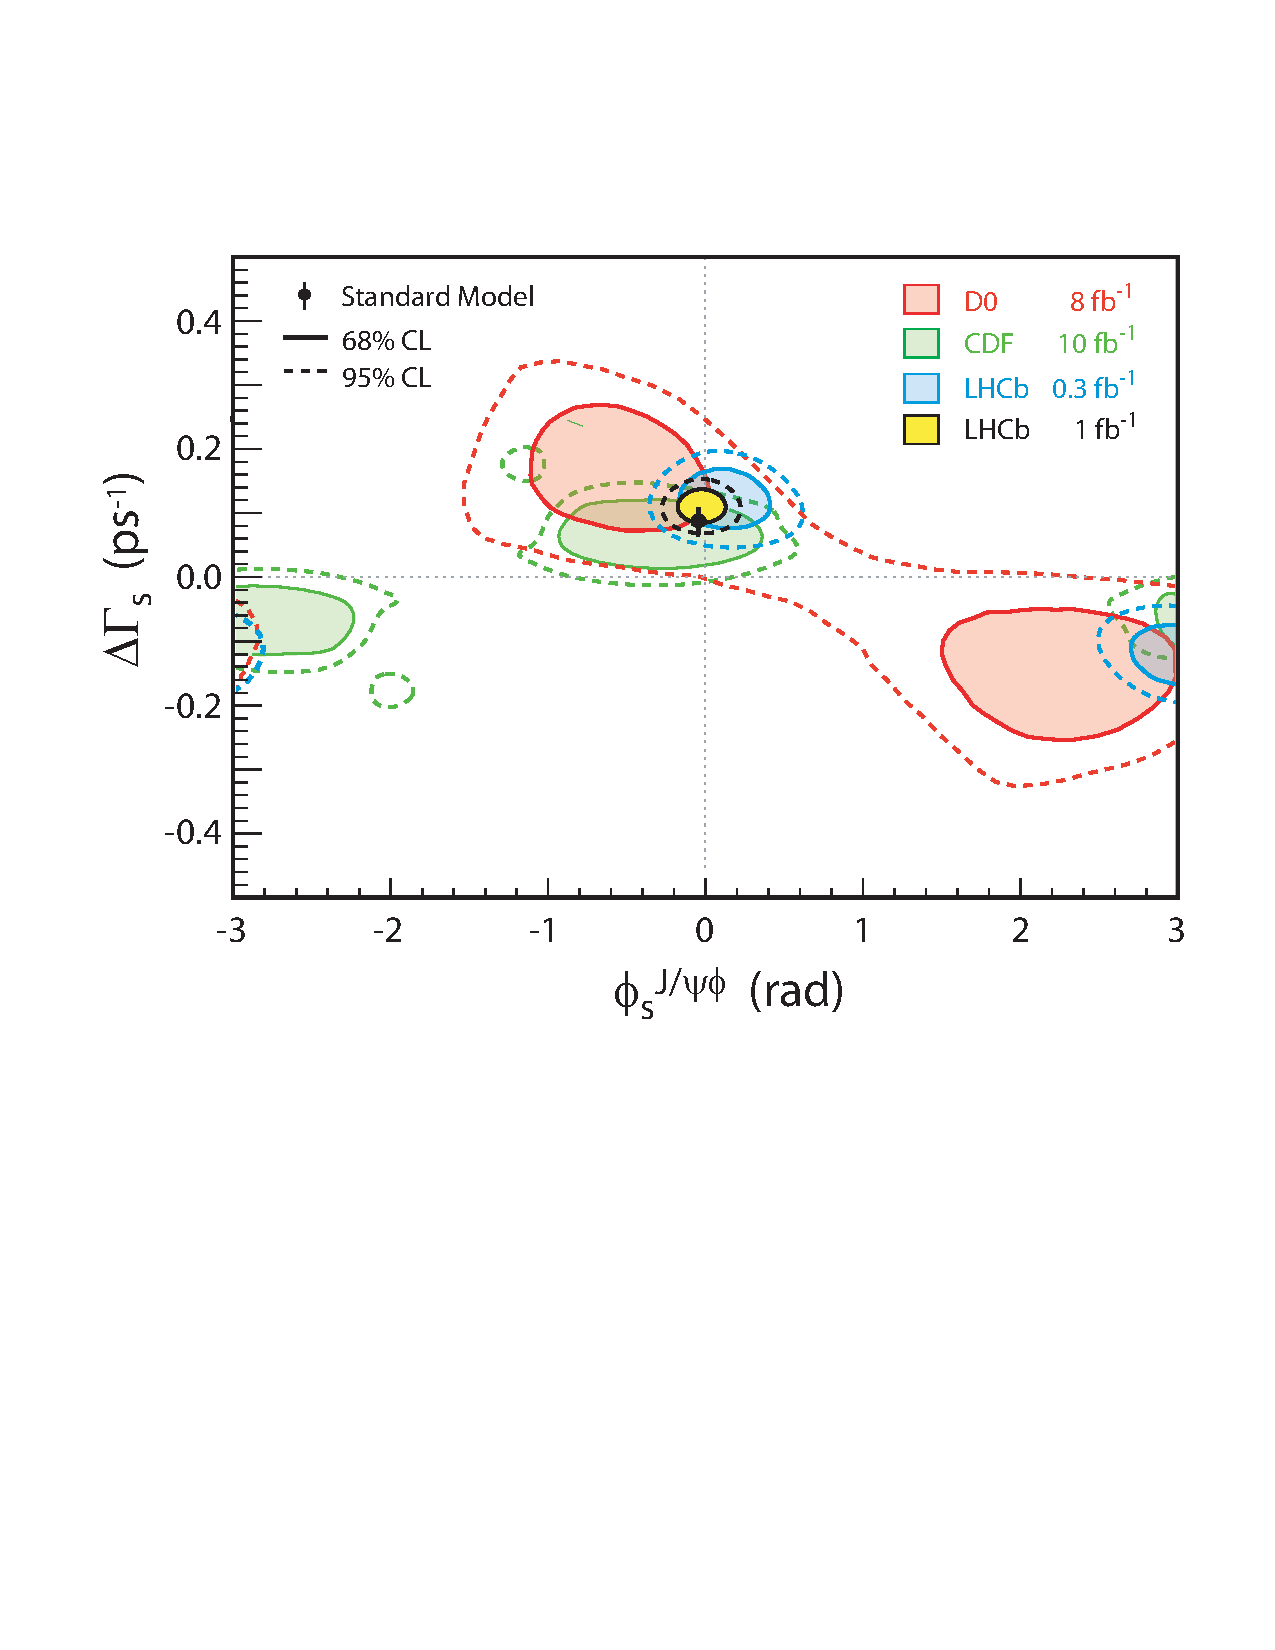
\includegraphics[scale=0.65,bb=50 300 580 700,clip=true]{Roger-plot}
    \vspace*{-1.0cm}
  \end{center}
  \caption{
    \small %captions should be a little bit smaller than main text
    Comparison of our result to those from other experiments.
    Note that the style of this figure differs slightly from that of Figure~\ref{fig:example}}
  \label{fig:roger}
\end{figure}

\clearpage

}

\end{document} 

%
% ****** End of file apssamp.tex ******
